\chapter[The CMS experiment at LHC]{The CMS experiment at LHC}

The CMS experiment is one of the biggest particle physics experiments in the world. It is located on the ring of the LHC that is the main accelerator managed by CERN, the European Organization for Nuclear Research or Centre Europ\'{e}en pour la Recherche Nucl\'{e}aire by its french name. This center constitutes the biggest center for research on particle physics all over the world. All along its 60 years of existence, from 1954, 21 member states have been joining it, but an overall of 113 countries participate in different ways to this center. 

In the present chapter different aspects of the LHC accelerator and the CMS experiment are discussed in detail. In particular some emphasis is made in the CMS sub-detectors related to jets, the objects that play the main role in the search that is the main subject of the present work. The present state of both CMS and LHC experiments, their achievements and the challenges that were overcome are also discussed. Finally, also the expectations and goals for the upcoming run 2 are mentioned.  

\section{The Large Hadron Collider}
\label{sec:LHC}

The Large Hadron Collider, or LHC~\cite{Bruning:782076}, is a machine that accelerates and collides protons and lead ions. This machine is the biggest particle collider nowadays with a circumference of 27 km. It also achieves the highest energy by a collider up to present, planned to be 14~TeV at the center of mass of the collision. On the first run of the machine only 8~TeV were achieved, and next run started with 13~TeV. It is located in French-Swiss border near to Geneva. The tunnel for the machine was carved around 100 m under the ground, 45 m under the Jura mountains and 170 m near the L\'{e}man lake with an inclination of around 1.4\%, sloping down towards the lake. This machine has used as much as possible old LEP buildings and sites, that was an electron-positron collider built between 1984 and 1989. 

The protons and heavy ions accelerated by the machine collide in different points where dedicated experiments are located to detect and study the product from the collisions. The four main experiments located on the LHC ring are ALICE~\cite{Cortese:879894}, ATLAS~\cite{ATLAS:1999}, CMS~\cite{Bayatian:922757,Bayatian:942733} and LHCb~\cite{Alves:2008zz}. ALICE focuses on the study of the quark-gluon plasma produced in heavy ions collisions. ATLAS and CMS are experiments of generic purpose where searches for new physics and also precision measurements are performed. LHCb is dedicated to the physics of the b-quark. Even if one of the principal objectives of the construction of the LHC was the search for the Higgs boson, generic searches on new physics have been conducted from the very beginning of the first data taking in 2009. %Moreover, after the Higgs discovery in 2012 there is a growing effort on the searches for new physics and precision measurement of the properties of the Higgs.

The LHC is a complex machine composed of several parts. The two principal parts are the injector chain and the main ring. A diagram of the whole CERN accelerator complex is shown in figure~\ref{fig:Complex}. The injector chain has different stages that pre-accelerate protons and heavy ions to be injected into the main ring of LHC. %In the main ring the protons and heavy ions are fully accelerated and collided in four different points over the ring.

\begin{figure}[!Hhtbp]
  \begin{center}
    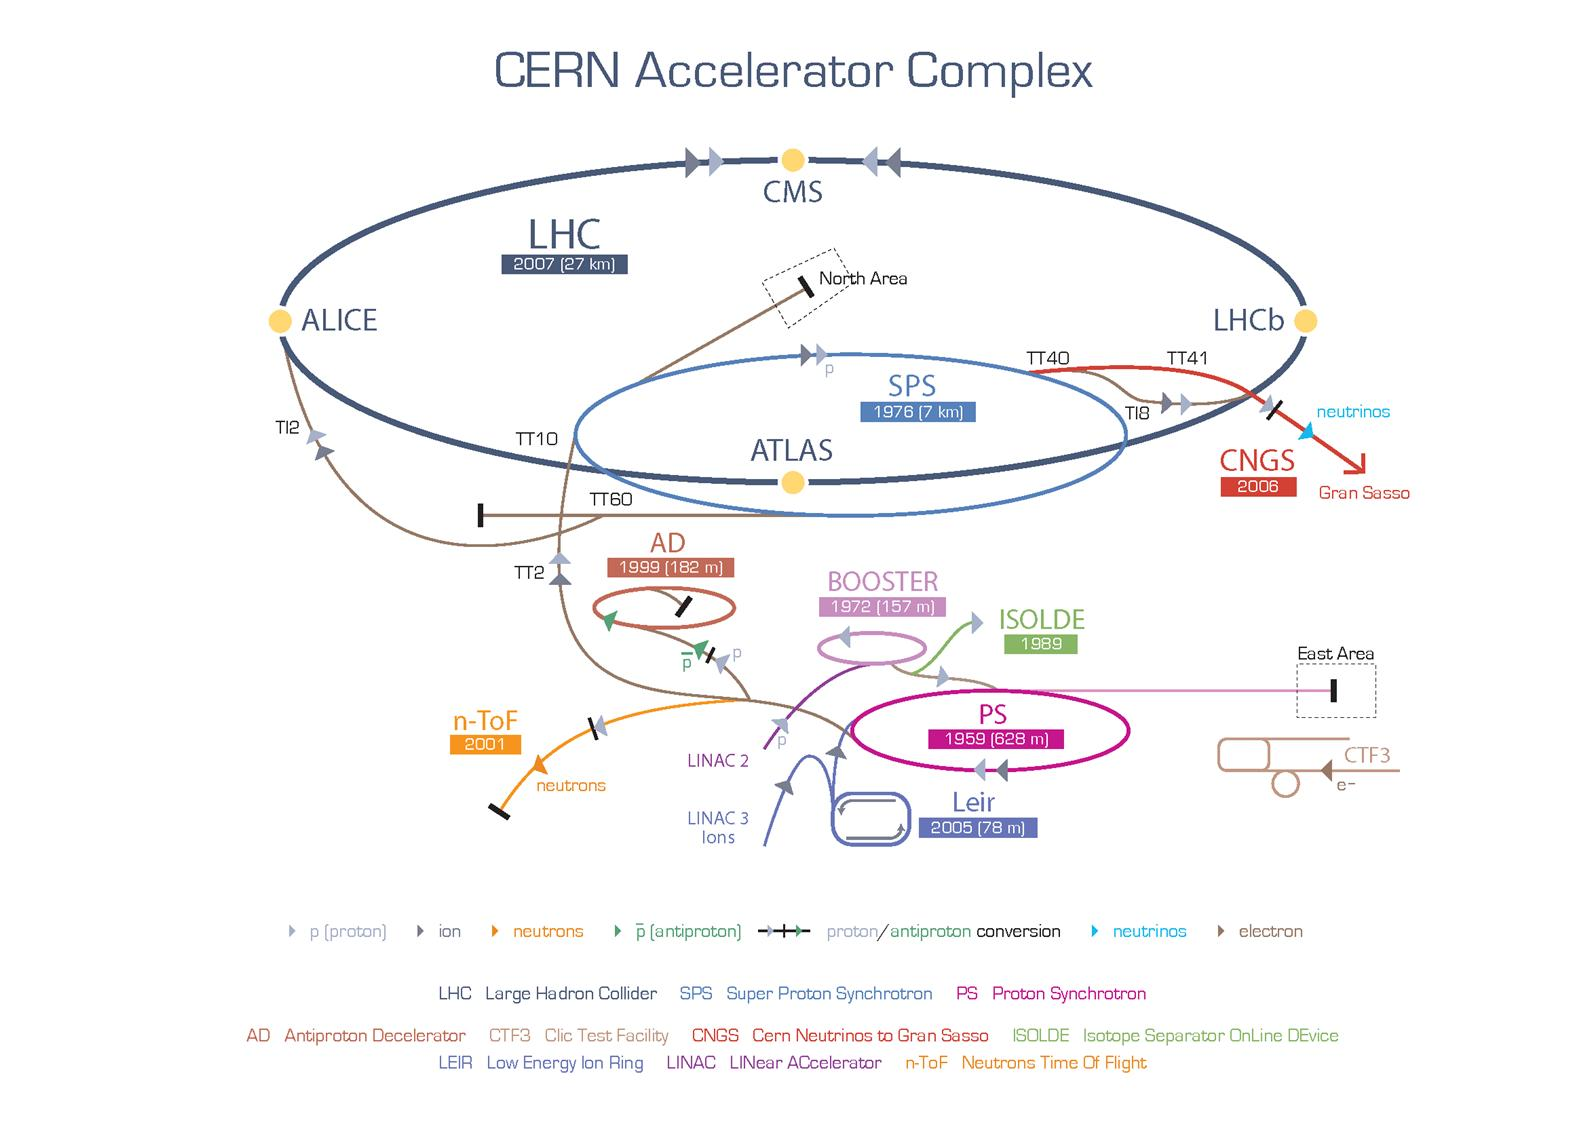
\includegraphics[trim=4.5cm 0cm 0cm 0cm, clip=true, width=1.15\textwidth]{figs/cern-lhc-4.jpg}
    \caption{Organization of CERN accelerator complex}
    \label{fig:Complex}
  \end{center}
\end{figure}

\subsection{Injector chain}
\label{sec:injector}

The injector chain begins with the proton source. Protons are extracted via ionization of Hydrogen gas in the Duoplasmatron Proton Ion Source. Such extraction is pulsed, what makes up the first bunch structure. The extracted protons are then accelerated up to 50 MeV in the linear accelerator, Linac2, that dates from 1978. After this first stage several steps are followed:
\begin{enumerate}
\item Linac2 injects proton bunches in the Proton Synchrotron Booster (PSB) where they are accelerated to 1.4 GeV. 
\item From PSB, the protons are delivered to the Proton Synchrotron (PS) where they reach an energy of 28 GeV. In the PS the bunches are also split from 6 initial bunches to 72 spaced by 25 ns.
\item Finally, the pre-acceleration chain is finished by the SPS, Super Proton Synchrotron. There the bunches are accelerated up to 450 GeV right before being inserted into the main LHC ring. 
\end{enumerate}

The whole pre-acceleration chain has been optimized to obtain the best possible performance on the final acceleration in the LHC main ring. All parameters are carefully controlled, for example the number of bunches, the separation between bunches, the separation between trains of bunches or the injection energy to each subsystem. It's also remarkable to notice the level of control achieved in the bunches manipulation, from old subsystems as the PS from 1959 or the newest, the SPS that dates from 1976. 

%Some recent plans for future accelerator have been studied using the LHC main ring as injector for a bigger accelerator, for example the so called FCC (Future Circular Collider) at CERN. The FCC could be built to perform proton-proton, electron-positron or electron-proton collisions, versions that are called respectively FCC-hh, FCC-ee and FCC-he. The FCC-hh is being designed to achieve 100 TeV of center of mass energy in a tunnel of 80-100 km of circumference. 

\subsection{LHC main ring}
\label{sec:ring}

The main ring is composed of two rings that accelerate the proton bunches in opposite directions, clock-wise and counter clock-wise. An schematic view of the design of the main ring can be seen in figure~\ref{fig:schematic}. The rings crosses in different points in order to collide the protons and they are divided in eight straight sections and eight arcs. In each octant bunches are controlled by dipole magnets. These complex magnets, in figure~\ref{fig:dipole}, need to produce a very strong magnetic field in order to be able to bend a 7~TeV beam of protons. This intense magnetic field, 8.33~T, in opposite directions, is produced by electrical currents that are only achievable by means of superconductivity. All the 1232 dipoles operate at a temperature of 1.9~K, under cooling by liquid helium. They also operate under ultra-high-vacuum. The beam lines with a pressure less than $10^{-9}$ mbar and the whole dipole system with $10^{-6}$ mbar, that serves also as insulating system from the surroundings. In addition, the LHC main ring has other magnets that focus and correct different characteristics of the beam: 520 quadrupoles, 2464 sextupoles, 1232 octupoles. 

\begin{figure}[!Hhtbp]
  \begin{center}
    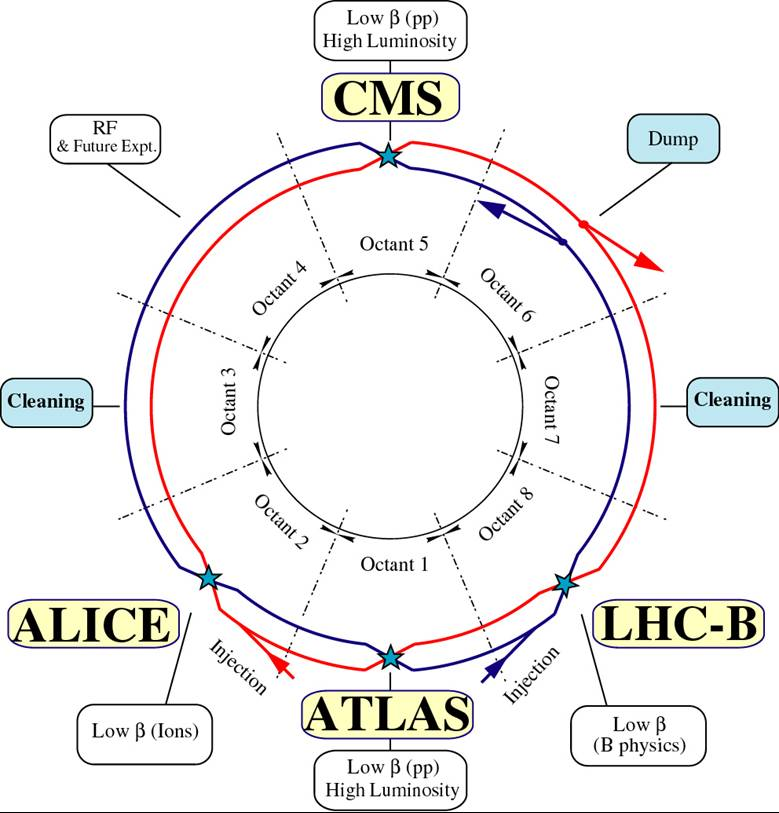
\includegraphics[width=0.8\textwidth]{figs/lhc-schematic.jpg}
    \caption{Schematic of the LHC main ring design.}
    \label{fig:schematic}
  \end{center}
\end{figure}

\begin{figure}[!Hhtbp]
  \begin{center}
    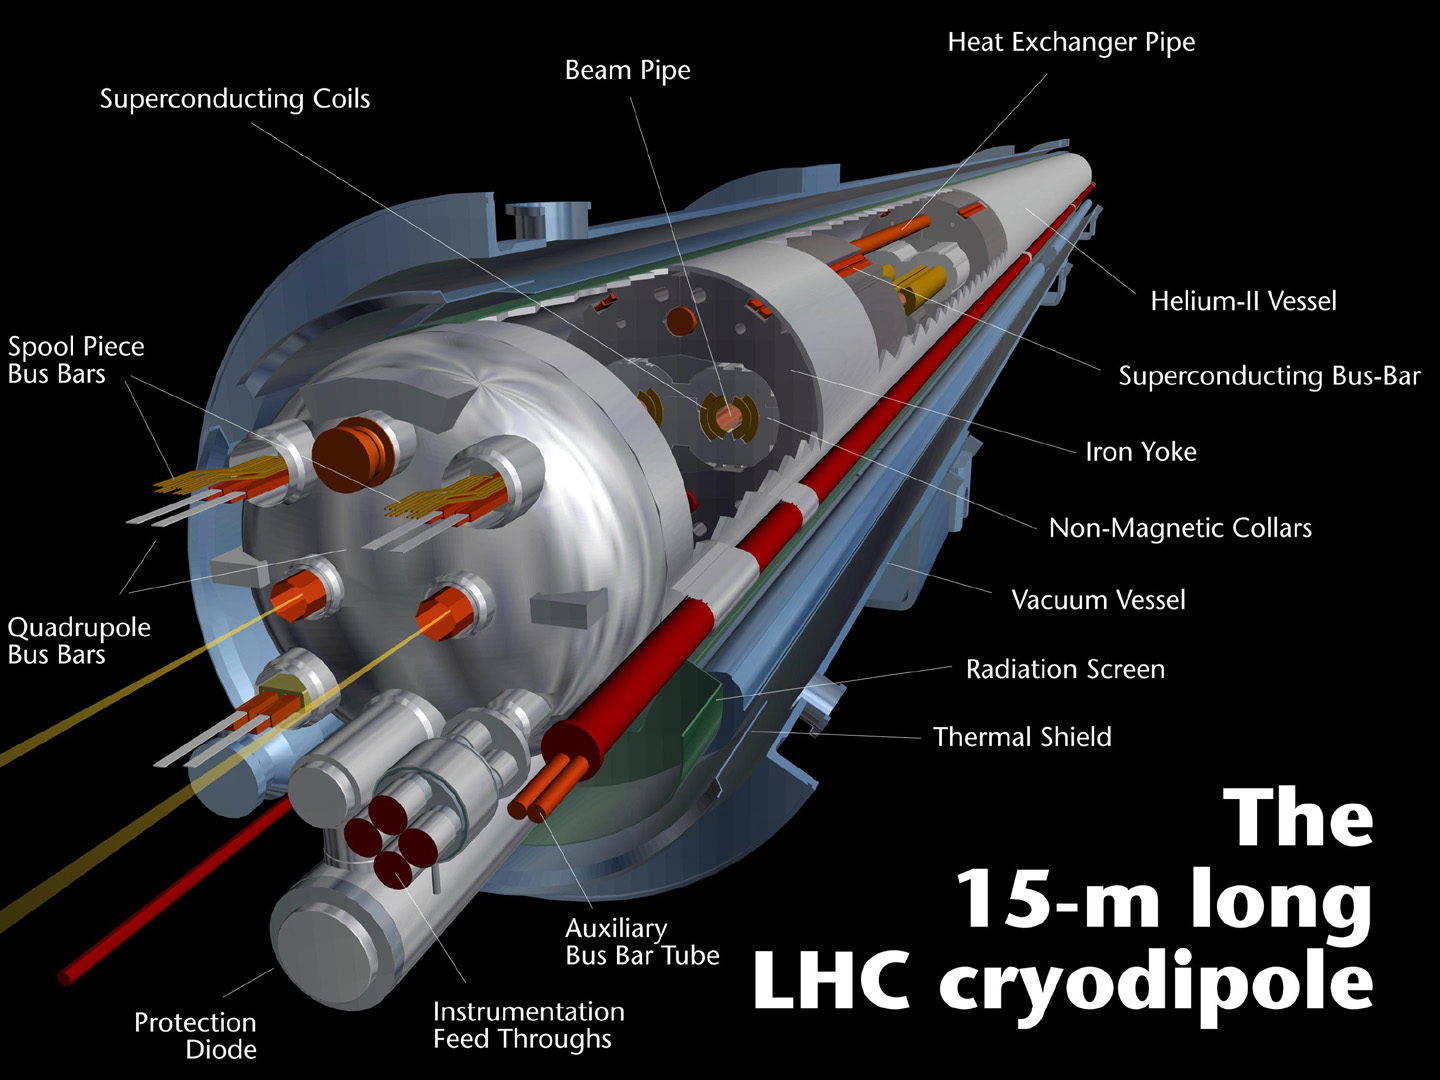
\includegraphics[width=0.45\textwidth]{figs/cryodipole.jpg}
    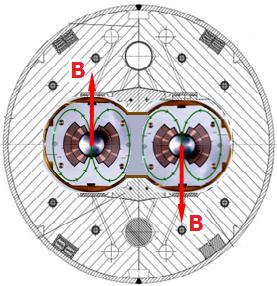
\includegraphics[width=0.45\textwidth]{figs/dipole_B.jpg}
    \caption{Design of LHC cryodipole and the magnetic field that bends the beam in the main ring.}
    \label{fig:dipole}
  \end{center}
\end{figure}

\subsubsection{Luminosity}
\label{sec:lumi}

In collider physics, such as the LHC, the figure of merit is the luminosity, given in equation~\ref{eq:lumiC}. 

\begin{equation}
  \label{eq:lumiC}
  L=\frac{k_{b}N_{b}^{2}f_{rev}\gamma}{4\pi\epsilon_{n}\beta^{*}}R=\frac{k_{b}N_{b}^{2}f_{rev}}{4\pi\sigma^{*}_{x}\sigma^{*}_{y}}R
\end{equation}

The number of events per second is proportional to the luminosity, hence is the quantity to be maximized by the design and operation of the accelerator. The collider characteristics depend on the number of bunches in the ring $k_{b}$, the number of protons per bunch $N_{b}$, the revolution frequency $f_{rev}$, the relativistic gamma factor $\gamma$, the normalized rms transverse beam emittance $\epsilon_{n}$ and the beta function at the interaction point $\beta^{*}$. The denominator on~\ref{eq:lumiC} can also be rewritten in terms of the horizontal and vertical width of the bunches at the crossing, $\sigma^{*}_{x}$ and $\sigma^{*}_{y}$. In addition, there is the geometric reduction factor ($R$) that introduces a dependence with the crossing angle of the bunches at the interaction points, with a value around 0.8 for nominal LHC conditions. The crossing angle refers to the angle at which the bunches are crossed in the collision points of LHC. In table~\ref{tab:LHCparams} the LHC beam parameters at injection and collision are presented.  

\begin{table}[htbH]
%\label{tab:LHCparams}
\begin{center}
\caption{LHC proton beam designed parameters.\label{tab:LHCparams}}
%\resizebox{\textwidth}{!}{
\begin{tabular}{|c|c c|}
\hline 
Parameter/units & Injection & Collision \\
\hline
Energy [GeV]& 450 & 7000 \\ 
Luminosity [$\text{cm}^{-2}\text{s}^{-1}$] & & $10^{34}$ \\
$k_{b}$ Number of bunches & \multicolumn{2}{c|}{2808} \\
Bunch spacing [ns] & \multicolumn{2}{c|}{24.95} \\
$N_{b}$ intensity per bunch [protons/bunch] & \multicolumn{2}{c|}{$1.15\times 10^{11}$} \\
Beam current [A] & \multicolumn{2}{c|}{0.58} \\
$\epsilon_{n}$ normalized rms transverse beam emittance [$\mu$m] & 3.5 & 3.75 \\ 
$f_{rev}$ revolution frequency [kHz] & \multicolumn{2}{c|}{11.25} \\
\hline
\end{tabular}
%}
\end{center}
\end{table}

At the crossing points, the number of events coming from collisions and produced via a specific process, is directly proportional to the luminosity provided by the collider, as in equation~\ref{eq:lumiC}.

\begin{equation}
  \label{eq:lumiN}
  N_{events}=L\sigma_{process}
\end{equation} where $\sigma_{process}$ is the cross section of the process. 

The total cross section of a proton-proton collision from the crossing of two bunches at 14 TeV is 100-110 mb~\cite{Augier:1993ta}, from three different scattering processes: elastic, diffractive and inelastic. In the elastic scattering the protons only exchange momenta but their structure remain unchanged, that is the case for the majority of collisions. In diffractive scattering processes not only momenta is exchanged but also new particles are produced in addition to the two final protons. Finally, in inelastic scattering, the constituents of the protons, the partons, interchange a big amount of momentum and produce a large quantity of particles. The inelastic processes contribute less than diffraction to the total cross section. While inelastic collisions produce particles in the central rapidity (defined in~\ref{sec:Csys}) region, diffractive and elastic final products have a large rapidity. Only in the hard interactions, inelastic scattering, color is exchanged, being the reason to fill up the central rapidity region. 

From the crossing of two bunches not only one proton-proton interaction is expected. The number of expected interactions in each crossing depends on the run settings. From LHC design, a mean number of $<20>$ pileup interactions are expected at 25 ns for 14 TeV. From them, only one is coming from an inelastic collision with a high exchange of momentum, that is the type of process of more interest for detectors as ATLAS or CMS. This fact puts an additional difficulty to the detectors in order to extract the hard interaction from all the elastic and diffractive collisions happening at same time. Such phenomena is known as Pile-Up, an illustration of a collision with high pile-up can be found on figure~\ref{fig:pileup} as seen by the CMS detector.

\begin{figure}[!Hhtbp]
  \begin{center}
    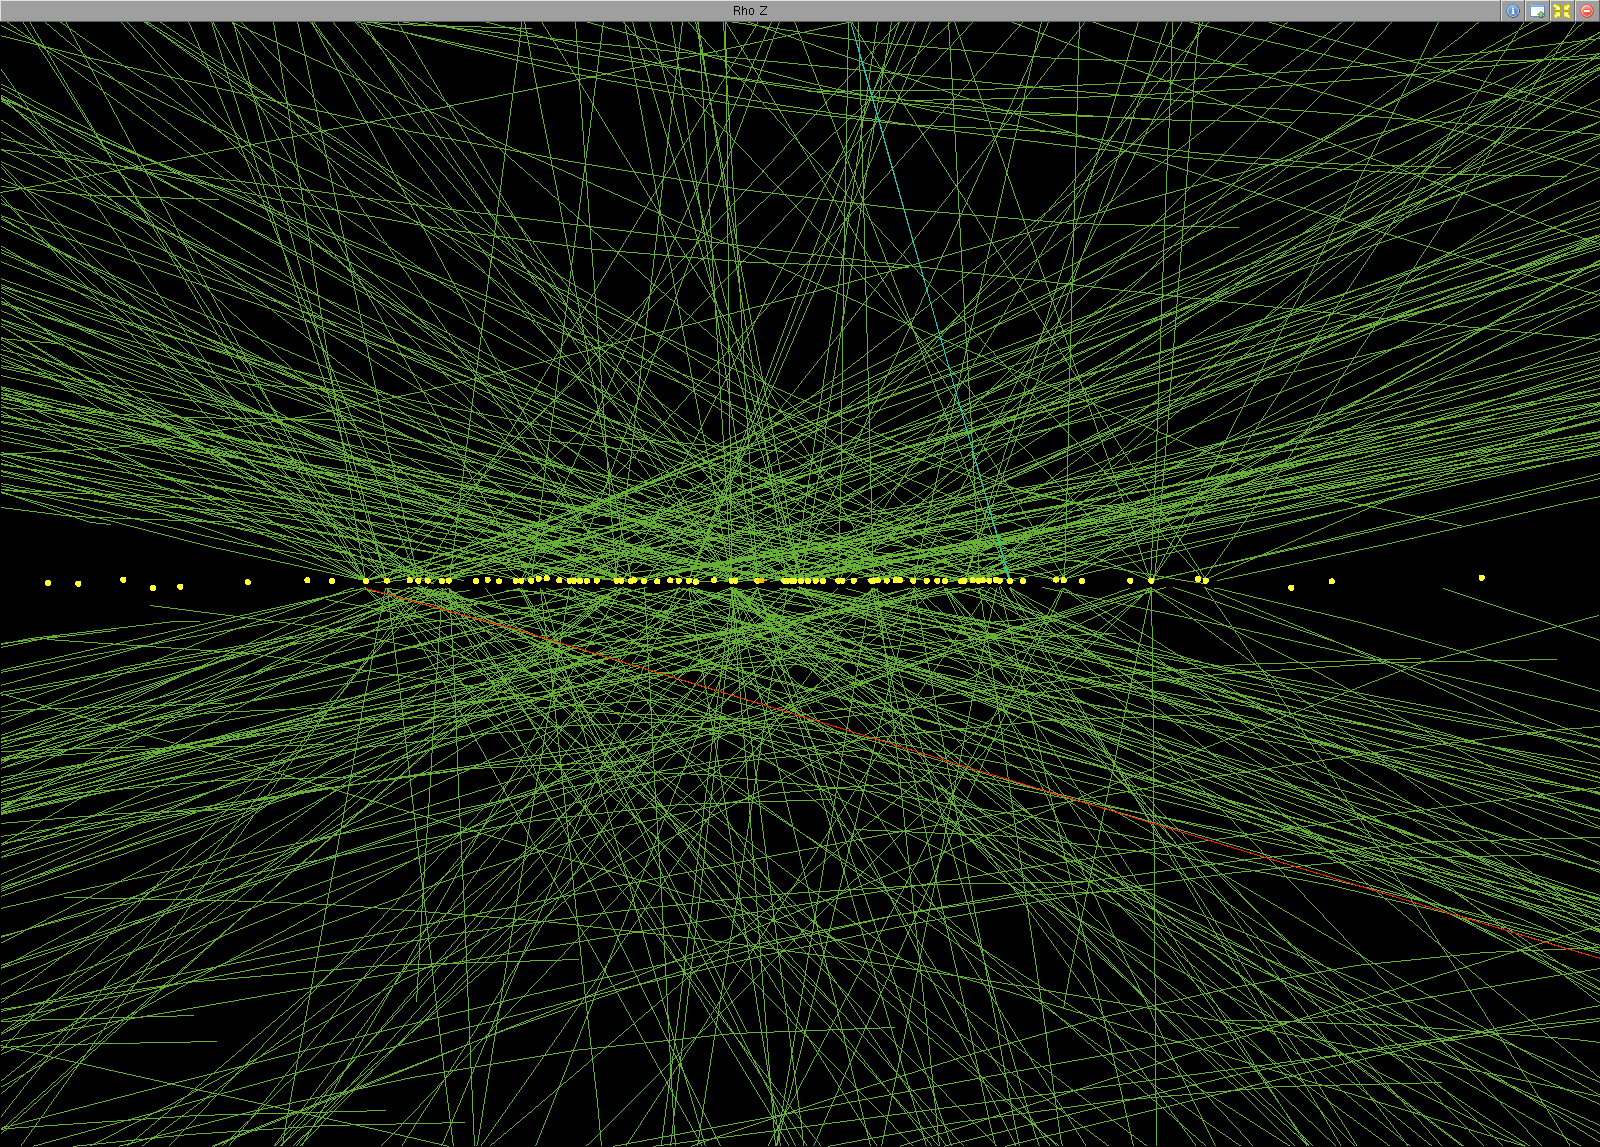
\includegraphics[width=0.7\textwidth]{figs/pileup.png}
    \caption{High pile-up event (78 interactions) seen by CMS detector. Event 35655522, from 198609 run, lumi 56, recorded on 2012.}% Image credit: Andre Holzner }
    \label{fig:pileup}
  \end{center}
\end{figure}

\subsection{Run 1}
\label{sec:run1}

On February 10 of 2013 the first stable run of the LHC reached an end. This run, now called Run 1, started on November 20 of 2009. LHC was originally planned to start in 2008, but an incident on one of the electric connections of one of the magnets forced to stop on the 19th of September of the same year. From the restart in 2009, the energy was augmented from 450 GeV to 4 TeV per beam. The 23th of September 2009 the first collisions were detected by the experiments. One week after, the achieved center of mass energy was $\sqrt{s}=2.36$ TeV, already higher than Tevatron (1.96 TeV).

In 2010, from 30th March to 6th December 3.5 TeV per beam were reached delivering near 50 $\text{pb}^{-1}$. With the same energy, approximately 6 $\text{fb}^{-1}$ were delivered in 2011. 

In 2012, the center of mass energy reached one additional TeV, $\sqrt{s}=8$ TeV, and around 20 $\text{fb}^{-1}$ of integrated luminosity were delivered between April and December. The data produced in this period is going to be used in the analysis presented in chapter~\ref{chap:search}. Figure~\ref{fig:CMSlumi} shows the progress of the recorded luminosity by CMS for 2010-2012 period. The first six weeks of 2013 were devoted to proton-lead collisions.

After this very successful run, the LHC has been stopped for about 2 years for repair and maintenance of different systems in the experiments and in the LHC itself to achieve higher energies. After this period, known as Long Shutdown  or LS1, the LHC restarted a new run in spring 2015.

\begin{figure}[!Hhtbp]
  \begin{center}
    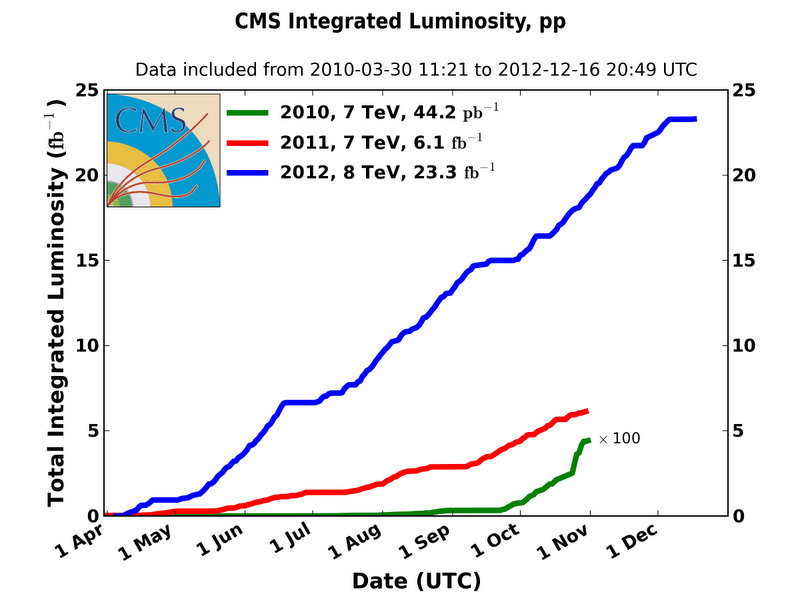
\includegraphics[width=0.7\textwidth]{figs/cms-int-10to12.jpg}
    \caption{CMS integrated luminosity for proton-proton collisions delivered by LHC. }
    \label{fig:CMSlumi}
  \end{center}
\end{figure}

\subsection{Other experiments at LHC}
\label{sec:expers}

LHC main ring delivers collisions to various experiments. The biggest are ATLAS~\cite{ATLAS:1999} and CMS~\cite{Bayatian:922757}, both of them generalist experiments designed to do precision measurements as well as new physics searches. Mainly recording proton-proton collisions, they have also recorded lead-lead and proton-lead collisions during the run 1. Both of them were designed for high instantaneous luminosity, $L = 10^{34}\text{cm}^{2}\text{s}^{-1}$.

In addition, there are two other experiments designed for specific purposes. ALICE~\cite{Cortese:879894} built for the study of strongly interacting matter and LHCb~\cite{Alves:2008zz} that focus on the study of the physics of the b-hadrons, specially related to the CP violation. The first of them record proton-proton collisions at an instantaneous luminosity of $10^{32}\text{cm}^{2}\text{s}^{-1}$ and the second record ion-ion collision with $L = 10^{27}\text{cm}^{2}\text{s}^{-1}$.

The CMS experiment is going to be described in detail in section~\ref{sec:CMS}. In the following sections we are going to present very briefly the other three experiments mentioned above. 

\subsubsection{ALICE}
\label{sec:alice}

The ALICE experiment (A Large Ion Collider Experiment) is located at point 2 of the LHC main ring, measures 16 m high, 16 m wide and 26 m long, and weights 10000 tons. Designed for heavy ion physics, it is able to detect an extremely high number of tracks per event. Its main subsystem is the Time Projection Chamber (TPC), a 90 $\text{m}^{3}$ gas chamber filled with a mixture of Ne, $\text{CO}_{2}$ and $\text{N}_{2}$ operated in a solenoid of 0.5 T. It allows to measure leptonic and hadronic charged particles in a momentum range from 0.5 to 10 GeV/c. The experiment structure can be seen on figure~\ref{fig:alicedet}. ALICE collaboration counts around 1500 people, from 154 physics institutes in 37 countries.

\begin{figure}[!Hhtbp]
  \begin{center}
    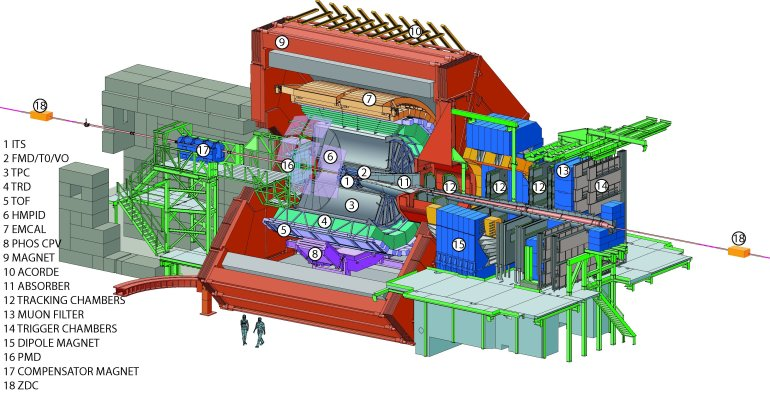
\includegraphics[width=0.8\textwidth]{figs/alice2.jpg}
    \caption{ALICE detector.}
    \label{fig:alicedet}
  \end{center}
\end{figure}

\subsubsection{ATLAS}
\label{sec:atlas}

The ATLAS experiment (A Toroidal LHC ApparatuS) is the biggest LHC experiment. It's located at point one, as displayed on figure~\ref{fig:schematic}, on the LHC main ring. It's a cylindrical detector similar to CMS, about 45 meter long, 25 meter high, and weights around 7000 tons. ATLAS main components are, from inside to outside, a tracking system, an electromagnetic calorimeter, a hadron calorimeter and muon chambers. In between these subsystems there is an internal solenoidal magnet and a set of external toroidal magnets. Its main technology for calorimetry is liquid Argon. The detector design is presented on figure~\ref{fig:atlasdet}.

\begin{figure}[!Hhtbp]
  \begin{center}
    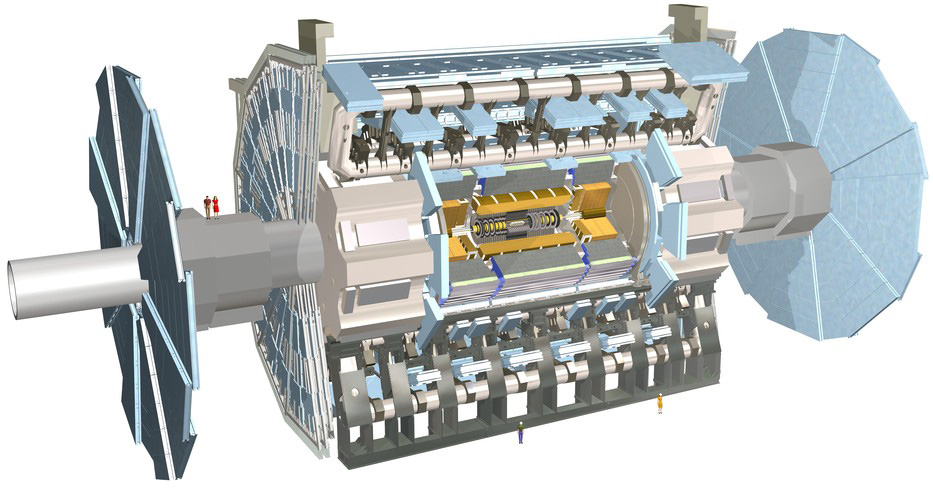
\includegraphics[width=0.7\textwidth]{figs/atlas_lg.jpg}
    \caption{ATLAS detector internal view. }
    \label{fig:atlasdet}
  \end{center}
\end{figure}

ATLAS experiment configures a collaboration of around 3000 persons, coming from 117 universities around the world, from 38 countries.

\subsubsection{LHCb}
\label{sec:lhcb}

LHCb detector, hosted at point 8 of the LHC main ring, has a different design than ATLAS and CMS. Smaller than these, it has been designed to be able to detect particles produced close to the beam direction. This is the reason why it is not cylindrically but conically shaped, in two detection arms, as shown in figure~\ref{fig:lhcbdet}. It also has the same main parts, a tracking system, electromagnetic and hadron calorimeters, muon chambers and magnets. Its major specificity is a system that allows to identify different hadrons, the RICH detectors, a crucial feature for the study of strong interacting matter. In addition, the tracker system counts with a very precise vertex locator system. It measures 21 m long, 10 m high and 13 m wide, and weights 4500 tons. The LHCb collaboration groups around 700 persons from 69 different universities over 17 countries. 

\begin{figure}[!Hhtbp]
  \begin{center}
    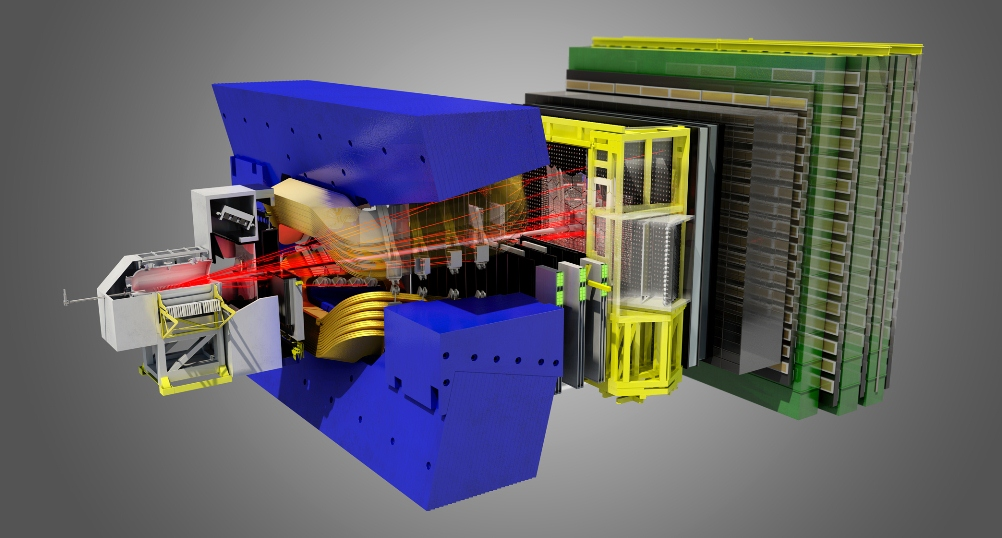
\includegraphics[width=0.8\textwidth]{figs/LHCbDetectorlight1.jpg}
    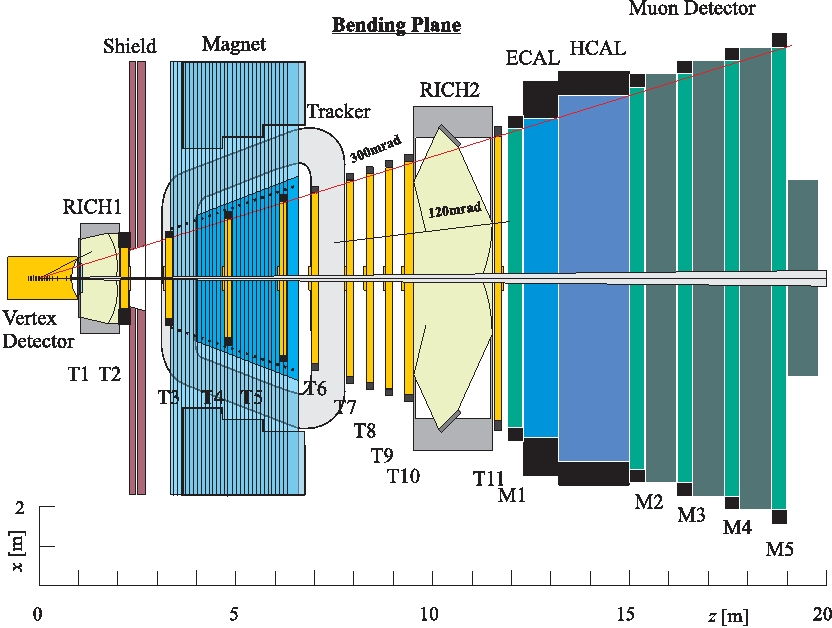
\includegraphics[width=0.8\textwidth]{figs/LHCb_UpView.jpg}
    \caption{LHCb detector 3D view [top] and view from the top [bottom]. }
    \label{fig:lhcbdet}
  \end{center}
\end{figure}

%\begin{figure}[!Hhtbp]
%  \begin{center}
%    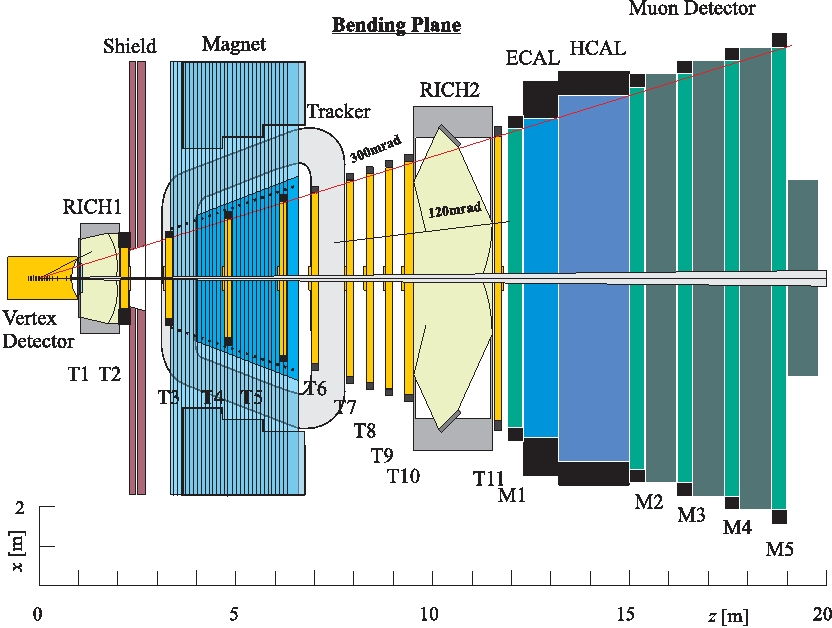
\includegraphics[width=0.7\textwidth]{figs/LHCb_UpView.jpg}
%    \caption{LHCb detector view from the top. }
%    \label{fig:lhcbupview}
%  \end{center}
%\end{figure}

\section{The Compact Muon Solenoid (CMS) experiment}
\label{sec:CMS}

The CMS detector, hosted at point 5 of the LHC main ring (see figure~\ref{fig:schematic}), is the second biggest LHC experiment. Cylindrically shaped, it measures 15 m of diameter and 28.7 m long, and it weights 14000 tons, making it the heaviest LHC experiment. Its subsystems are concentrically located from the beam line. It's called compact because the whole calorimetry is inside the solenoid magnet, and muon solenoid because it has a very precise muon detection. Its main characteristic is the strong 3.8 T superconductor solenoid magnet. A representation of the detector can be found in figure~\ref{fig:cmsdet}. The CMS collaboration is formed by around 3500 scientists from 181 institutes over 41 countries. 

\begin{figure}[!Hhtbp]
  \begin{center}
    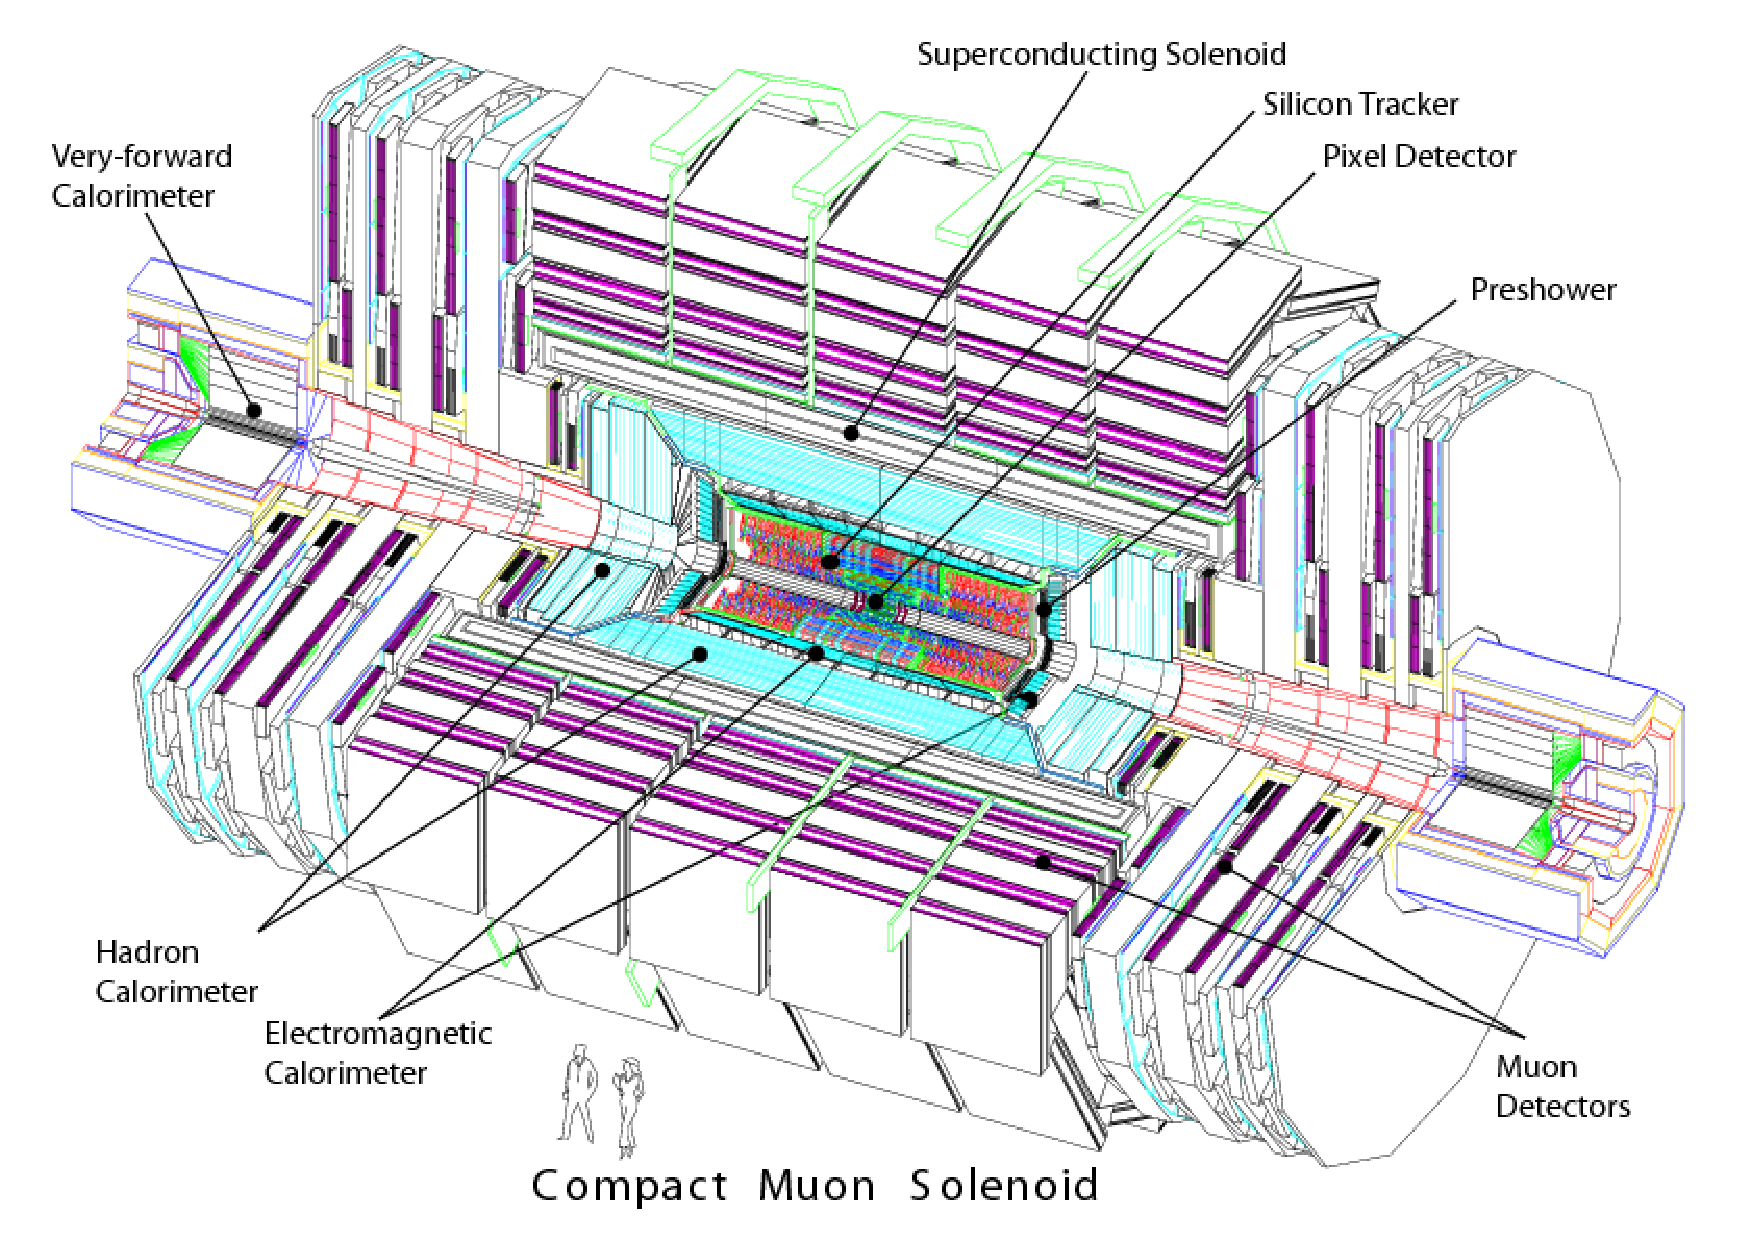
\includegraphics[width=\textwidth]{figs/CMS_det.pdf}
    \caption{CMS detector.}
    \label{fig:cmsdet}
  \end{center}
\end{figure}

CMS has been designed to be able to do very precise identification of particles and their properties. For example, the energy of jets can be determined with an uncertainty smaller than 4\% for jet with a \ptg{20}. Details on other objects will be given later in this section. For the measurement of the momentum of the charged particles, CMS counts with a very powerful magnet that allows to bend very energetic particles. In addition, the calorimeters allow to measure accurately the energy from hadrons, electrons and photons. At the most external layer, the muons chambers measuring muons properties, and in the innermost the tracking system that reconstructs the collision points and the charged particles tracks. In figure~\ref{fig:cmsslice} a representation of the different subsystems of CMS and how particles are reconstructed from them is displayed.

\begin{figure}[!Hhtbp]
  \begin{center}
    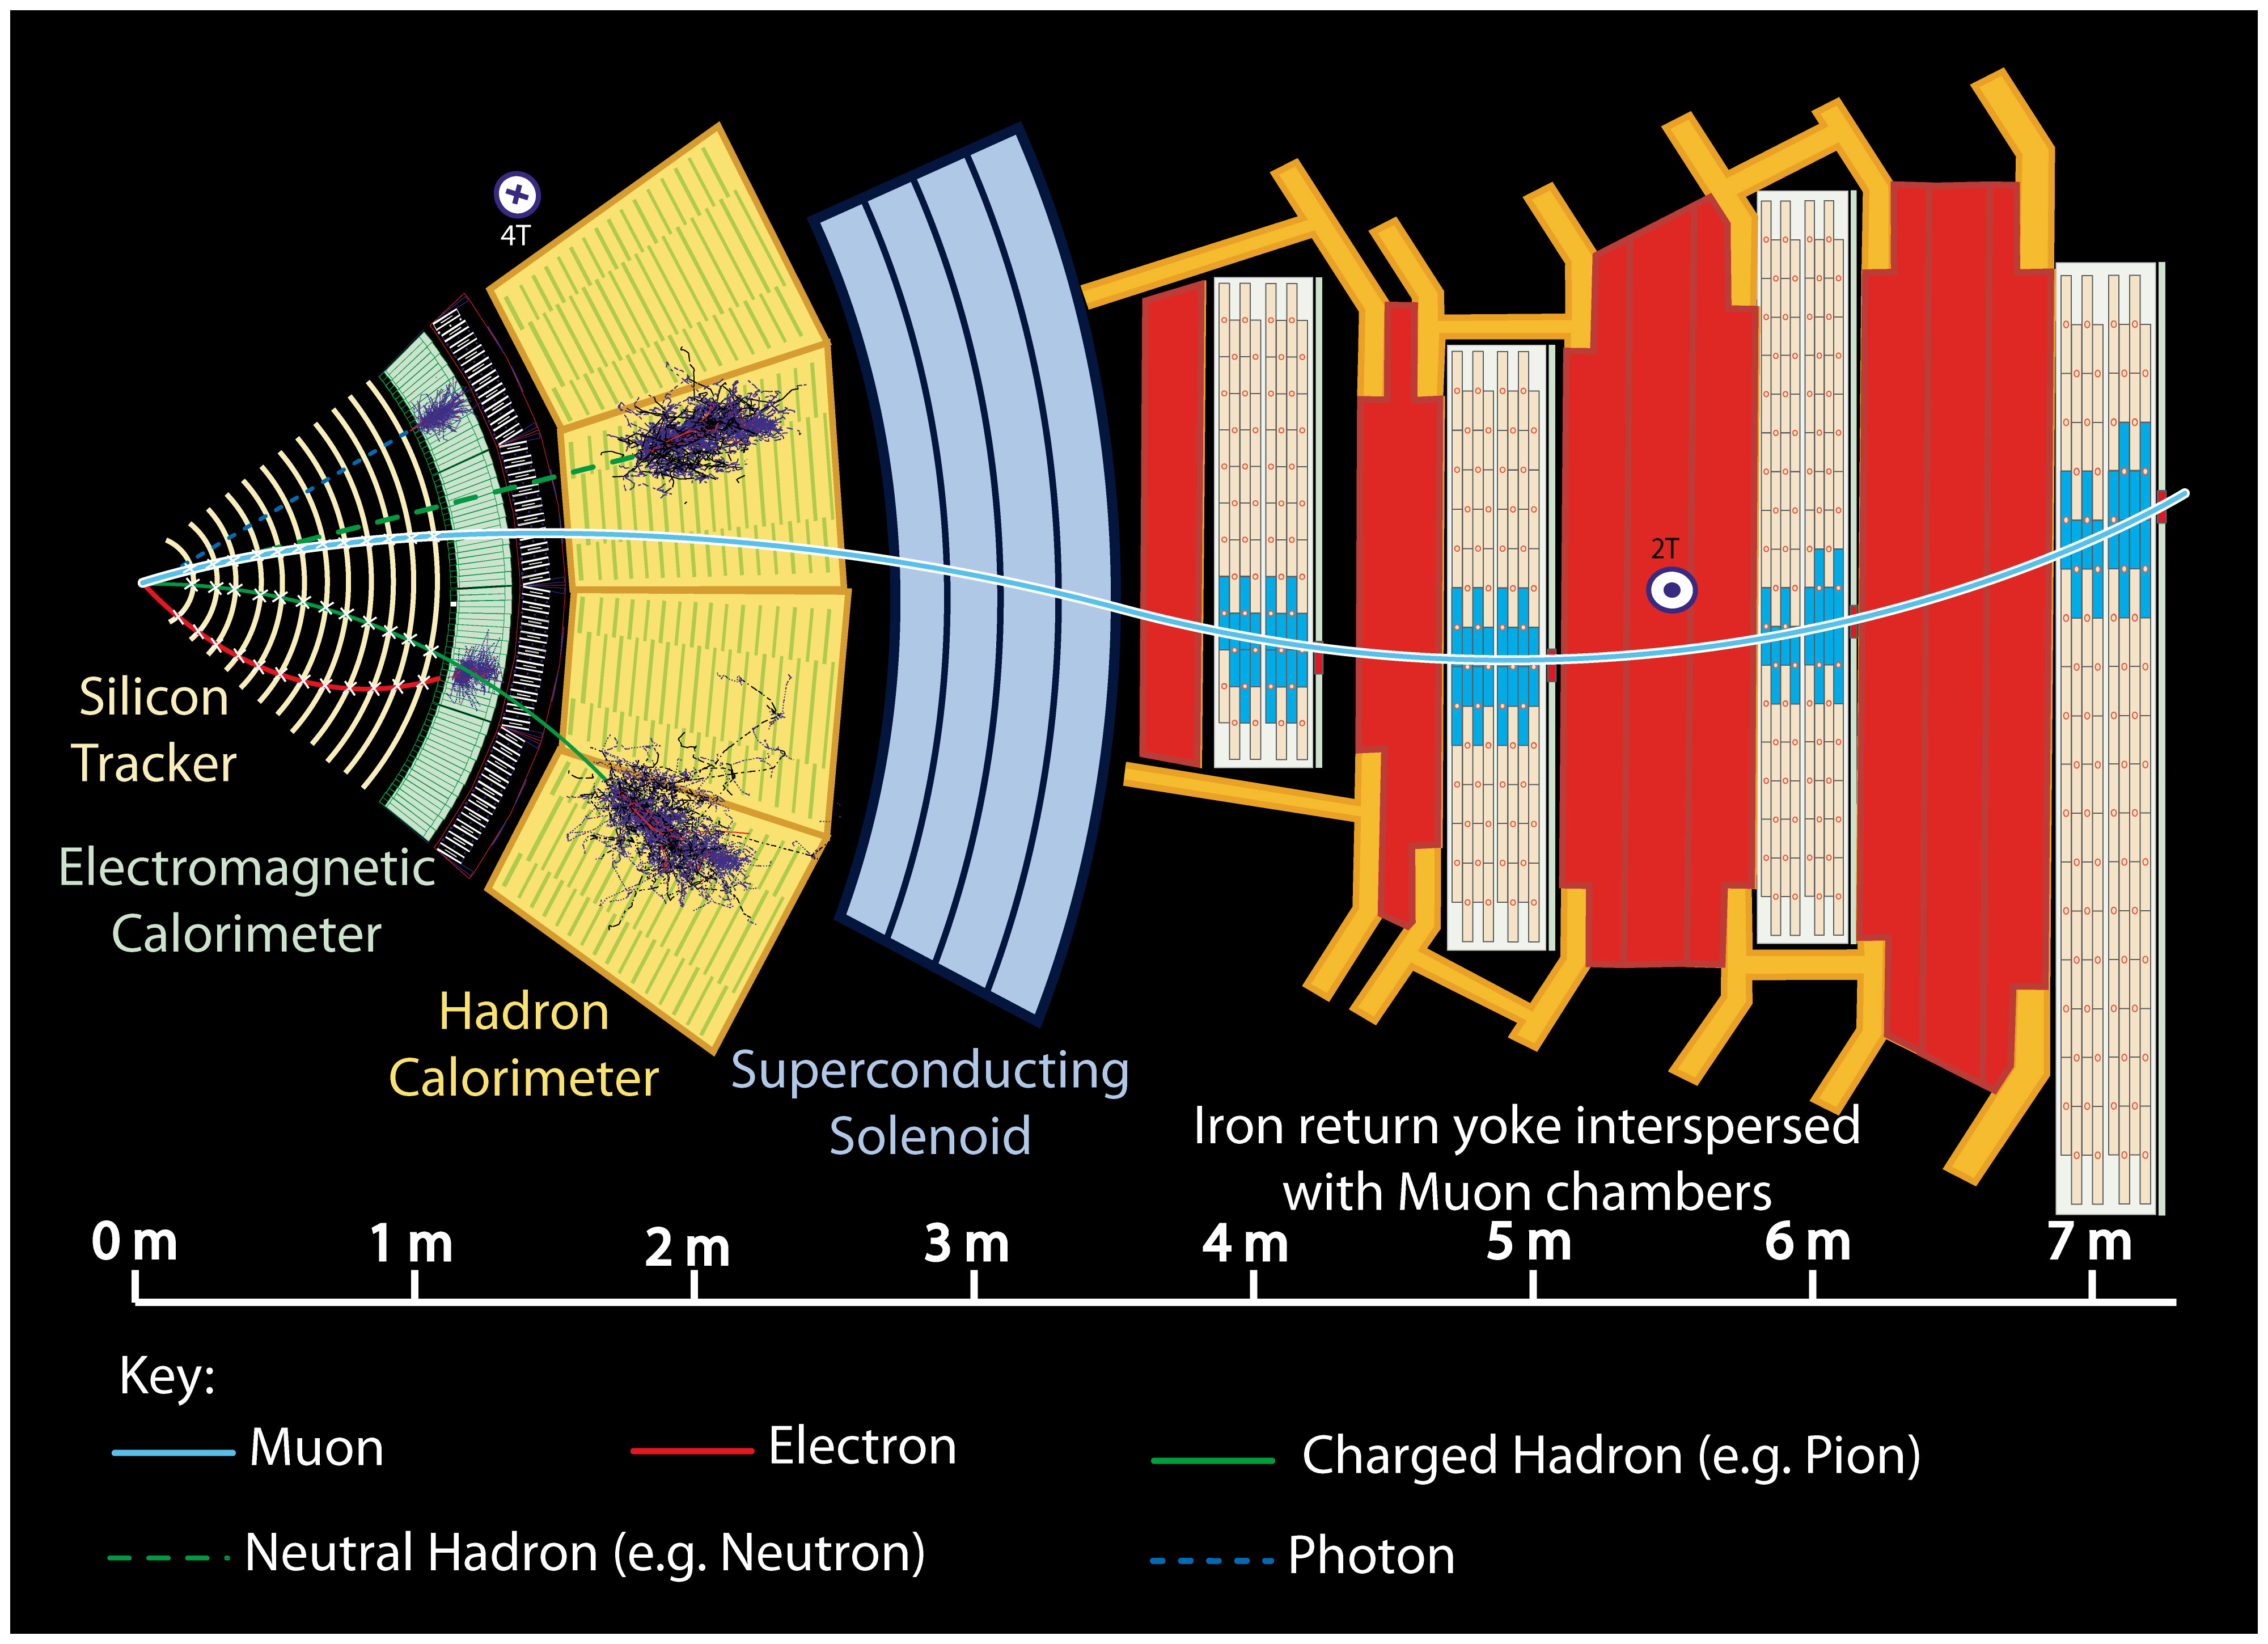
\includegraphics[width=\textwidth]{figs/PictureforPoint5_oct04_allp.jpg}
    \caption{CMS sub-detectors and particle identification. }
    \label{fig:cmsslice}
  \end{center}
\end{figure}

In the following subsections the different subsystems of the CMS experiment are described. In first place, the definition of the coordinate system followed by the description of CMS magnet are given. As last point, a description of the trigger system is presented. 

\subsection{Coordinate system}
\label{sec:Csys}

The origin of coordinates defined on the CMS detector is located at its center. This center is the nominal collision point, the ``interaction point''. From there, the z-axis is defined along the beam pipe line pointing towards the Jura mountains. The positive/negative z-axis directions define the positive/negative sides of the detector. The y-axis is defined towards the zenith and the x-axis towards the center of the LHC ring. Due to the inclination of the LHC plane, this coordinate system is slightly tilted with respect to the true vertical. A representation of the coordinate system definition can be found in figure~\ref{fig:cmscoor}. 

\begin{figure}[!Hhtbp]
  \begin{center}
    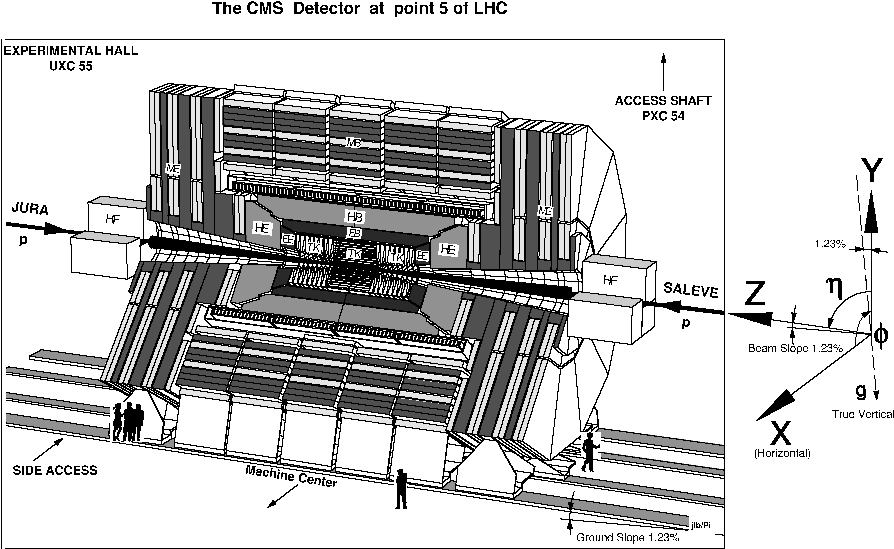
\includegraphics[width=\textwidth]{figs/CMS_coordinates.jpg}
    \caption{CMS coordinate system. }
    \label{fig:cmscoor}
  \end{center}
\end{figure}

Two angles are defined: the $\phi$ angle in the x-y plane from the x-axis towards the positive y-axis, and the $\theta$ angle in the z-y plane from z-axis towards the positive y-axis. In experimental particle physics, it is preferred to work with relativistic invariant quantities, reason why instead of working with $\theta$ we define the pseudorapidity $\eta$, equation~\ref{eq:pseudorapidity}. 

\begin{equation}
  \label{eq:pseudorapidity}
  \eta = -\text{ln}\left( \text{tan}\left(\frac{\theta}{2}\right)\right)
\end{equation} 

Another relativistic invariant quantity can be defined, the rapidity $y$ as from equation~\ref{eq:rapidity}. With $\vec{p}$ being the momentum vector and $E$ the energy of a given particle, $p_{L}$ denotes its longitudinal component, that in our case is the same z-component. 

\begin{equation}
  \label{eq:rapidity}
  y=\frac{1}{2}\text{ln}\left(\frac{E+p_{L}}{E-p_{L}}\right)
\end{equation} On the limit that the mass of the particle is very small compared to its momentum, the particle energy can be approximated by the momentum magnitude, giving rise to the definition of the pseudorapidity in terms of the momentum of the particle $\eta = \frac{1}{2}\text{ln}\left(\frac{\bm{p}+p_{L}}{\bm{p}-p_{L}}\right)$

The radial coordinate is defined over the x-y plane, plane that is called the transverse plane being orthogonal to the longitudinal direction, the z-axis. In such plane are also defined the transverse quantities of particles, as the transverse momentum $p_{T}$. Finally, for any two objects an angular distance can be defined in the $\eta-\phi$ plane, as in equation~\ref{eq:deltaR}.

\begin{equation}
  \label{eq:deltaR}
  \Delta R=\sqrt{(\Delta\eta)^{2}+(\Delta\phi)^{2}}
\end{equation}

\subsection{Magnet}
\label{sec:magnet}

In order to measure the momentum of the charged particles going inside the detector, it is crucial to apply a magnet field. The magnetic field should be able to bend particles sufficiently for the detector to measure the bending. Therefore, a very strong magnetic field is needed for very energetic particles. The momentum of a charged particle inside an uniform magnetic field can be written as

\begin{equation}
  \label{eq:momB}
  p=\gamma m v=qBr
\end{equation} where $B$ is the magnitude of the magnetic field, $\gamma$ the usual relativistic factor, $m$ the mass of the particle, $v$ its rapidity, $q$ its charge and $r$ the bending radius. The sagitta of the arc is

\begin{equation}
  \label{eq:sagitta}
  s=\frac{L^{2}}{8r}=\frac{qBL^{2}}{8p}
\end{equation} with $L$ the trajectory length that the particle moved inside the magnetic field. Inside a solenoid $L$ is equal to its radius. 

From relation~\ref{eq:sagitta} it is possible to deduce that the resolution on the momentum of the particle has an inverse dependence with the magnetic field and the radius of the solenoid, as shown in equation~\ref{eq:presolution}. %From there, for a better resolution it is needed to increase the magnetic field and the radius of the solenoid. 

\begin{equation}
  \label{eq:presolution}
  \frac{dp}{p}\propto \frac{p}{BL^{2}}
\end{equation}

The design of CMS magnet targets both features, it utilizes a large solenoid of 6 m of diameter and 13 m long. It is made of 4 layers of windings of NbTi cable that is cooled to 4.45 K in order to achieve the superconducting state. This magnet is able to produce an internal uniform magnetic field of 3.8 T. From this values, and using equation~\ref{eq:presolution}, the expected resolution for a charged particle with a $p_{T}=10$ GeV/c is around the 0.02\%. Outside the magnet, 5 wheels and 3 disks of iron are placed in order to return the magnetic field flux, inducing an external 2 T radial magnetic field. This iron yoke is the main contribution to the detector weight, 12000 tons. The muon chambers are located in between the iron yoke. The tracker system and the calorimeters are located inside the magnet. 

\subsection{Tracker system}
\label{sec:tracker}

The tracker has been built with two different technologies: Pixels and Silicon Strips. They are arranged concentrically in cylindrical volumes in the barrel, being the pixel detector the innermost. In the endcap the two technologies are arranged in parallel disks. The CMS tracker extends to a radius of 1.1 m and around 2.7 m on each $z$ direction, reaching a coverage in $|\eta|$ between 0 and 2.5. The pixel system is in the region with a radius below $\approx$ 20 cm and the silicon detector surrounding the pixel system. %The three subsystems are fast enough to work at 25 ns scale.

The pixel system is formed by three barrel layers ($r=4.3$ cm, $r=7.3$ cm and $r=10.4$ cm) and four endcap disks ($z=\pm 35.5$ cm and $z=\pm 46.5$ cm). It has an approximate active surface of one square meter with approximately $70\times10^{6}$ pixels with a cell size of 100 $\mu$m by 150 $\mu$m. This pixel system allows to obtain three highly precise points that are mainly used for reconstructing vertexes. Its resolution in $r-\phi$ is shown in figure~\ref{fig:pixelresolution}, taken from~\cite{Brochet:1956723}. The pixel system achieves a resolution in $r-\phi$ around ${9\mu\text{m}}$. In the same figure is shown the efficiency to find hits per each barrel layer and endcap disk, this efficiency is higher than 98\% for all layers and disks. In figure~\ref{fig:cmstracker}, the disposition of all the tracker subsystems is shown. The most of the layers of the tracker are contained in the $|\eta|<1.6$ region, as shown in figure~\ref{fig:trackerres}.

\begin{figure}[!Hhtbp]
  \begin{center}
    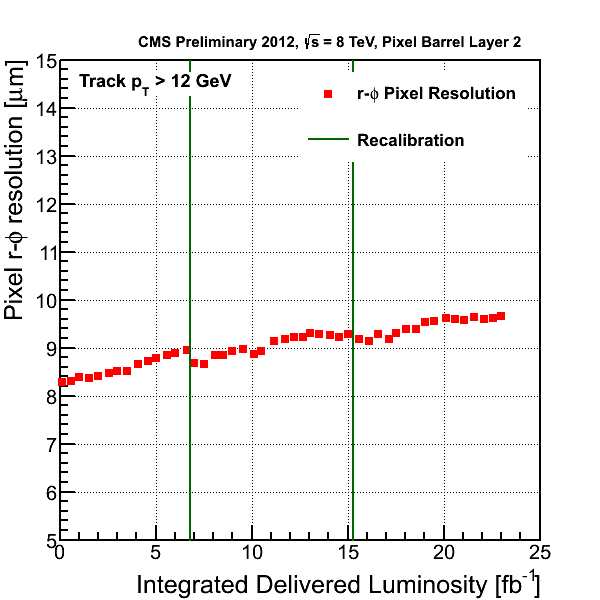
\includegraphics[width=0.48\textwidth]{figs/PXB2_residuals.png}
    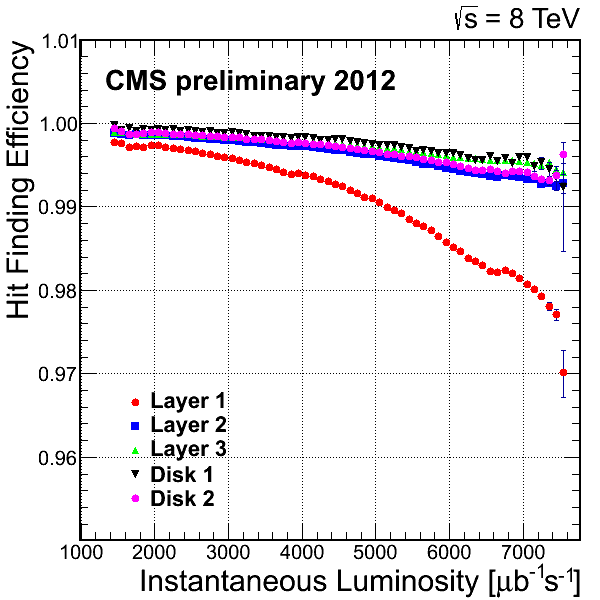
\includegraphics[width=0.48\textwidth]{figs/HitEff_vs_InstLumi.png}
    \caption{Resolution of the pixel detector in $r-\phi$ as function of the luminosity delivered to CMS detector [left] and efficiency of finding hits by the same detector [right]. The hit finding efficiency is higher than 98\% for the entire tracker. A degradation of pixel resolution is clearly visible as function of the recorded luminosity. A high hit finding efficiency is important for a precise \pt~measurement.}
    \label{fig:pixelresolution}
  \end{center}
\end{figure}

The Silicon Strip system is formed by an inner ($20\;\text{cm} < r < 55$ cm) and outer tracker ($55\;\text{cm} < r < 116$ cm). The inner tracker is composed of a 4-layer barrel (TIB for Tracker Inner Barrel) and 3 disks (TID for Tracker Inner Disks) in each endcap. The outer tracker systems is composed of 6 layers in the barrel (TOB for Tracker Outer Barrel) and 9 disks in each endcap (TEC for Tracker EndCap).

%The strips length is 10 cm with a pitch from 80 $\mu$m to 122 $\mu$m for single-sided strips and for 81 $\mu$m to 244 $\mu$m for double-sided. It's able to achieve a hit resolution of about 15 $\mu$m. 
%The MSGCs systems is composed of 6 layers in the barrel (TOB for Tracker Outer Barrel) and 11 disks in each endcap (TEC for Tracker EndCap, with a $\pm$ sign depending on the $z$ direction). Here the strips are 10 cm length for the inner layers and 25 cm for outer layers with a pitch from 200 $\mu$m to 400 $\mu$m, which gives a hit resolution of 35 $\mu$m and 100 $\mu$m respectively. The MSGCs and Silicon systems have an overall active area of around 300 $\text{m}^{2}$ with 12 $\times10^{6}$ channels organized in more than ten thousand independent modules.
%
%In figure~\ref{fig:cmstracker}, the disposition of all the tracker subsystems is shown. From the design of the tracker system the best resolution on the $p_{T}$ measurement is achieved in the $|\eta|<1.6$ region, this due to the presence of more layers of detector in the different subsystems, as shown in figure~\ref{fig:trackerres}. 

\begin{figure}[!Hhtbp]
  \begin{center}
    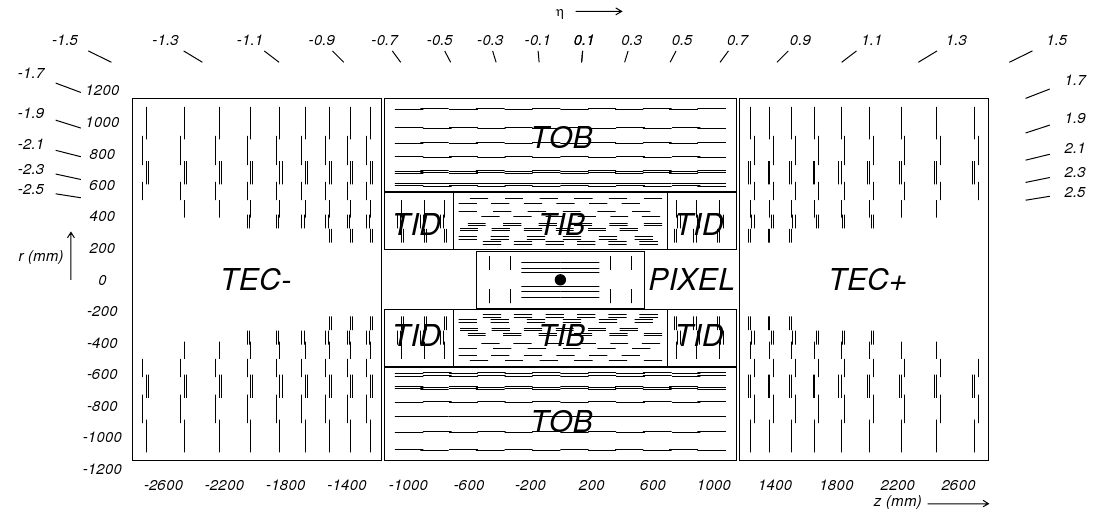
\includegraphics[width=0.9\textwidth]{figs/fig_cmstracker.png}
    \caption{CMS tracker system configuration: Pixel, Tracker Inner Barrel (TIB), Tracker Inner Disks (TID), Tracker Outer Barrel (TOB) and Tracker EndCap (TEC).}
    \label{fig:cmstracker}
  \end{center}
\end{figure}

\begin{figure}[!Hhtbp]
  \begin{center}
    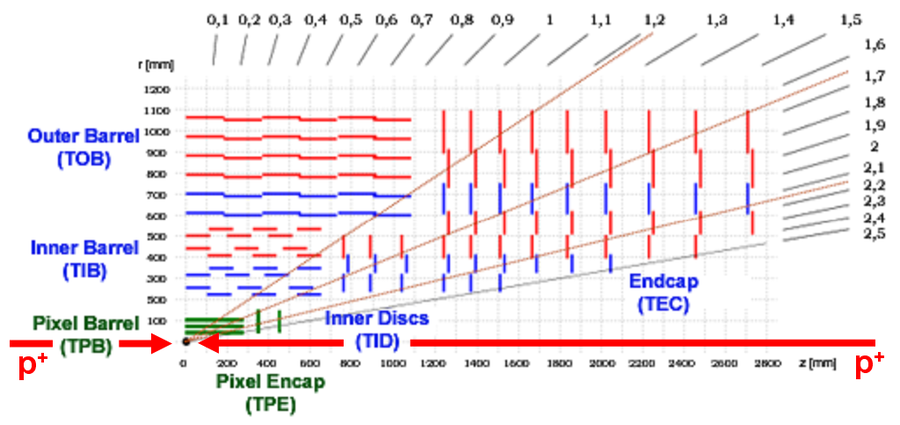
\includegraphics[width=0.9\textwidth]{figs/tracker_resolution.png}
    \caption{Tracker acceptance in $\eta$. }
    \label{fig:trackerres}
  \end{center}
\end{figure}

The tracker system has been designed to specifically address the reconstruction of high pt leptons, with particular interest in the isolation of electrons and, as a consequence, to isolate photons. This system reconstruct measures the energy of all electrically charged particles. Being charged hadrons the most important constituents of jets, the tracker plays a central role in their reconstruction. Also the tracker fulfills granularity requirements to reconstruct secondary vertexes to tag and reconstruct B-hadrons. The tracker system is able to reconstruct tracks of particles with at least 1 GeV of $p_{T}$ with $|\eta|<2.5$. Charged hadrons are reconstructed with an efficiency of at least 85\% for $p_{T}=1$ GeV and up to 95\% for $p_{T}$ above 10 GeV. Another important point that was taken into account is the fact that the tracker is the part of CMS most exposed to radiation as it is the closest subsystem to the interaction point. The tracker system was built highly resistant to radiation damage and is expected to last for around 10 years. %The pixel detector only lasts 2 years and was replaced during LS1. 

\subsection{Electromagnetic calorimeter}
\label{sec:ecal}

The CMS ECAL (Electromagnetic CALorimeter) is the detector subsystem designed to stop photons and electrons in order to measure their energy. It is an hermetic cylindrical calorimeter made of 61200 crystals in the barrel ($|\eta|<1.479$) and 7324 in each endcap ($1.48<|\eta|<3$). The crystals material is lead-tungstate that is transparent, very dense (8.28 g/$\text{cm}^{3}$), has a small Moliere radius (2.2 cm) and a short radiation depth ($X_{0}=0.89$ cm). This material has been chosen for the characteristics already described, but also because of its fast emitting scintillation light (about 25 ns) and its good energy resolution, typically with $\sigma(E)/E\sim 0.05$\% for an energy of 50 GeV and $\sigma(E)/E\sim 0.04$\% for an energy of 100 GeV . The main disadvantage of this material is its high dependent response to the temperature (about 2\% /\celsius), making crucial to maintain a stable temperature in the ECAL system. The crystals are distributed in 36 super-modules, 1700 crystals each, in the barrel (EB for ECAL Barrel) and in four 'Dee's, of 3662 crystals each, in the endcaps (EE for ECAL endcap). In the EB the scintillation light is collected by Avalanche Photo-Diodes, or APD, and by Vacuum Photo-Triodes, or VPT, in the EE. A preshower system is installed in front of each endcap to allow a better discrimination between photons and $\pi^{0}$'s. A representation of the CMS ECAL can be found on figure~\ref{fig:ecal}.

\begin{figure}[!Hhtbp]
  \begin{center}
    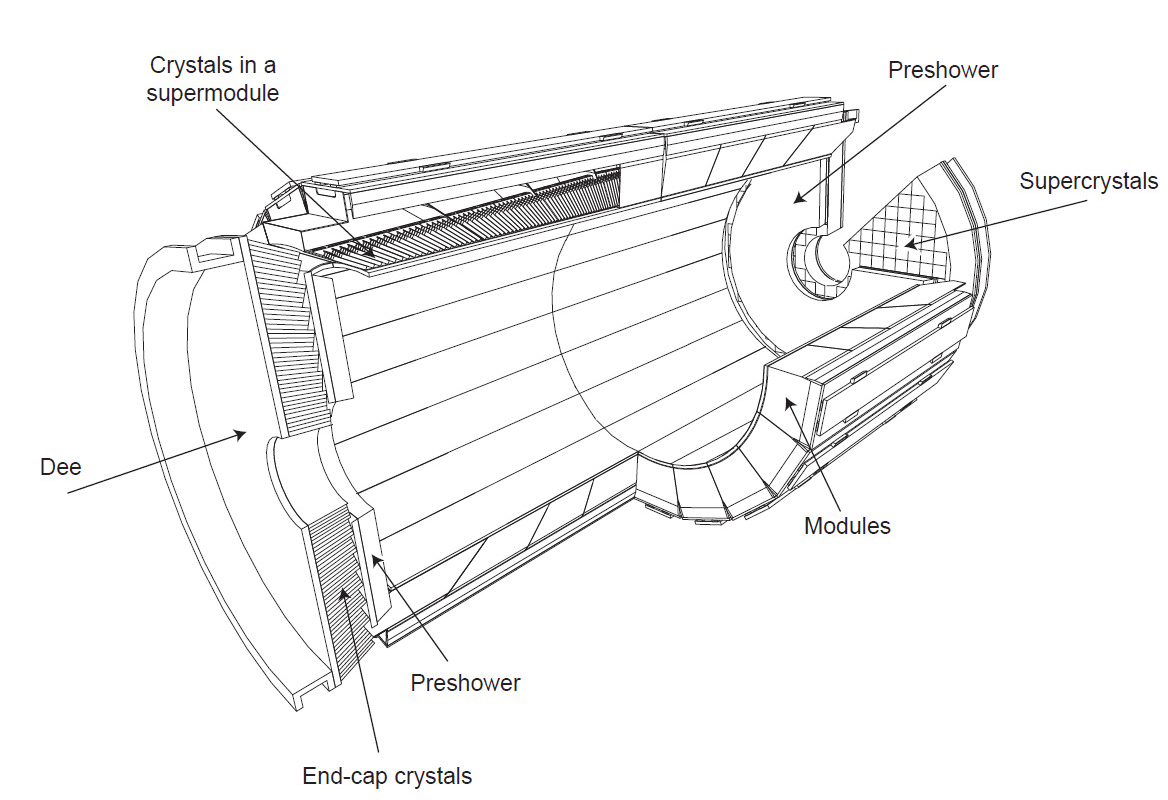
\includegraphics[width=0.9\textwidth]{figs/ECAL.png}
    \caption{CMS ECAL representation showing its different components: barrel modules, the preshower system and endcap 'Dee's.}
    \label{fig:ecal}
  \end{center}
\end{figure}

The ECAL system requires constant correction to the loss of transparency due to aging by radiation. Figure~\ref{fig:RelaResp} shows the relative response of the crystals during LHC run 1 and the di-electron mass from electrons measured in the ECAL barrel, taken from~\cite{CMS-DP-2012-015}. The aging of the crystals is measured by a laser monitoring system that measures the transparency of the crystals. To validate the corrections derived from the laser monitoring a comparison is performed between the reconstruction of electrons by the tracker and the ECAL. Such comparison in function of time can be seen in figure~\ref{figs:RelEp} (from~\cite{CMS-DP-2012-015}).

\begin{figure}[!Hhtbp]
  \begin{center}
    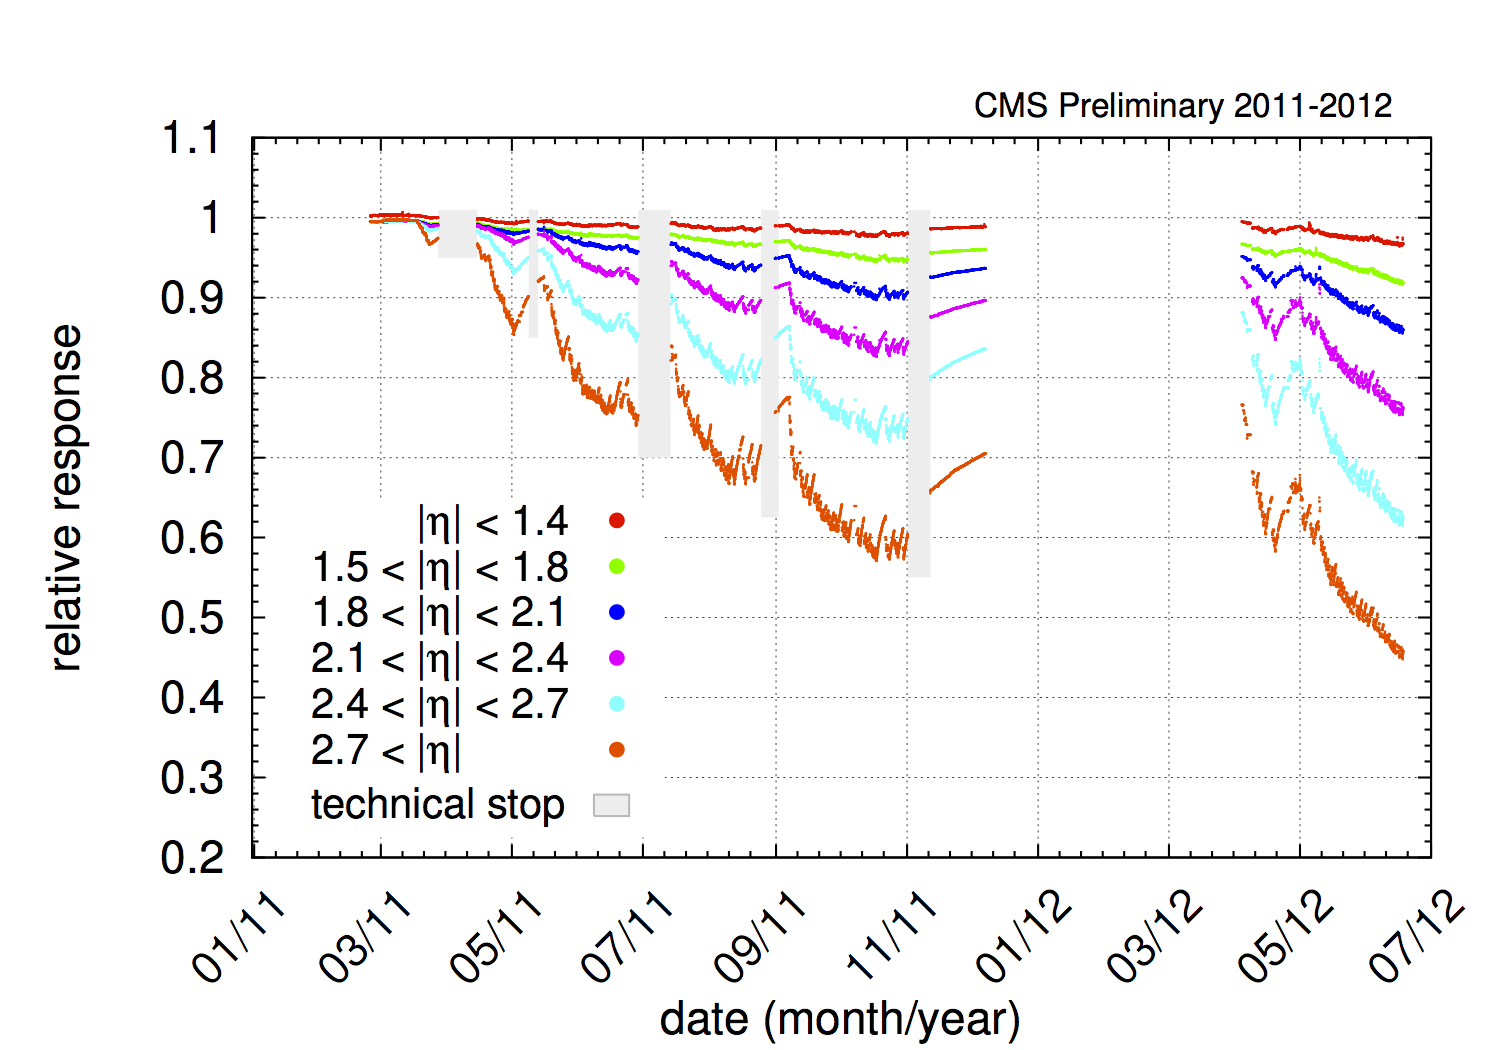
\includegraphics[width=0.48\textwidth]{figs/laser_monitoring_histories_2011-2012.png}
    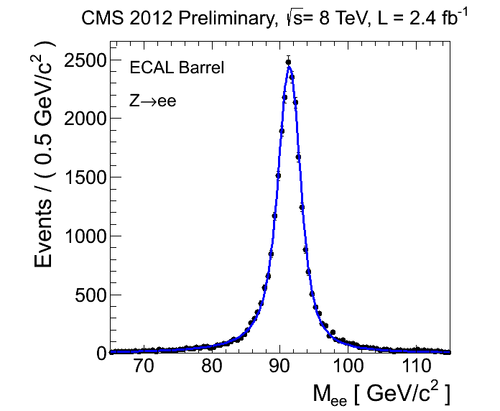
\includegraphics[width=0.48\textwidth]{figs/_500___2012_zee_eb_golden.png}
    \caption{Relative response of the ECAL crystals as function of time, for different $\eta$ regions [left]. Di-electron invariant mass from electrons identified in the ECAL barrel [right].}
    \label{fig:RelaResp}
  \end{center}
\end{figure}

\begin{figure}[!Hhtbp]
  \begin{center}
    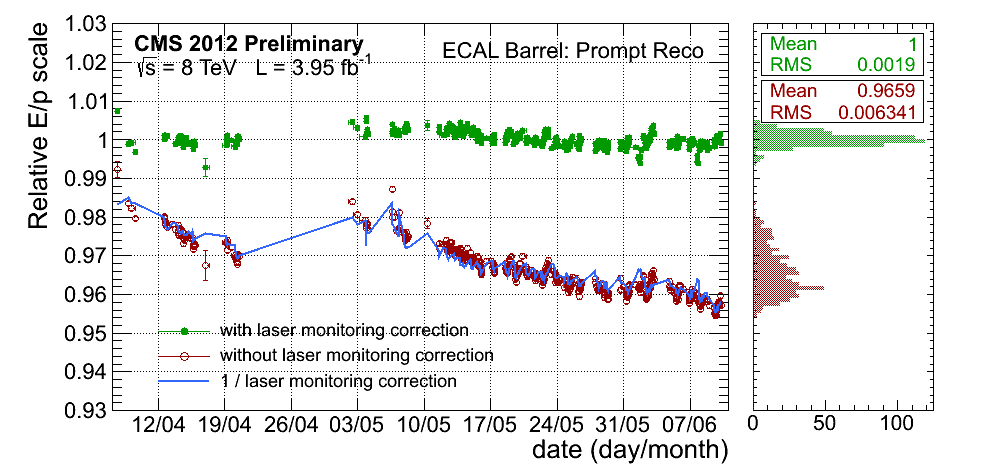
\includegraphics[width=0.9\textwidth]{figs/EoverP_history_2012.png}
    \caption{Relative $E/p$ for electrons with and without laser monitoring as function of time. The electron energy $E$ is measured by the ECAL while its momentum $p$ is measured using the tracker information. Laser monitoring is able to effectively correct ECAL lost of transparency.}
    \label{figs:RelEp}
  \end{center}
\end{figure}

%\begin{TOINCLUDE}Plot on crystal response, dielectron reconstruction on the ECAL, ratio of E/p for reconstructed electrons E from the ECAL and p from the tracker\end{TOINCLUDE}

\subsection{Hadronic Calorimeter}
\label{sec:hcal}

The CMS HCAL, for Hadronic CALorimeter, is the subdetector designed to measure the energy of hadrons produced in the collisions. It is an hermetic set of subsystems covering up to $|\eta|<5.2$:
\begin{itemize}
\item Hadron Barrel Calorimeter (HB): Covering $|\eta|<1.4$ is located between the ECAL barrel and the magnet. 
\item Hadron Endcap Calorimeter (HE): Extends the coverage of the barrel on the region $1.4<|\eta|<3$.
\item Hadron Outer Calorimeter (HO): Located outside the magnet, uses it as an additional absorber.
\item Hadron Forward Calorimeter (HF): Completes the coverage of the system from $|\eta|=3$ up to $|\eta|=5.2$.
\end{itemize}

The CMS HCAL layout is shown in figure~\ref{fig:hcal}. The system is made of two parts, an absorber to develop the hadronic showers and a scintillator to measure the particles energy. The length scale of hadronic calorimetry is defined as the interaction length corresponding to the mean free path of an hadron in a material. The typical length of an hadronic shower is around 300 mm. The HB absorber is made of 40 mm thick steel plate, eight layers of brass plates of 50.5 mm thick, six brass plates of 56.5 mm thick and a steel plate of 75 mm thick. The HE uses the same absorber but with thicker plates, of 79 mm. Between the absorber plates a plastic scintillator, Kuraray SCSN81, 3.7 mm thick, is placed. In the region with $|\eta|<1.6$ the achieved granularity is $\Delta\eta\times\Delta\phi=0.087\times 0.087$ and $\Delta\eta\times\Delta\phi=0.17\times 0.17$ in the region with $|\eta|>1.6$. This design gives a total of 70000 tiles. The produced light in the HB is collected by optical fibers and transferred to the Hybrid Photo Diodes (HPDs). These diodes were chosen thanks to their small sensitivity to the magnetic field, an important feature because HCAL is inside the solenoid magnet. %due to the proximity of the HCAL to the magnet.

\begin{figure}[!Hhtbp]
  \begin{center}
    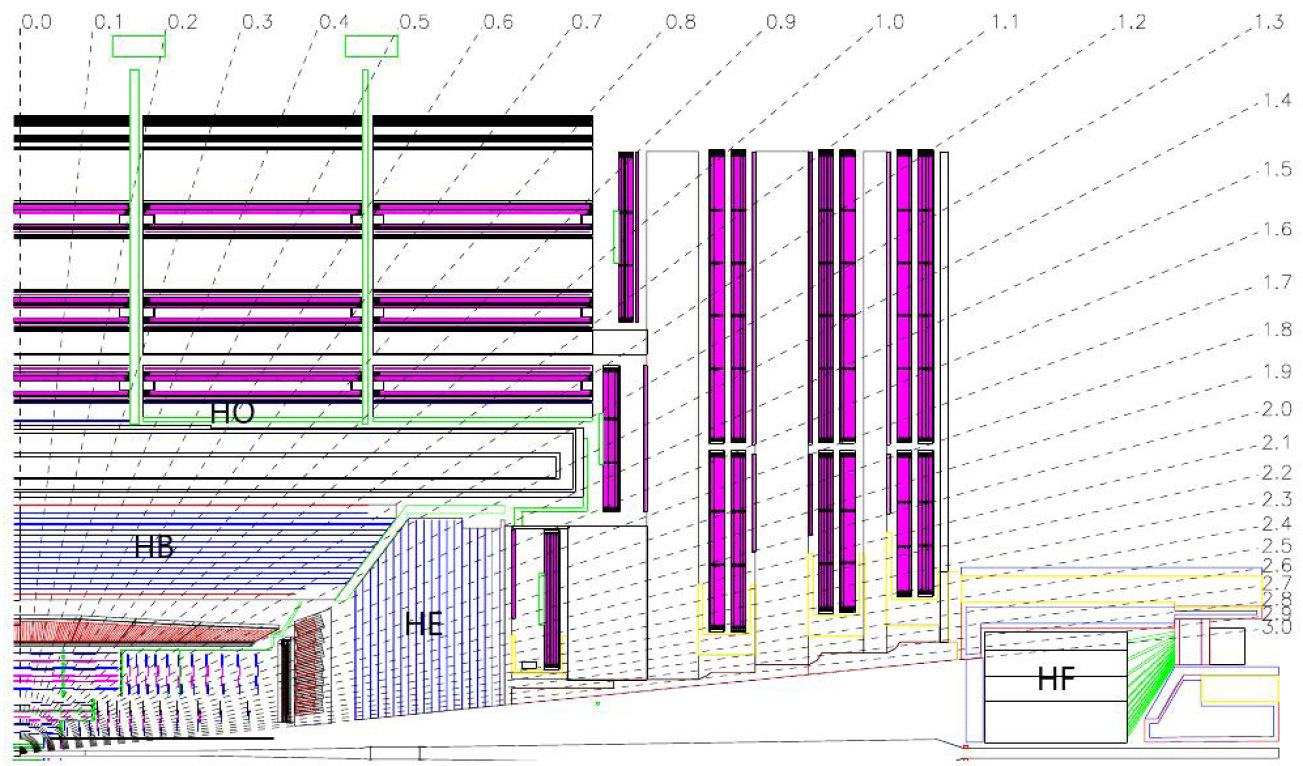
\includegraphics[width=0.9\textwidth]{figs/HCAL.png}
    \caption{CMS HCAL representation. }
    \label{fig:hcal}
  \end{center}
\end{figure}

The HF design is very different from the rest of the HCAL subsystems. The most important challenge for the HF is the high resistance to radiation, while in the central rapidity region 100 GeV are deposited in average in the forward region is 760 GeV. For this reason a Cherenkov detector made of quartz fibers with a steel absorber was chosen. The light produced in the HF is collected by photo multipliers. 

HCAL response is defined as the energy measured by it with respect to the momentum of a track, being measured by the tracker system, for a single particle. In the most central region, $|\eta|<0.52$, the HCAL response is $\sim$ 0.6 for ${p_{Track}>8\;\text{GeV/c}}$. In the region $1.39<|\eta|<2.01$ the response is $\sim$ 0.4 for ${p_{Track}>8\;\text{GeV/c}}$.

%In figure~\ref{fig:hcal_per} can be seen the HCAL response to a single track as function of its momentum, characterizing the energy seen by the HCAL from a single particle respect to its true energy.
%
%\begin{figure}[!Hhtbp]
%  \begin{center}
%    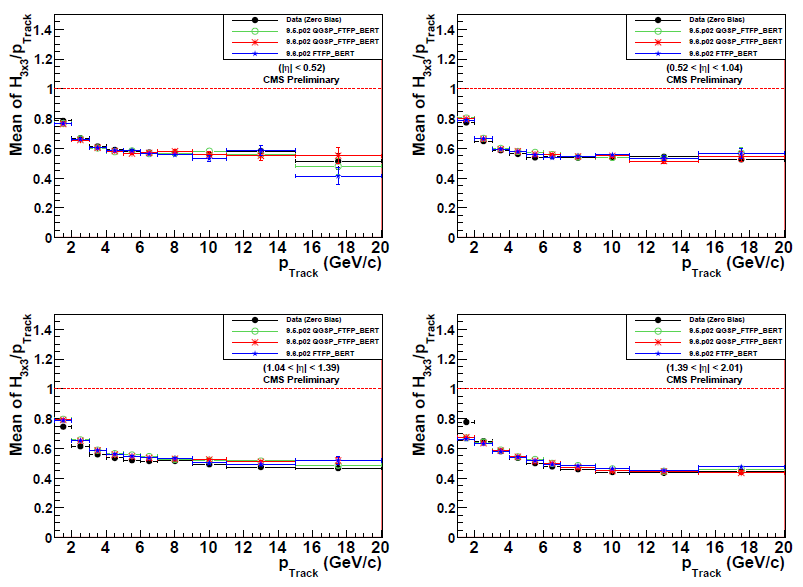
\includegraphics[width=0.9\textwidth]{figs/HCAL_perf.png}
%    \caption{Mean response measured in the 3 $\times$ 3 tower matrix of the HCAL as a function of track momentum
%being compared with the predictions of three sets of Monte Carlo for different $\eta$ regions}
%    \label{fig:hcal_per}
%  \end{center}
%\end{figure}

Calorimeters, ECAL and HCAL, and tracker are the fundamental pieces to identify the hadronic products of collision events. Whereas HCAL is designed to measure the energy of hadrons produced from collisions, but its information alone its not sufficient to correctly reconstruct them. We will discuss how the calorimeters information is combined to reconstruct physics objects called jets in section~\ref{sec:jets}.

\subsection{Muon chambers}
\label{sec:muons}

The muon system of CMS is located at the most exterior layer of the detector  due to the penetration power of this particle. Muons are not stopped by the calorimeters and, with neutrinos, they are able to escape the detector. The muon chambers are placed in a cylinder around the HO and in disks on the endcaps. Three main characteristics have been fulfilled from the design: efficient muon identification, precision measurement of muon charge and momentum, and fast measurement to provide trigger capabilities. These chambers are made of three different subsystems:
\begin{itemize}
\item Drift Tubes Chambers (DT): Located in the region with $|\eta|<1.2$ and disposed in four layers. They consist of individual drift tubes of 50 $\mu$m of diameter anode wire with two electrode plates creating a drift electric field. The wall of the cell act as cathode. The cells are filled with a gas mixture, 85\% Argon and 15\% $\text{CO}_{2}$. The tubes are organized in plaques that are also organized in SuperLayers (SL) each one made of 4 plaques. The barrel is made of 250 DT's disposed in four cylinders separated by iron yokes. 
\item Cathode Strip Chambers (CSC): Installed in the endcaps, provide a coverage up to $|\eta|=2.4$ from $|\eta|=0.9$. These chambers are multi-wire proportional chambers made of six planes of anode wires with 7 cathode planes. Four CSC stations are placed in each endcap. The wires are oriented in azimuthal direction while the cathode planes are radially oriented, allowing a complete measurement of the particle position. This system is able to measure with a precision between the 75 $\mu$m and 150$\mu$m.
\item Resistive Plate Chambers (RPC): This subsystem is made of gaseous parallel plate detectors. This detector is specially useful for triggering as it is very fast and have a good position resolution. There are 480 RPC distributed in 6 layers in the barrel with the DT and in 3 layers in the endcaps with the CSC, and covers the region with $|\eta|<1.6$. 
\end{itemize}

Figure~\ref{fig:cmsmuon} shows a representation of the muon system with the different components. The DT and CSC system cover $|\eta|<2.4$ without any gap. 

\begin{figure}[!Hhtbp]
  \begin{center}
    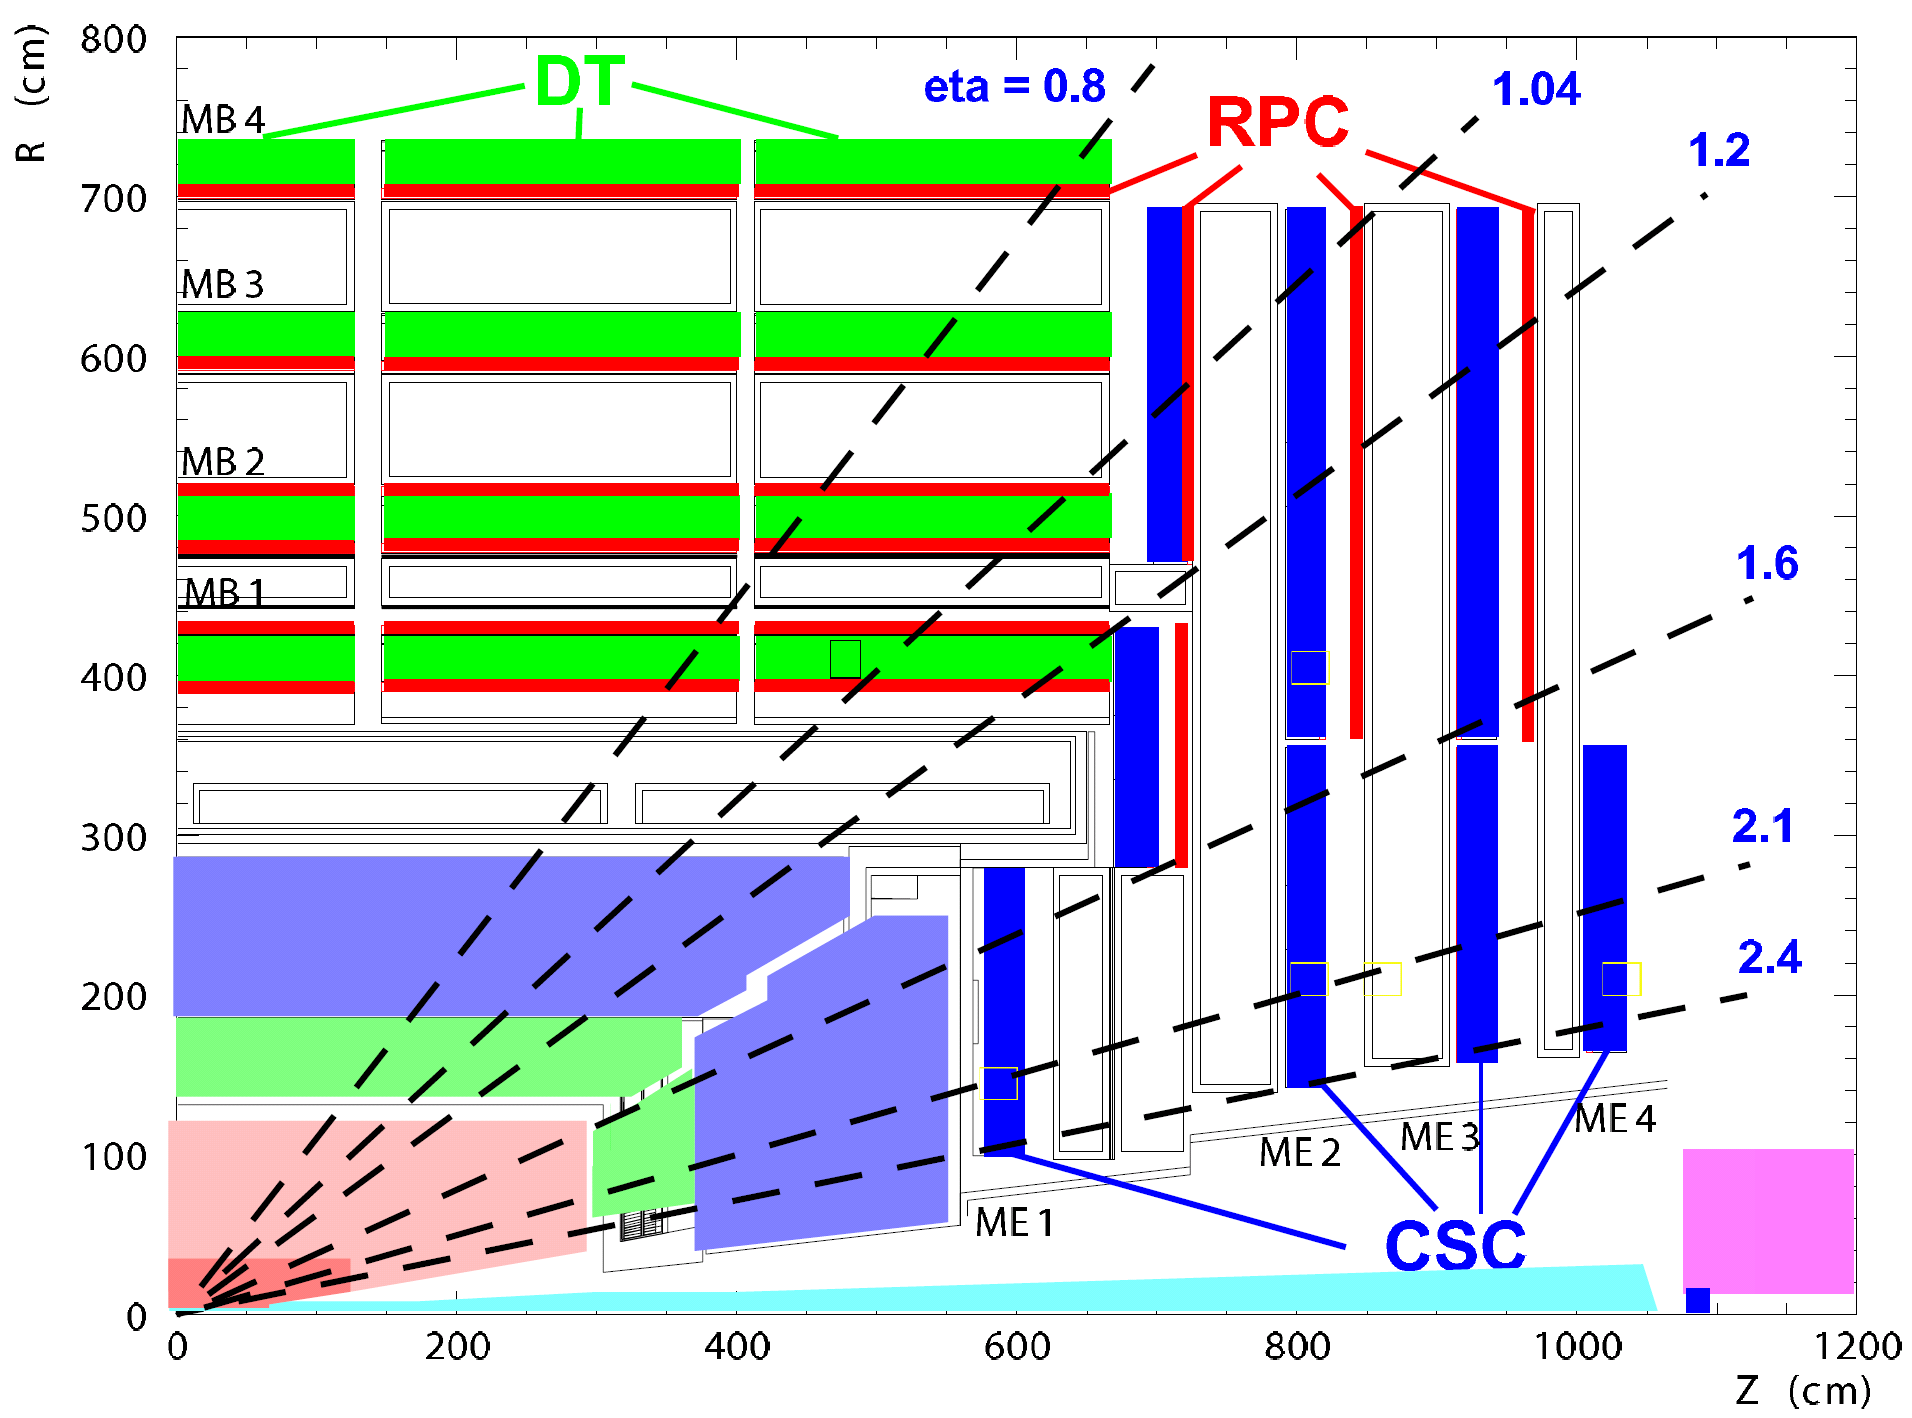
\includegraphics[width=0.9\textwidth]{figs/MuonDetector.png}
    \caption{CMS muon chambers representation. }
    \label{fig:cmsmuon}
  \end{center}
\end{figure}

Information from DT, CSC and RPC subsystems are utilized to reconstruct muons in CMS detector. In figure~\ref{fig:MuonEff} the muon reconstruction efficiency for the three subsystems~\cite{Chatrchyan:2013sba} is shown.  

\begin{figure}[!Hhtbp]
  \begin{center}
    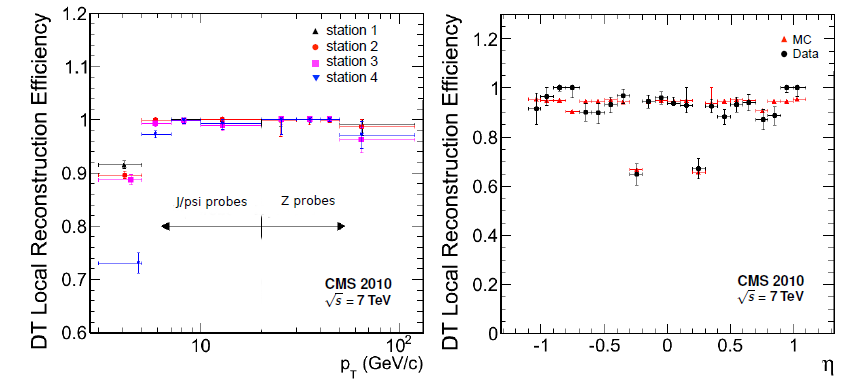
\includegraphics[width=0.9\textwidth, height=0.3\textheight]{figs/DT_Eff.png}
    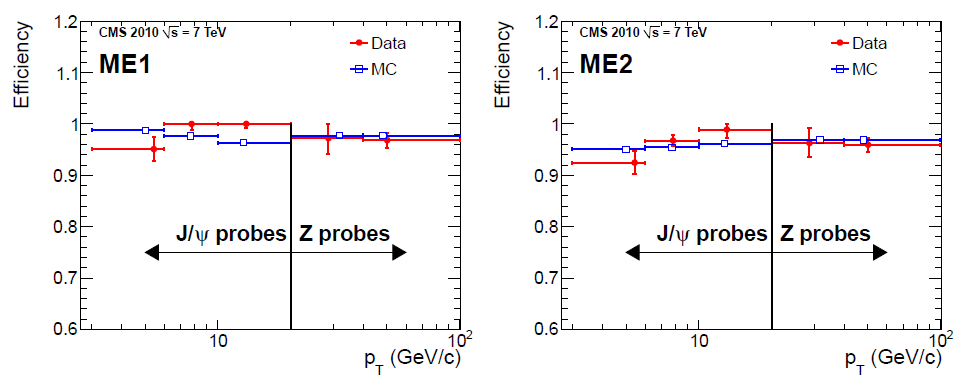
\includegraphics[width=0.87\textwidth, height=0.3\textheight]{figs/CSC_Eff.png}
    %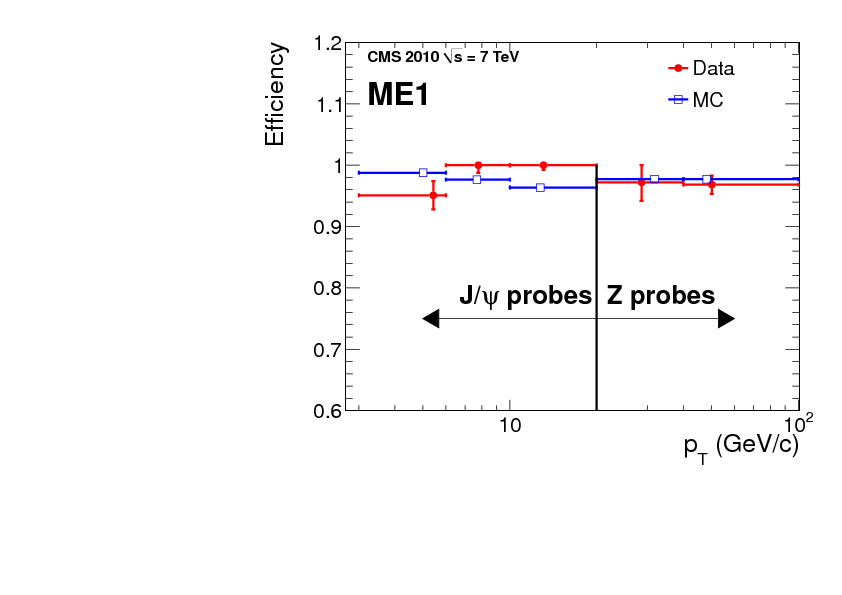
\includegraphics[width=0.45\textwidth, height=0.3\textheight]{figs/Sections_EfficiencyFigs_CombPtEff_Station1_TPDataMC_Active_CSC.png}
    %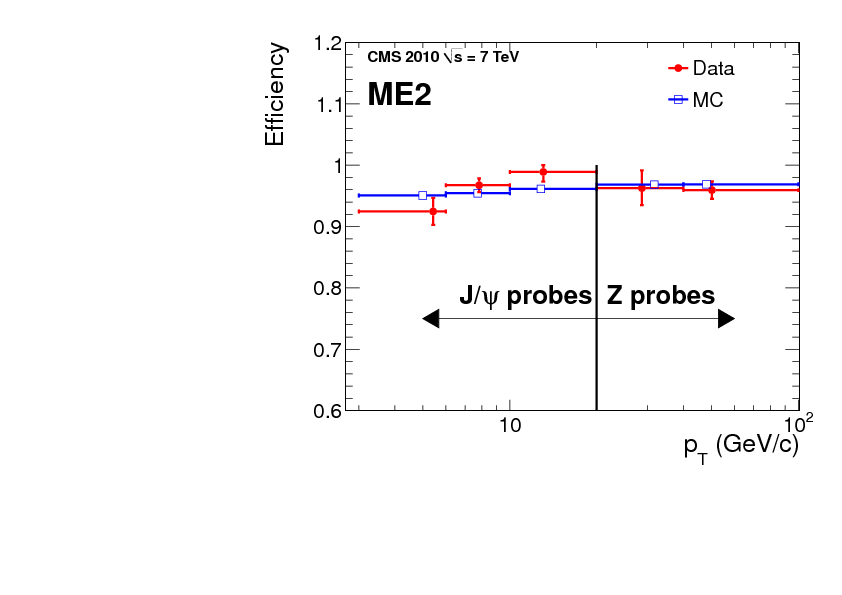
\includegraphics[width=0.45\textwidth, height=0.3\textheight]{figs/Sections_EfficiencyFigs_CombPtEff_Station2_TPDataMC_Active_CSC.png}
    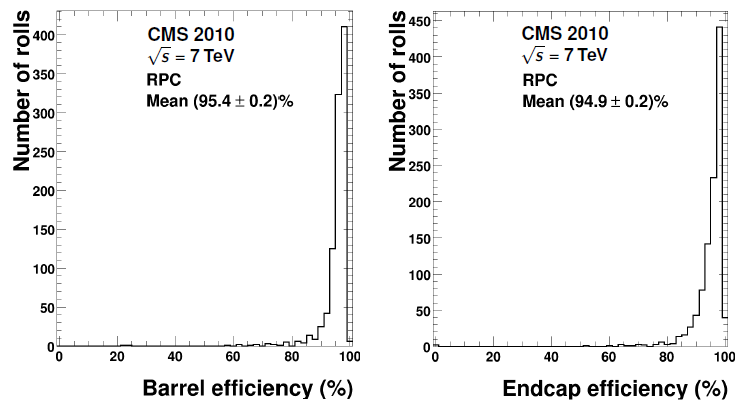
\includegraphics[width=0.86\textwidth, height=0.3\textheight]{figs/RPC_Eff.png}
    \caption{Muon reconstruction efficiency in the 4 barrel DT stations as function of $p_{T}$ and $\eta$ [up], muon reconstruction efficiency for data and Monte-Carlo simulation as function of $p_{T}$ for the two CSC end-cap stations [middle], muon reconstruction efficiency for RPC barrel and end-cap [down].}
    \label{fig:MuonEff}
  \end{center}
\end{figure}

%The RPC subsystem efficiency depends on the voltage used and in the pressure of the injected gas. The efficiency on the RPC barrel during the run I data taking can be seen in figure~\ref{fig:RPCBarrelEff}.
%
%\begin{figure}[!Hhtbp]
%  \begin{center}
%    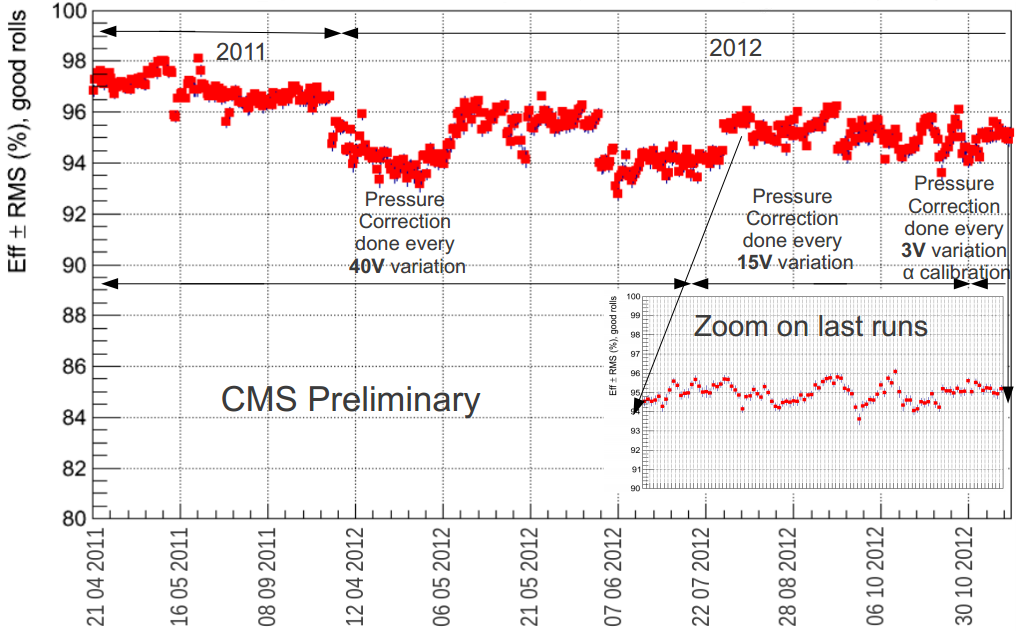
\includegraphics[width=0.9\textwidth]{figs/HistPlot2011_2012_EffBarrel.png}
%    \caption{RPC Barrel efficiency during two years of data taking}
%    \label{fig:RPCBarrelEff}
%  \end{center}
%\end{figure}
%
%\begin{TOINCLUDE}Plot of RPC efficiency during Run1 and L1 RPC efficiency as function of probe PT\end{TOINCLUDE}
%
\subsection{Trigger}
\label{sec:trigger}

LHC has been designed to collect data from proton-proton collisions every 25 ns, meaning a frequency of 40 MHz. Each recorded event by CMS has a nominal size between 0.5 and 1 MB, corresponding to a data flow of around $10^{9}\; \text{MB/s}= 1\text{PB/s}$ that is extremely big for transfer and for storing. Therefore, an on-line selection of events has to be done. The trigger system of CMS does this task in two fold, a level 1 (L1) and a high level trigger (HLT). The L1 is hardware based and the HLT is software based. 

From the searches conducted at CMS, the interesting events produced on proton-proton collisions for new physics searches are very rare. The enormous majority of events coming from proton-proton collisions correspond to well understood phenomena, while new physics events are 'exotic' with regards to the most common type of events. Then it is interesting to keep only a part of the events, what actually makes easier the analyses afterward done over the data. 

The CMS trigger system is designed to keep only 100 kHz by the L1 and 1 kHz by the HLT. L1 is reducing the data flux by 2 orders of magnitude and the HLT another 3 orders of magnitude.
%
%During data taking or in general CMS operation the trigger system needs to be constantly supervised in order to guarantee the quality of collected data. For this purpose, a person is always looking that the whole trigger system has no failures, in particular that the data collection frequency do not overflow. During my second year of my doctorate, I did some of these trigger shifts during different detector tests to take data from cosmic rays as preparation for run 2. %From the trigger performance depend the quality of the collected data. 

\subsubsection{Level 1 trigger}
\label{sec:L1}

The L1 is designed to trigger over coarse data coming from the calorimeters and muon chambers, holding data in pipe-lined memories in the front-end electronics. Therefore, it relies on very fast reconstruction of objects coming from this subsystems: muons, electrons, photons, jets and missing energy (summing up \HT~and $M_{H_{T}}$). This reconstruction differs from the final reconstruction of the objects, that has a smaller granularity. For example a jet for the L1 consists on successive energy deposits in the ECAL and HCAL, while the off-line reconstruction takes into account also the tracker information. 

The L1 starts from regional data coming from the subsystems which is afterward combined in order to build ranked trigger objects in localized regions of the detector. Global Muon and Calorimeter triggers sort the objects and send the best ranked to the Global Trigger (GT). Before the GT no events are rejected, it is only with the GT that the selection is applied. The GT combines the information and can apply topological requirements and take a decision on keeping or disregarding the event. On figure~\ref{fig:l1} the work-flow of the L1 is shown, taken from~\cite{Lenzi:2013xpa}. 

\begin{figure}[!Hhtbp]
  \begin{center}
    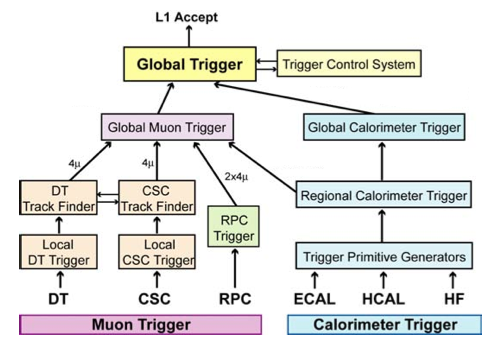
\includegraphics[width=0.9\textwidth]{figs/img_l1.png}
    \caption{L1 architecture.}
    \label{fig:l1}
  \end{center}
\end{figure}

The L1 cards are distributed between the detector and a nearby cavern at 7 m distance from the detector. The latency time that the L1 disposes between the collision and the taking of the decision is about 3.2 $\mu$s. Therefore, the front-end memory in the cards should be able to keep in memory up to 128 bunch crossings. 

\subsubsection{High Level Trigger}
\label{sec:HLT}

%The HLT takes as input the events accepted by the L1 and processes them using farms of commercial processors. The HLT does additional operations on the selected events making it much slower than L1 processing. In particular, the HLT takes also into account the tracker information. Consequently, this system is able to take into consideration the whole information of the detector. However, the reconstruction of objects done by the HLT differs slightly from the final off-line reconstruction. The decision taking process takes around 40 ms, $10^{4}$ times more than for L1. 

Events passing the L1 pass to the High Level Trigger (HLT), a set of filtering algorithms that run in CPU farms of about $10^{4}$ cores. The reconstruction of objects done by the HLT differs slightly from the final off-line reconstruction. Final off-line reconstruction takes into account the whole information of the detector following the procedure described in section~\ref{sec:reco}, while reconstruction for the trigger do a simpler procedure due to computing time limitations. During 2012, the decision taking process was 110 ms, around $10^{5}$ times more than for L1.

HLT is divided in several paths, where each path correspond to a specific filtering algorithm. Each path contributes with a rate to the HLT, such that the sum of the rates of all path sum up the total HLT rate. The events selected by HLT are finally stored on disks under several paths depending on the selection performed. There is a constant development of HLT paths focusing on different analysis requirements in order to obtain the best possible selection efficiency for specific signal types. 

\section{Object reconstruction}
\label{sec:reco}

The different subsystems of CMS play specific roles in the identification of particles from collisions and measurement their properties. In order to achieve such measurements, the information collected by the different parts of a subsystem should be combined. Also, for some particles, the information between different subsystems should be connected to achieve a successful identification.% The easiest example is the reconstruction of tracks in the pixel detector. In order to identify a track of a charged particle that traversed the pixel barrel the hits of such particle in each layers should be considered at the same time. A track in the pixel barrel is formed then by the three hits a particle leaves in each barrel layer.

\subsection{Particle Flow (PF) algorithm}

CMS uses a sophisticated algorithm called Particle flow~\cite{CMS:2009nxa,CMS:2010eua,CMS:2010byl,CMS:2010aua} to reconstruct the particles detected in the subsystems: charged and some neutral hadrons, electrons, muons and photons. The algorithm uses the information from all the subsystems to ameliorate the reconstructed objects resolution.% The PF is specially important for the reconstruction of jets, using the tracker information to overpass the HCAL weaknesses. 
The quality of the objects reconstructed by this algorithm greatly affects the analyses, as they rely in the information of these objects. The Particle flow algorithm has been optimized to give the best performance in terms of minimal fake rate, correct energy and momenta reconstruction. Precisions will be given later, when the objects will be described.

\subsection{Track and vertex reconstruction}

A vertex is defined as the point from where several tracks in the detector are originated. Reconstruction of vertices and tracks is one of the most important parts of the reconstruction of events. The identification of the primary vertex of an event is crucial to separate objects coming from a hard interactions from other interactions, as pile up. The primary vertex reconstruction is performed by clustering tracks together and performing fits to determine the likelihood these tracks originated from a common vertex. The reconstructed vertex with the largest total \pt~is considered the primary vertex.

Track reconstruction proceeds from the clustering of pixel and silicon strips signals into hits. The found hits in the different layers of the tracker are used to reconstruct the trajectory of the charged particle that left the hits. In order to reconstruct trajectories, at least three hits or two hits and a vertex constraint are needed. The reconstruction proceeds from the propagation of hits in different layers. This process could lead to multiple possible tracks, in order to discard fake tracks and to choose the most likely tracks the vertex compatibility and the number of hits per tracks are used. Most compatible tracks and with the highest number of hits are preferred. Finally, a $\chi^{2}$ fitting is used in order discriminate between multiple tracks. 

A way to estimate the goodness of the reconstruction is to measure the reconstruction efficiency of charged pions and muons, such efficiencies are shown in figure~\ref{fig:TrackerEff}, taken from~\cite{Chatrchyan:2014fea}. The reconstruction is near 100\% efficient for muons and pions with $p_{T}>$ 1 GeV. Vertex reconstruction proceeds from clustering of tracks.

\begin{figure}[!Hhtbp]
  \begin{center}
    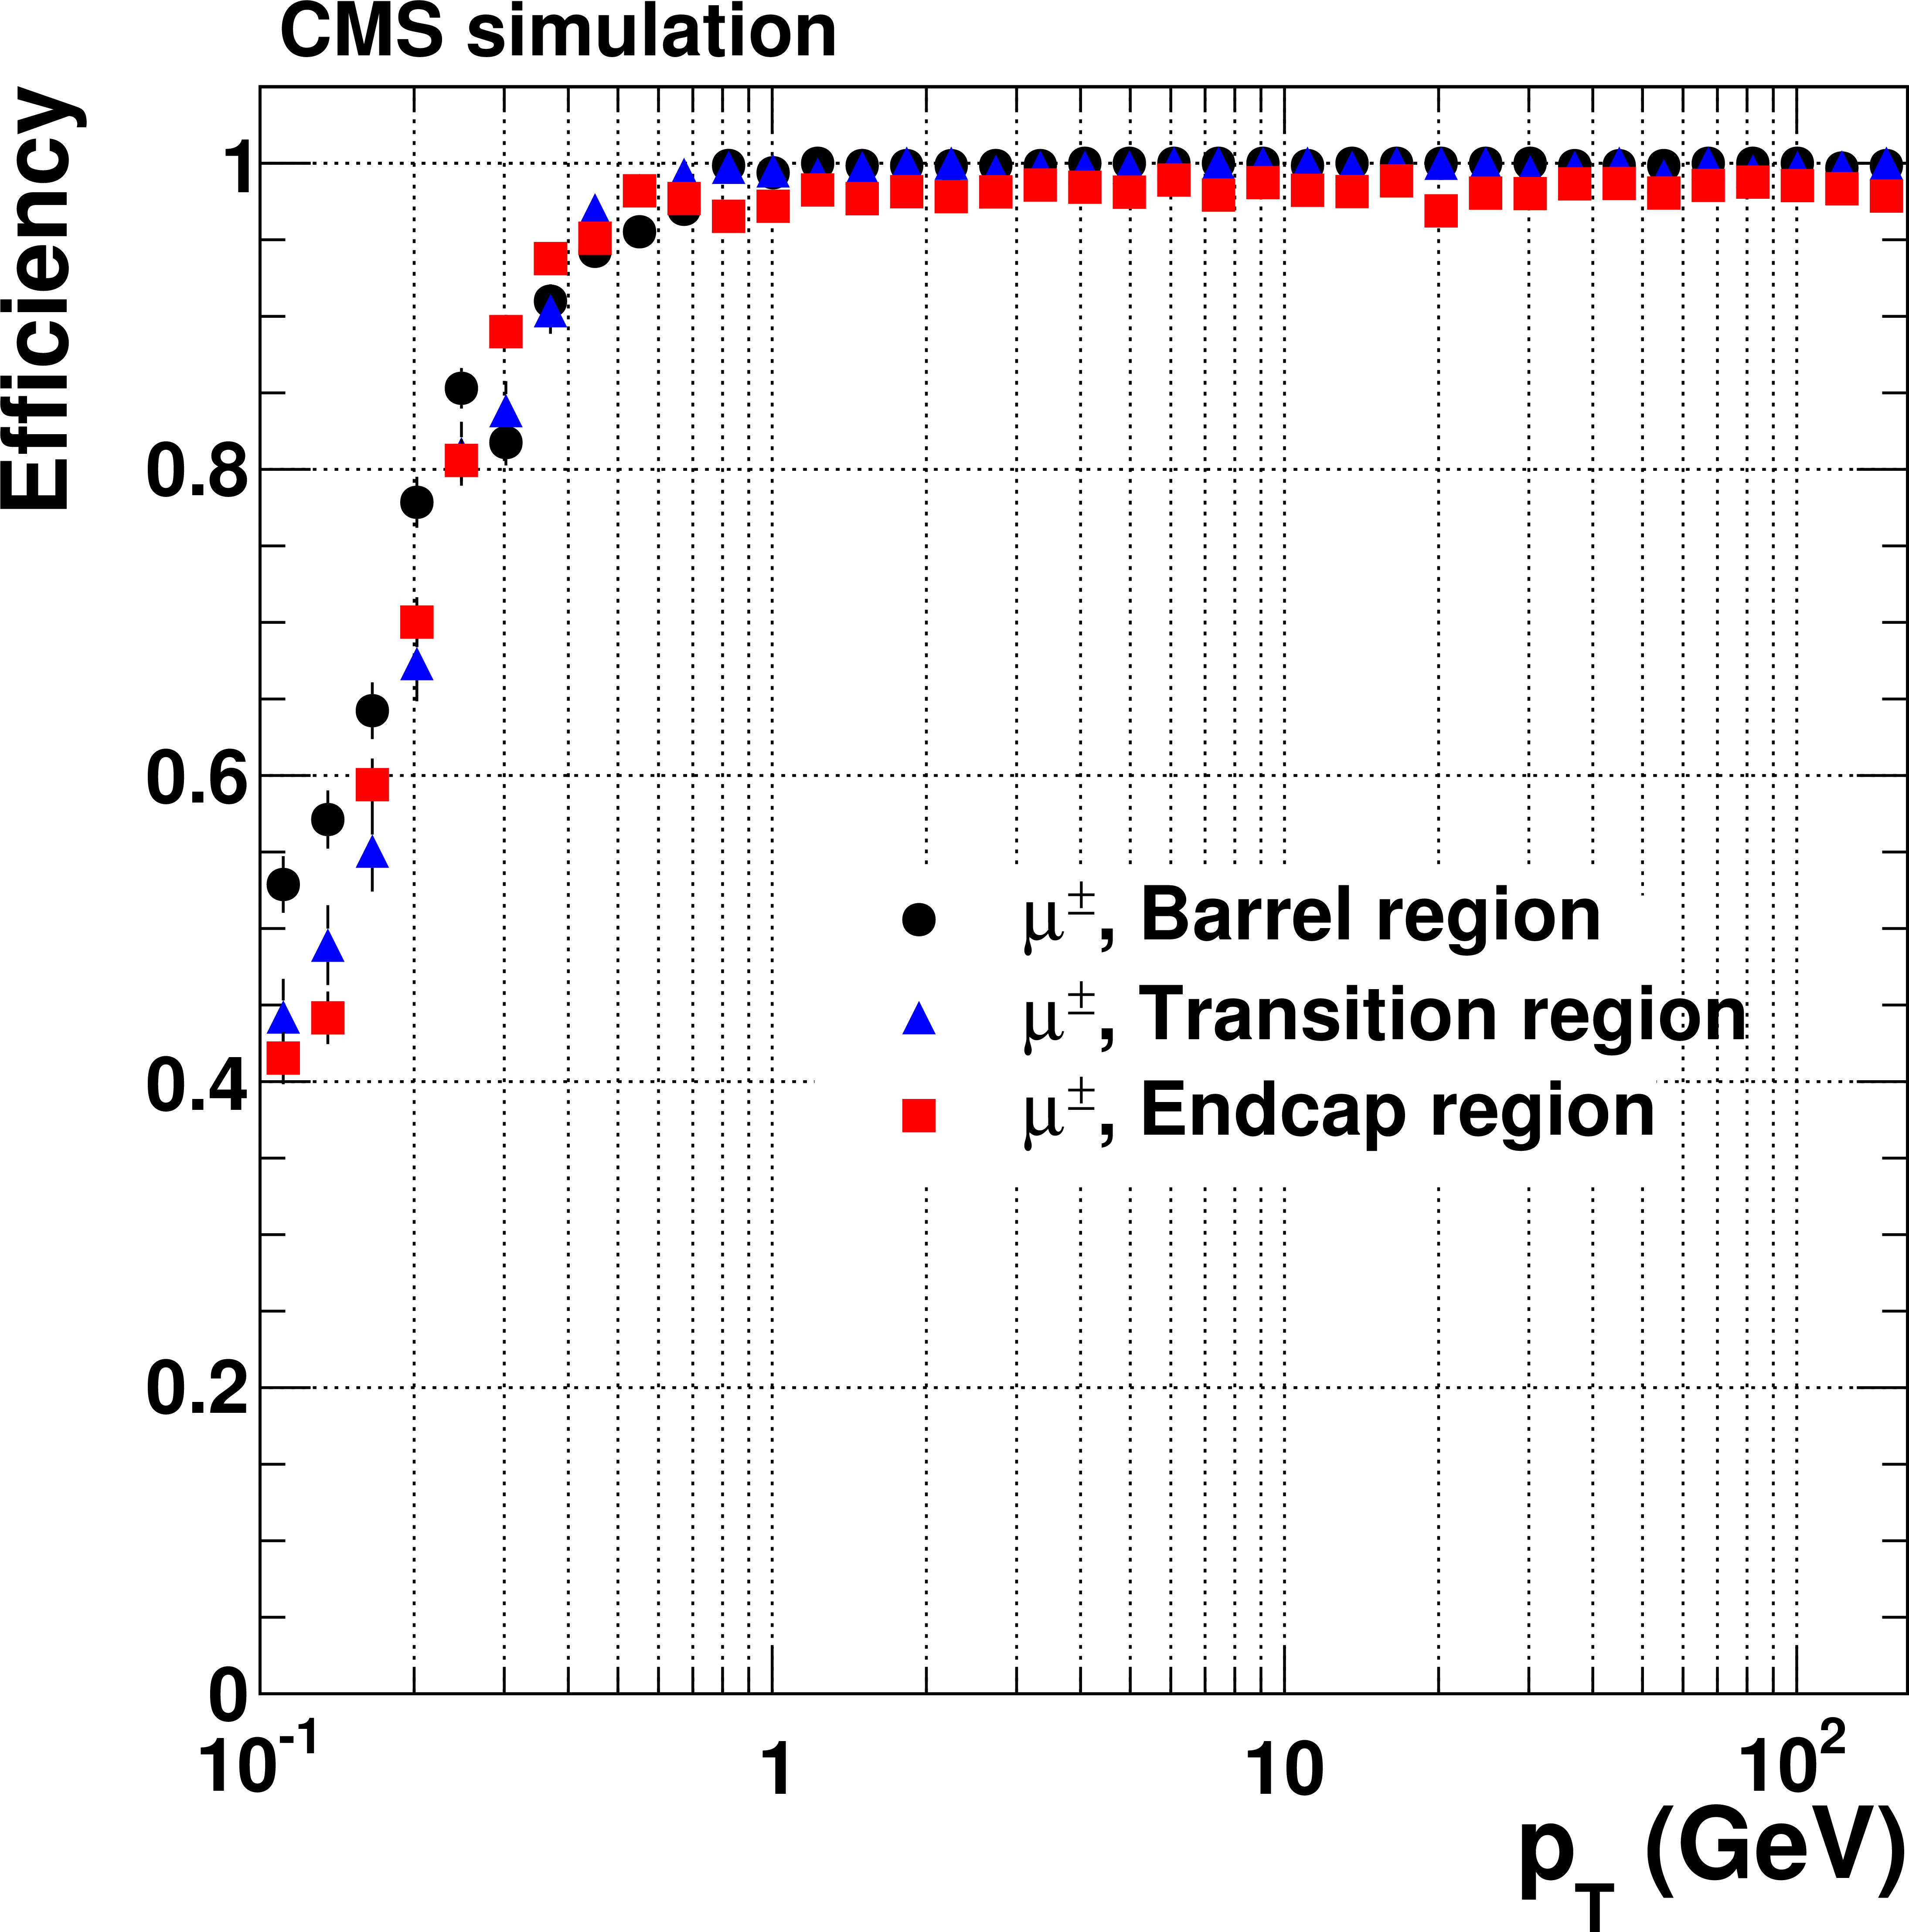
\includegraphics[width=0.45\textwidth]{figs/eff_muon_vs_pt.png}
    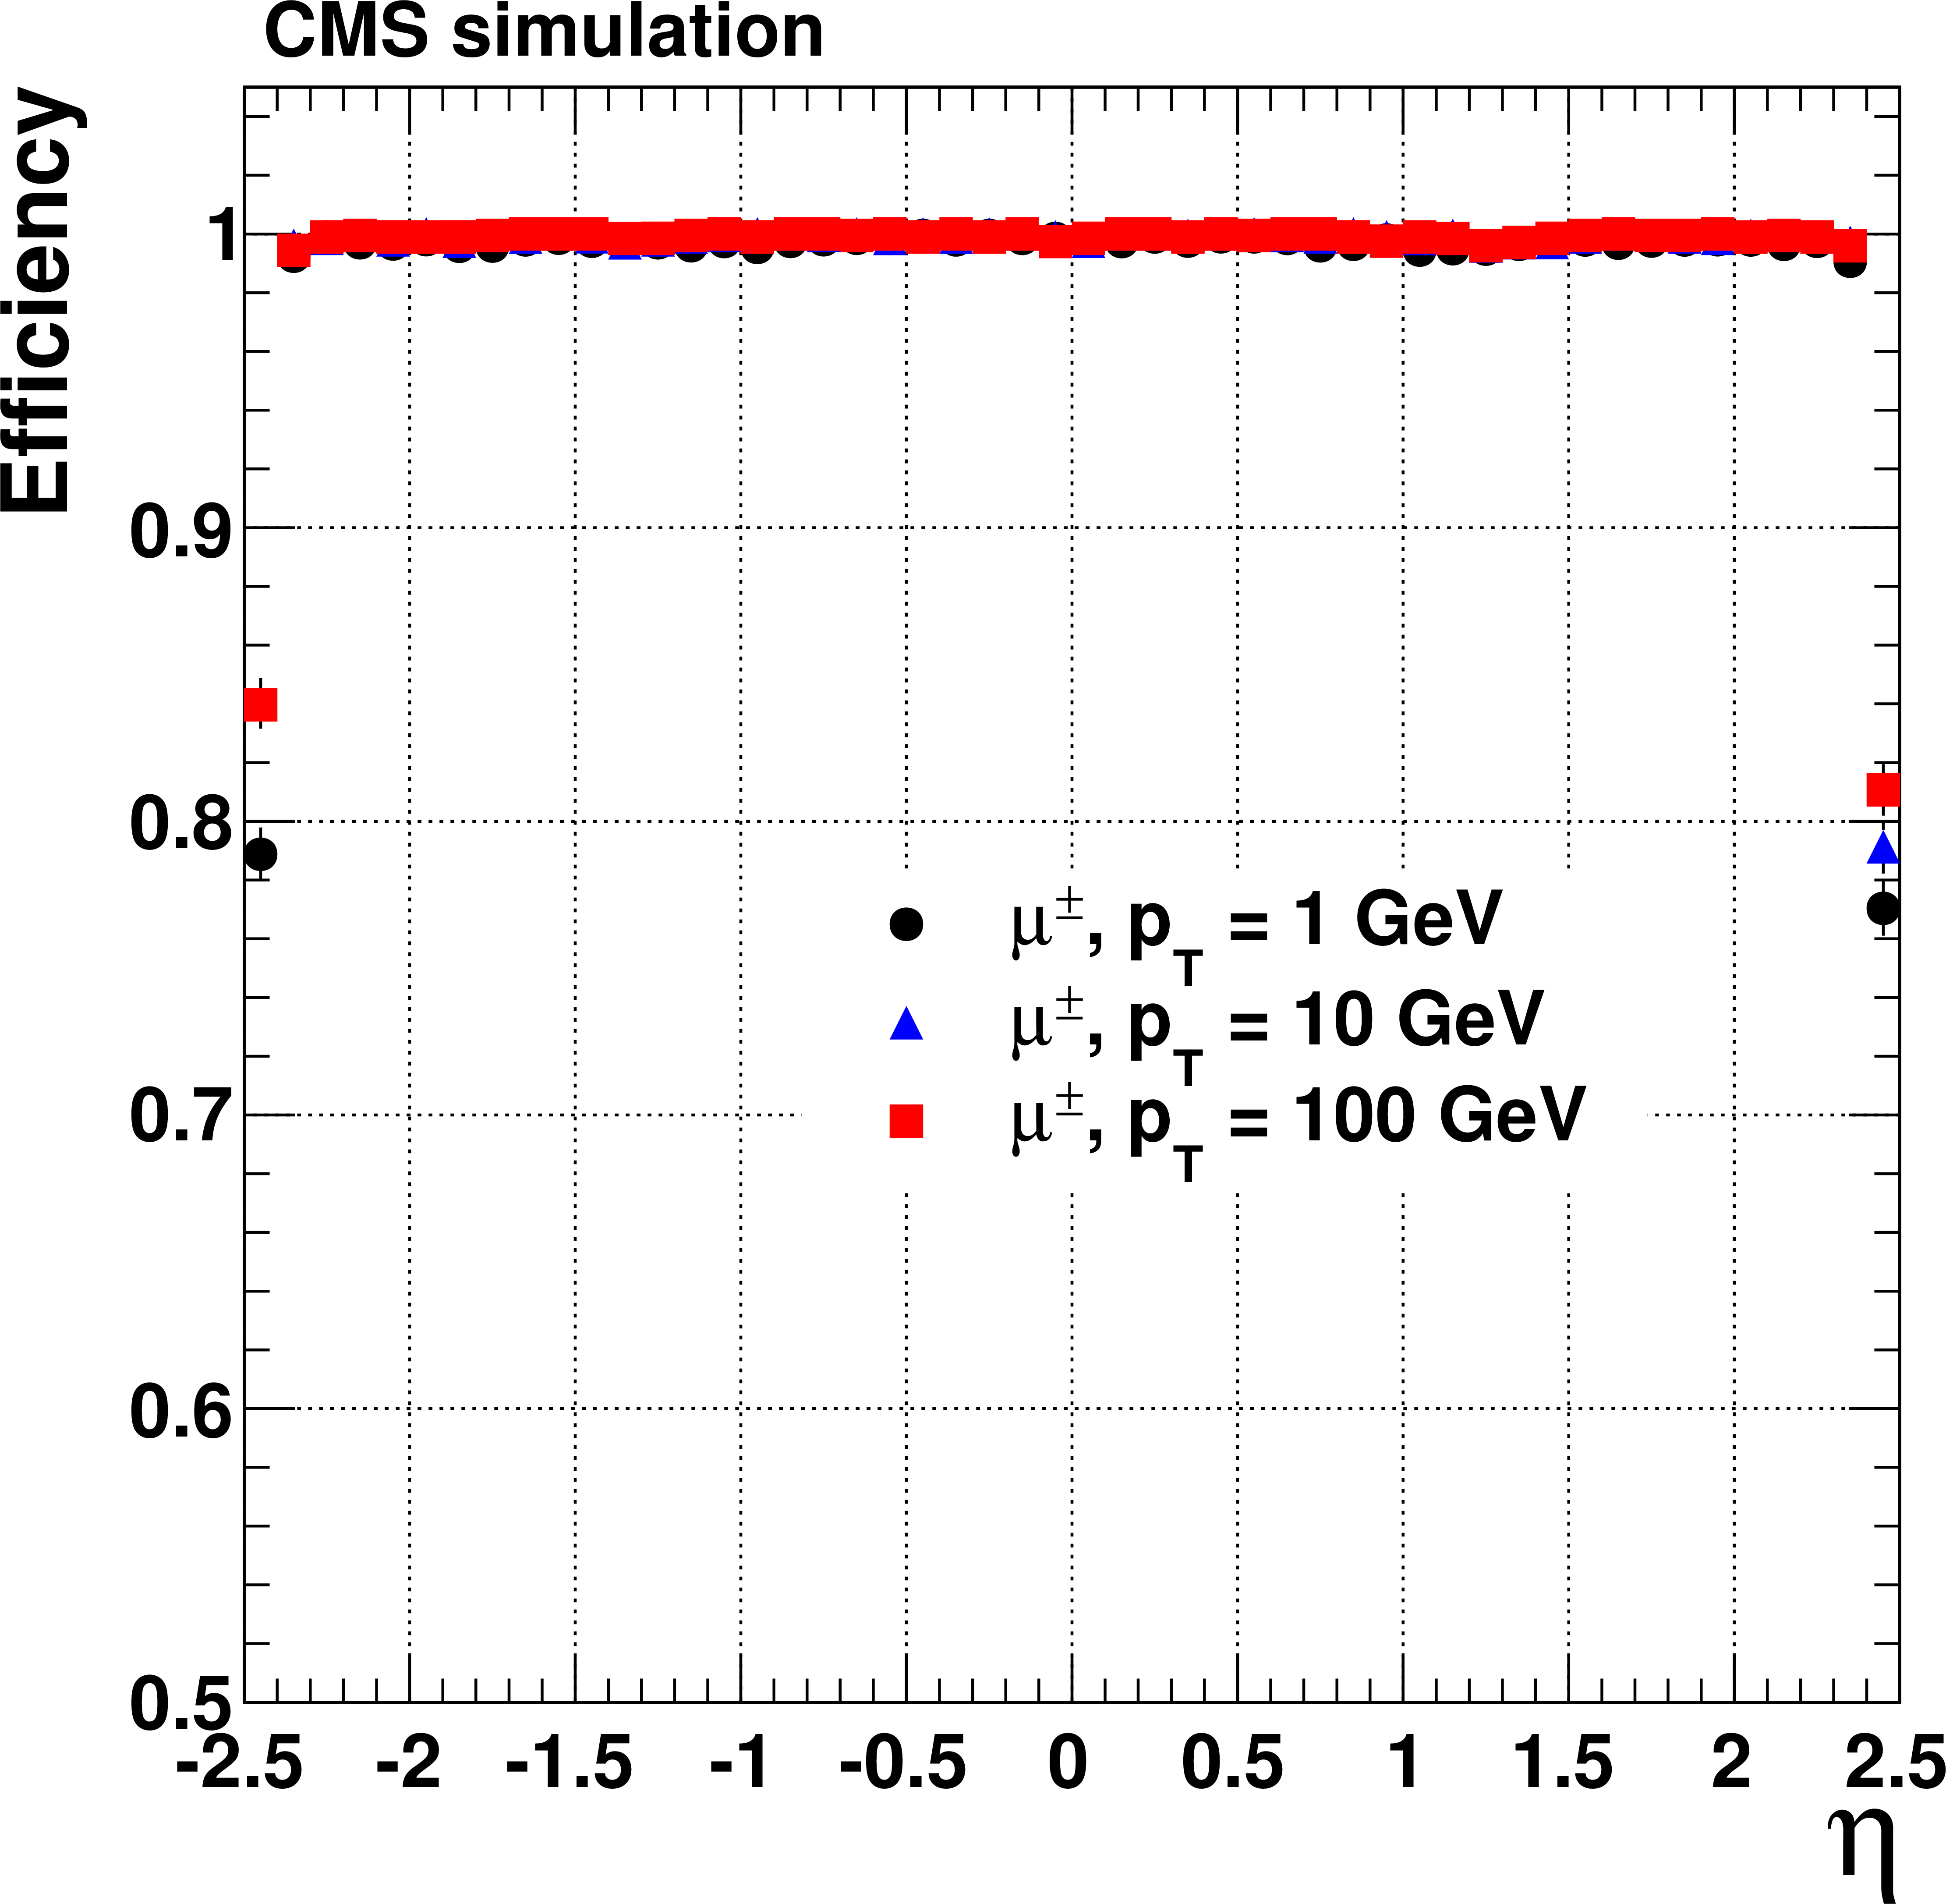
\includegraphics[width=0.45\textwidth]{figs/eff_muon_vs_eta.png}
    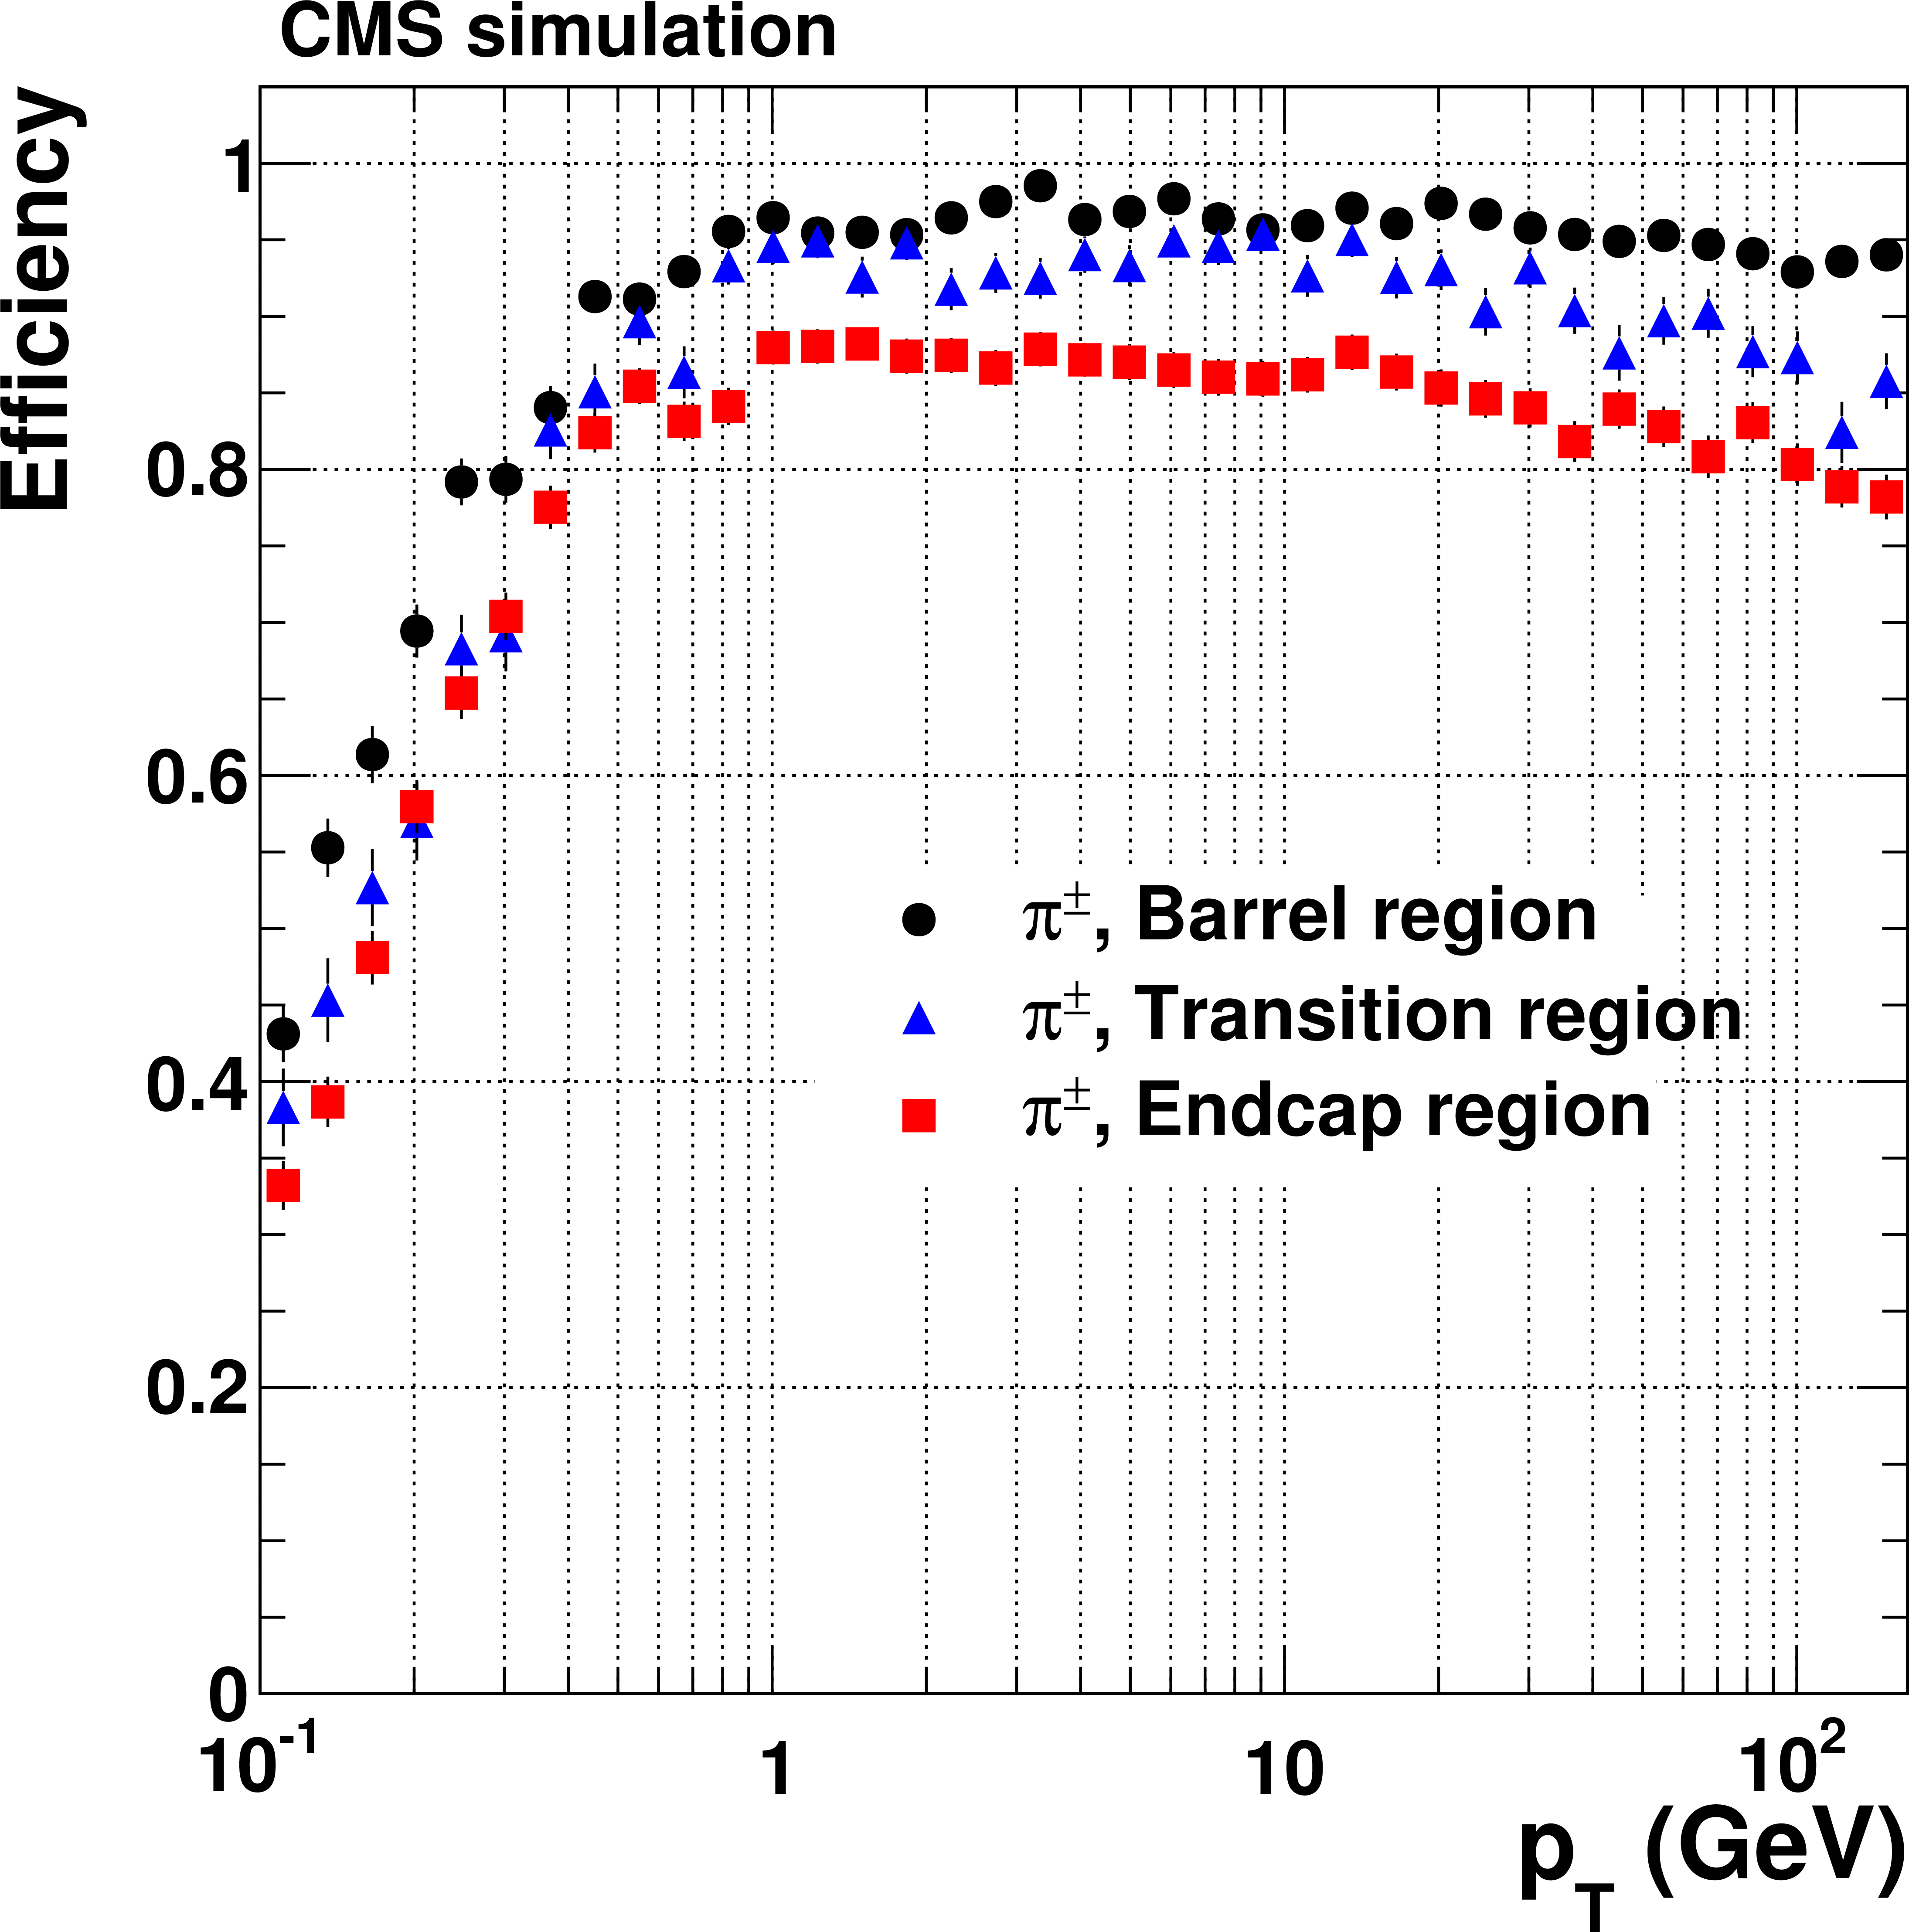
\includegraphics[width=0.45\textwidth]{figs/eff_pion_vs_pt.png}
    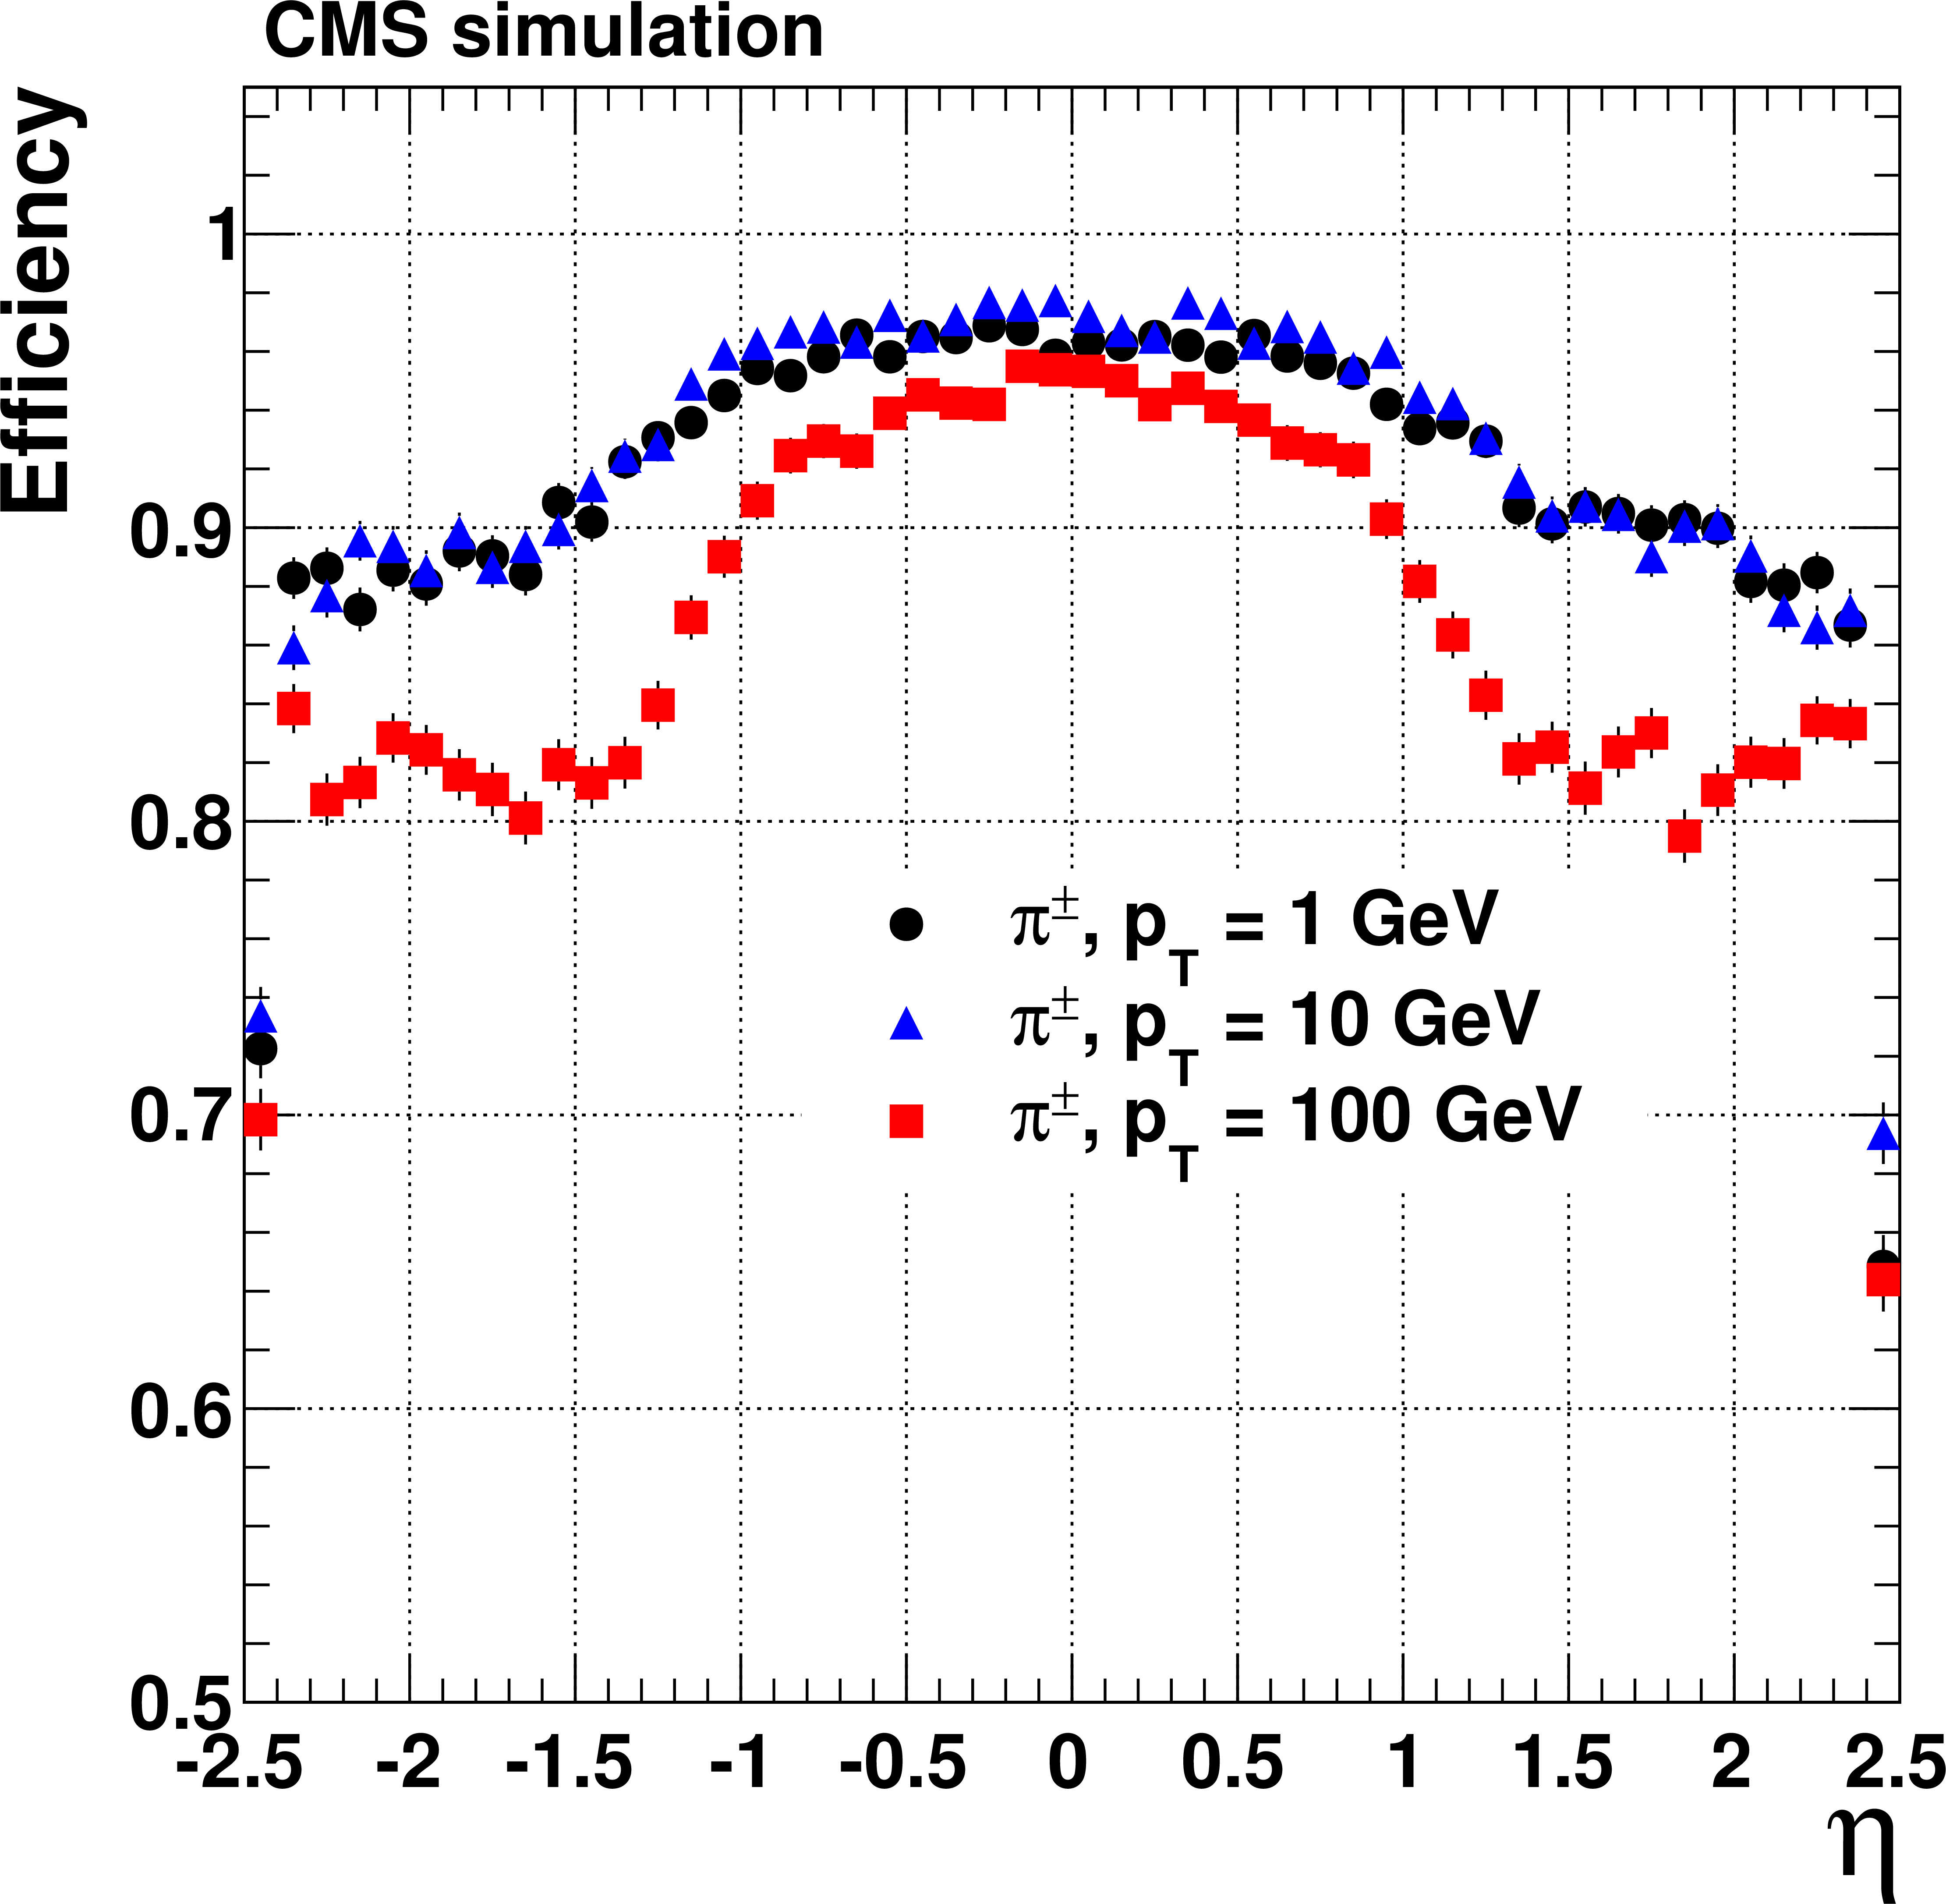
\includegraphics[width=0.45\textwidth]{figs/eff_pion_vs_eta.png}
    \caption{Reconstruction efficiency of charged pions and muons in the tracker system as function of $p_{T}$ and $\eta$. Pions and muons are reconstructed with an efficiency close to one for a $p_{T}>$1 GeV. }
    \label{fig:TrackerEff}
  \end{center}
\end{figure}
%\begin{TOINCLUDE}Plots: Tracker efficiency reconstruction for muons and single pions as function of pt and eta\end{TOINCLUDE}

\subsubsection{Vertex reconstruction}

The problem of vertex finding relies on the association of a set of tracks up to the beam line. A figure of merit is used in order to measure the compatibility of a set of tracks pointing to a given vertex. For such figure of merit, the $z$ position of the tracks, from trajectory extrapolation, and the vertex position are used. The final assigning of vertices respond to the minimization of the figure of merit. Finally, the primary vertex associated to a set of tracks is defined as the one that minimizes the sum of the $p_{T}$ squared, $\sum_{tracks}p_{T}^{2}$, of the associated tracks. The resolution, in $x$ and $z$, and efficiency of primary vertices is presented in figure~\ref{fig:VertexRec}, taken from~\cite{Chatrchyan:2014fea}.

\begin{figure}[!Hhtbp]
  \begin{center}
    %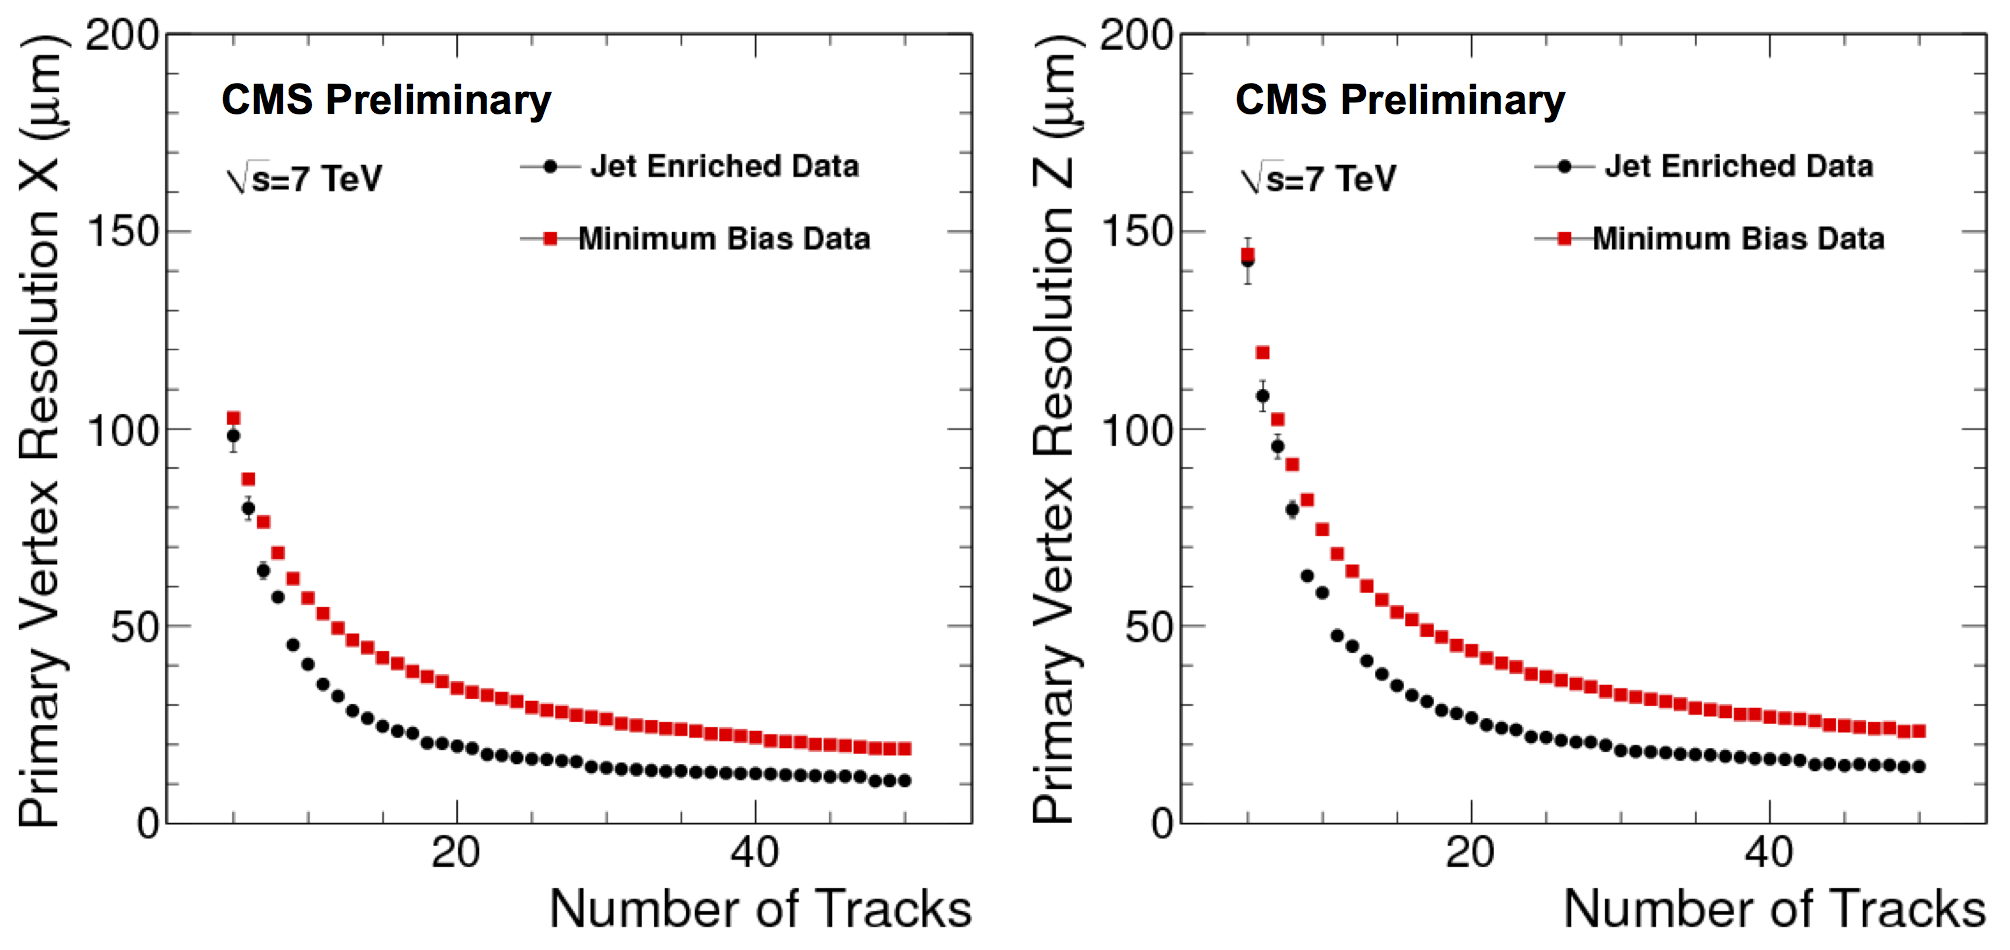
\includegraphics[scale=0.255]{figs/PrimaryVertexResolutions.png}
    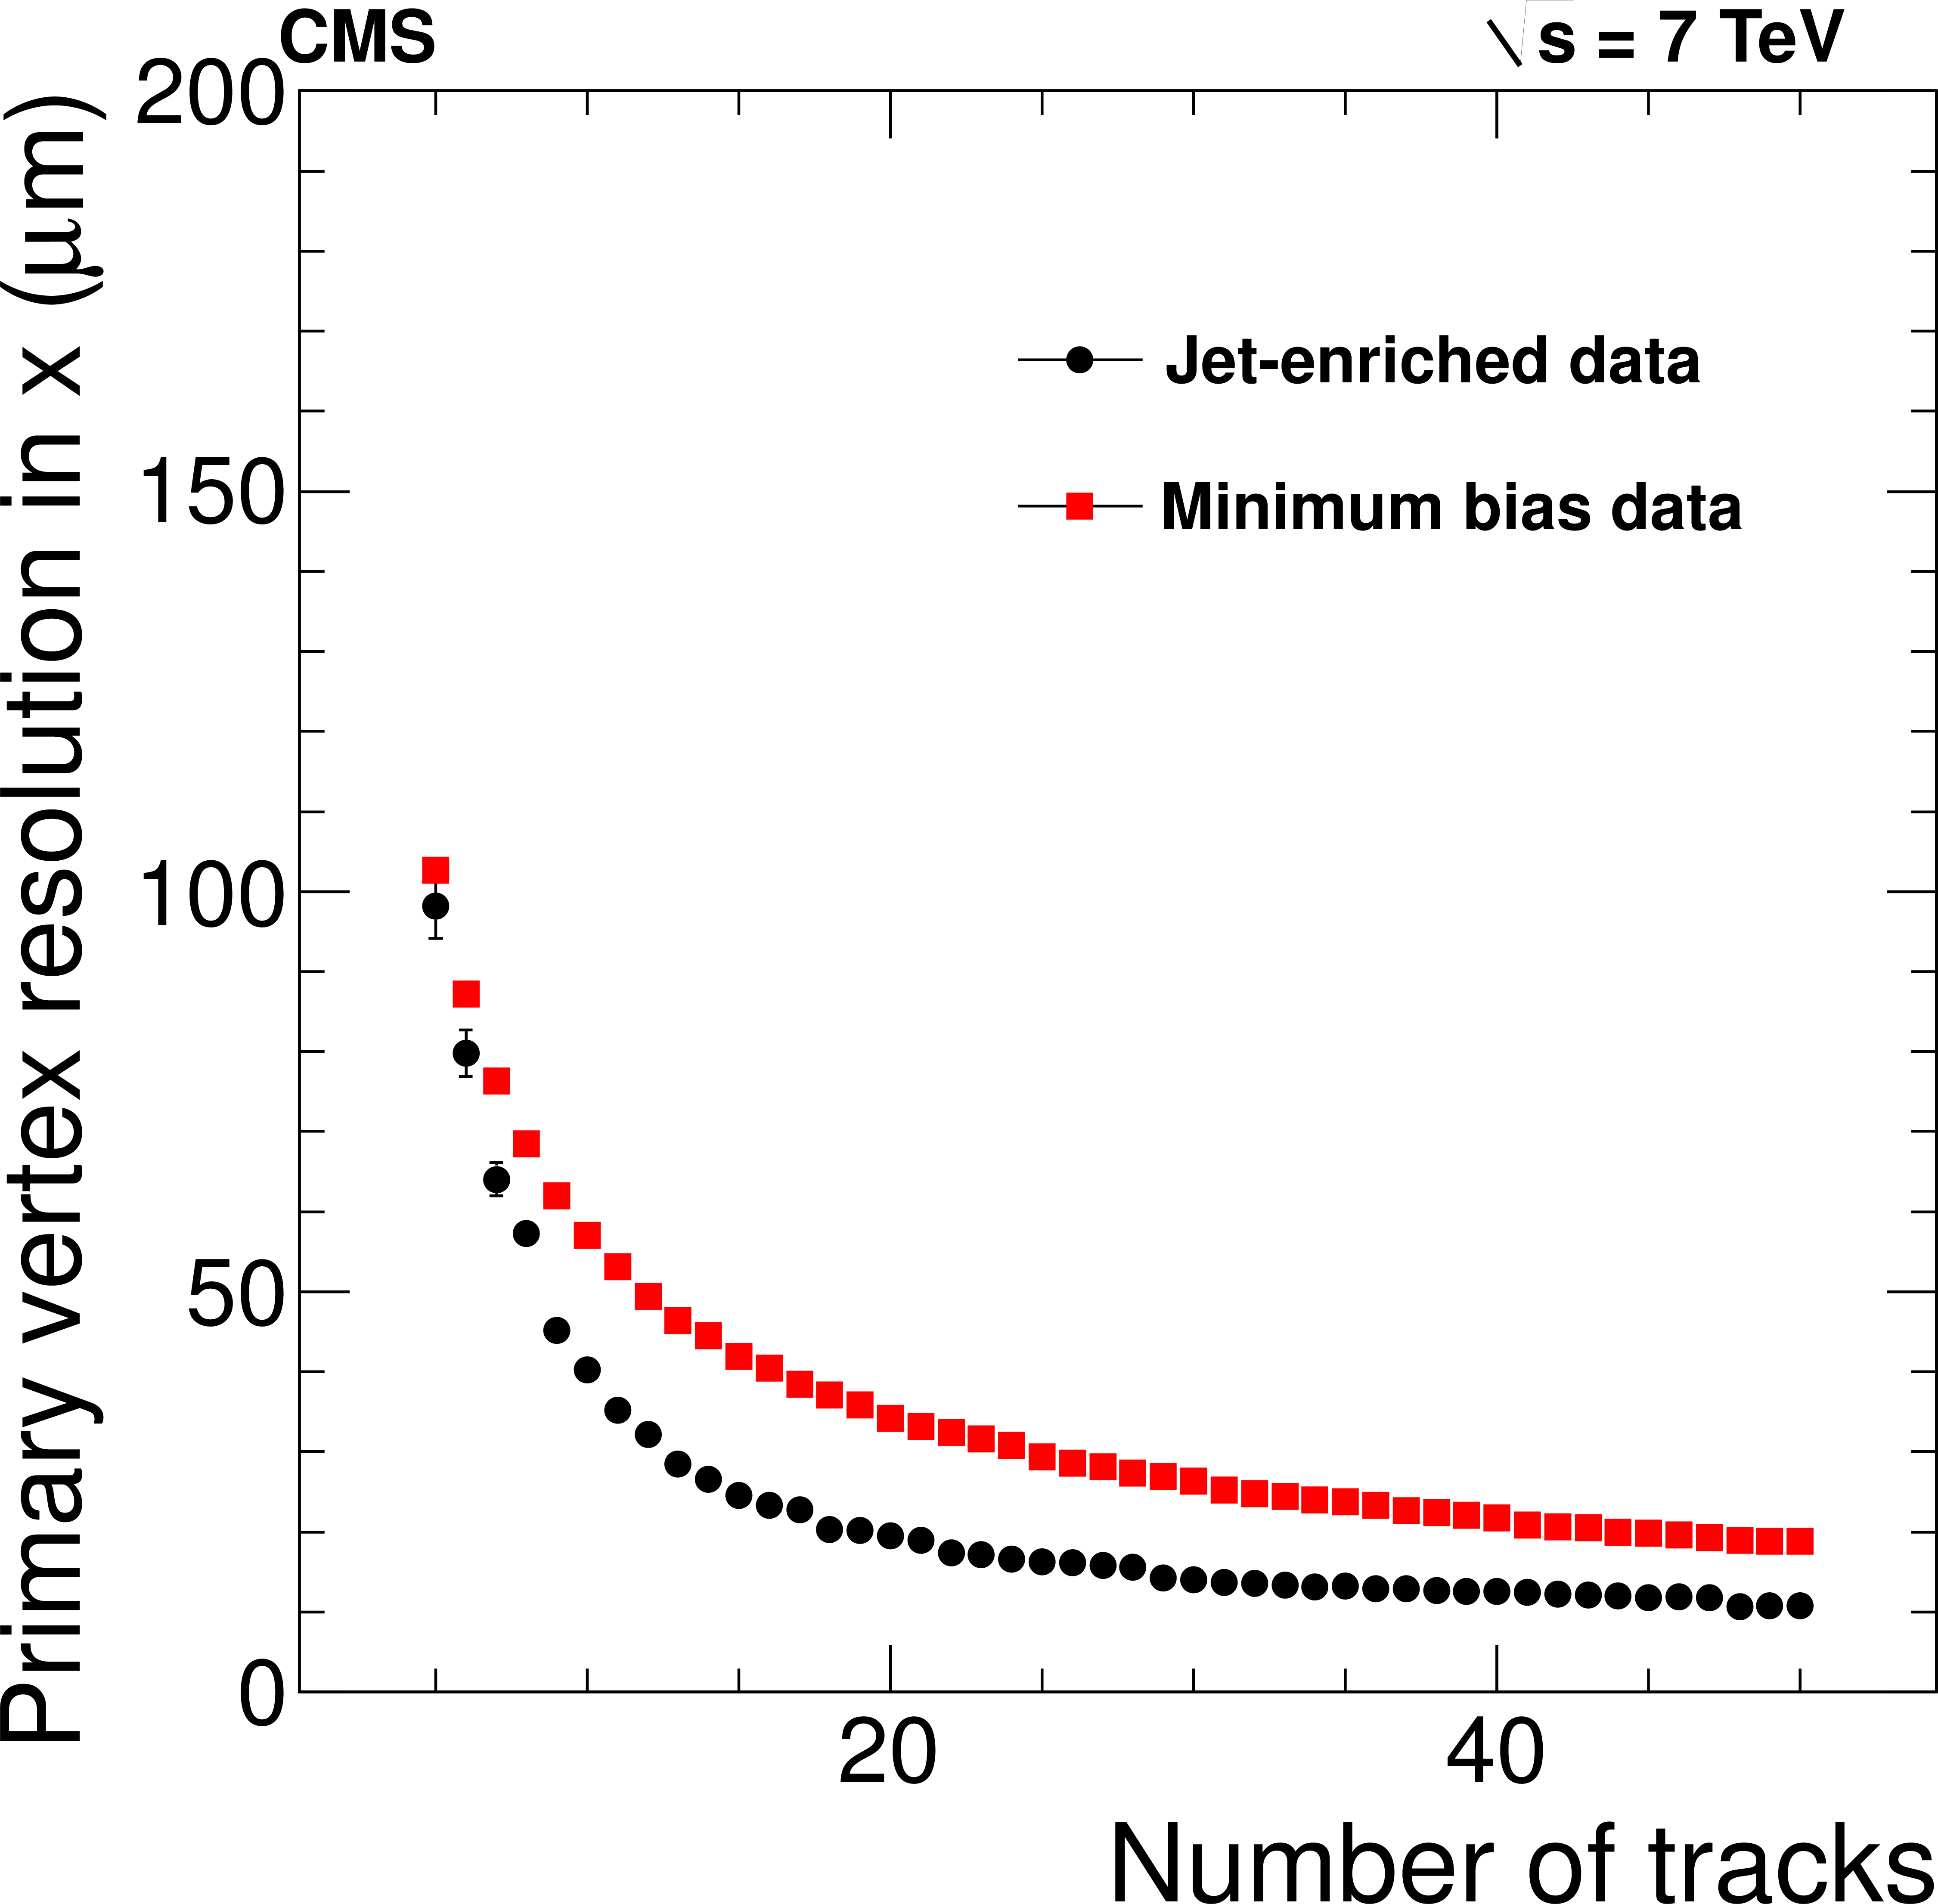
\includegraphics[width=0.3\textwidth]{figs/PrimaryVertexResolutionX.png}
    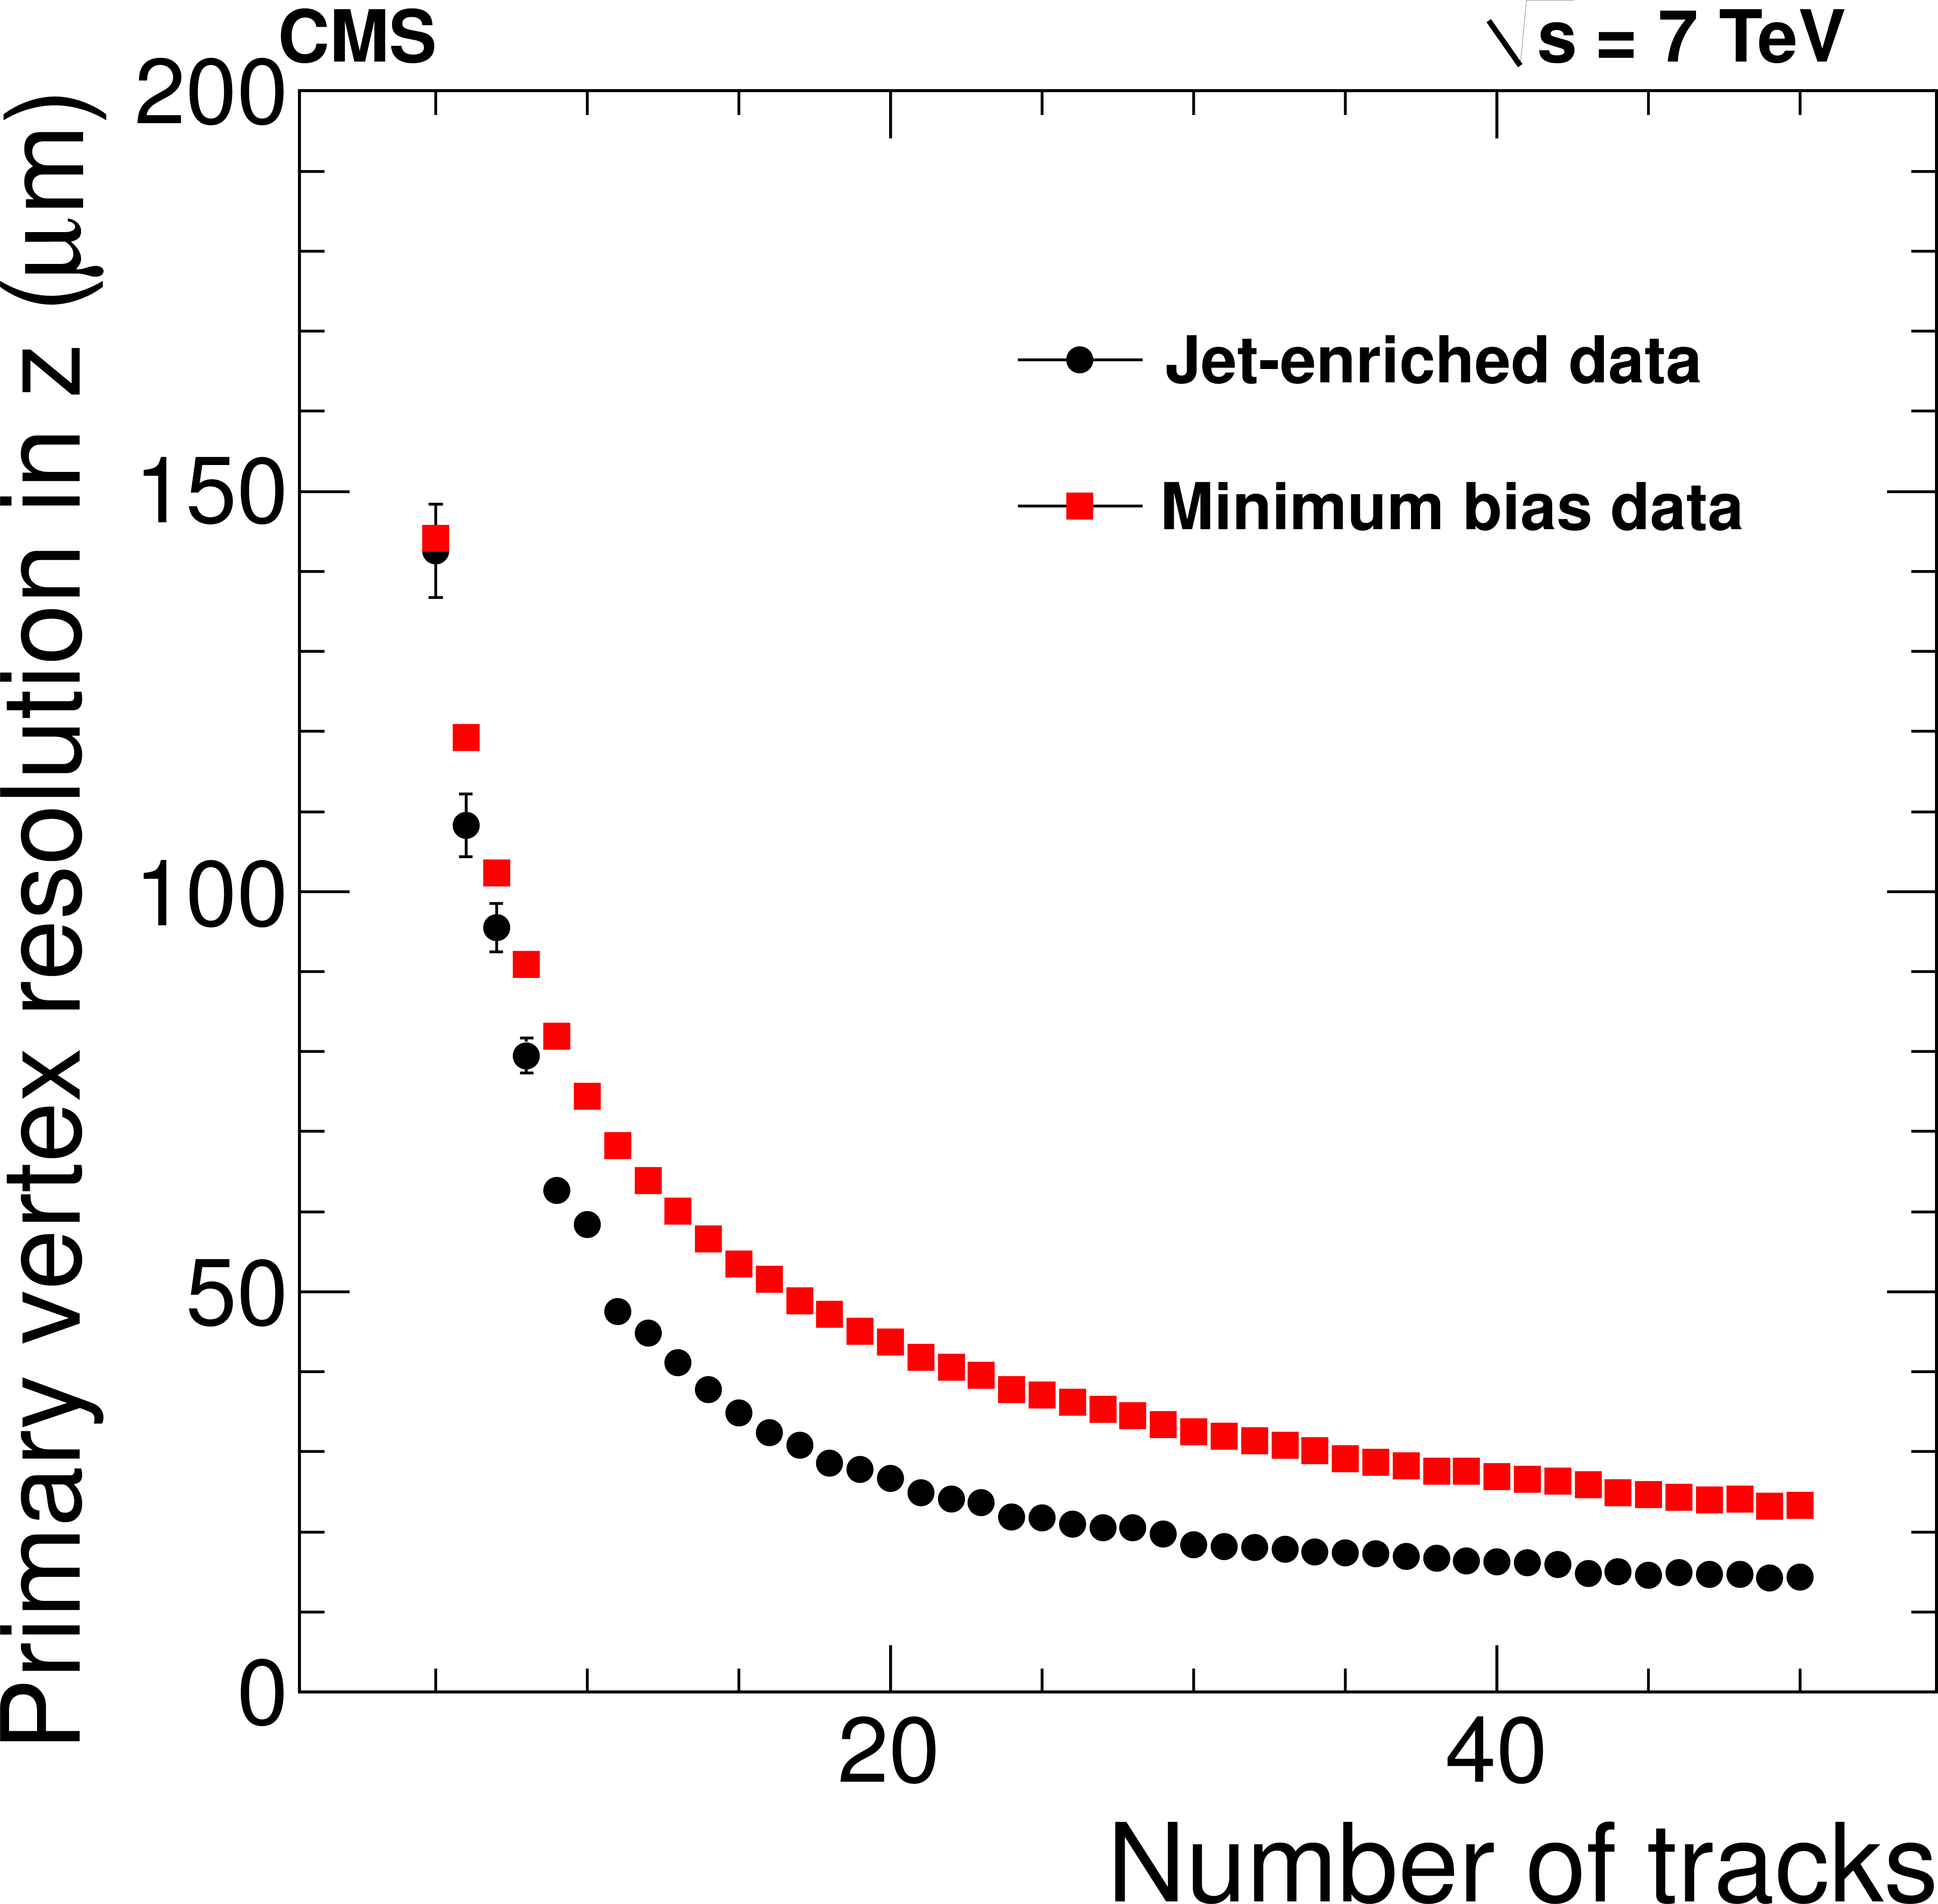
\includegraphics[width=0.3\textwidth]{figs/PrimaryVertexResolutionZ.png}
    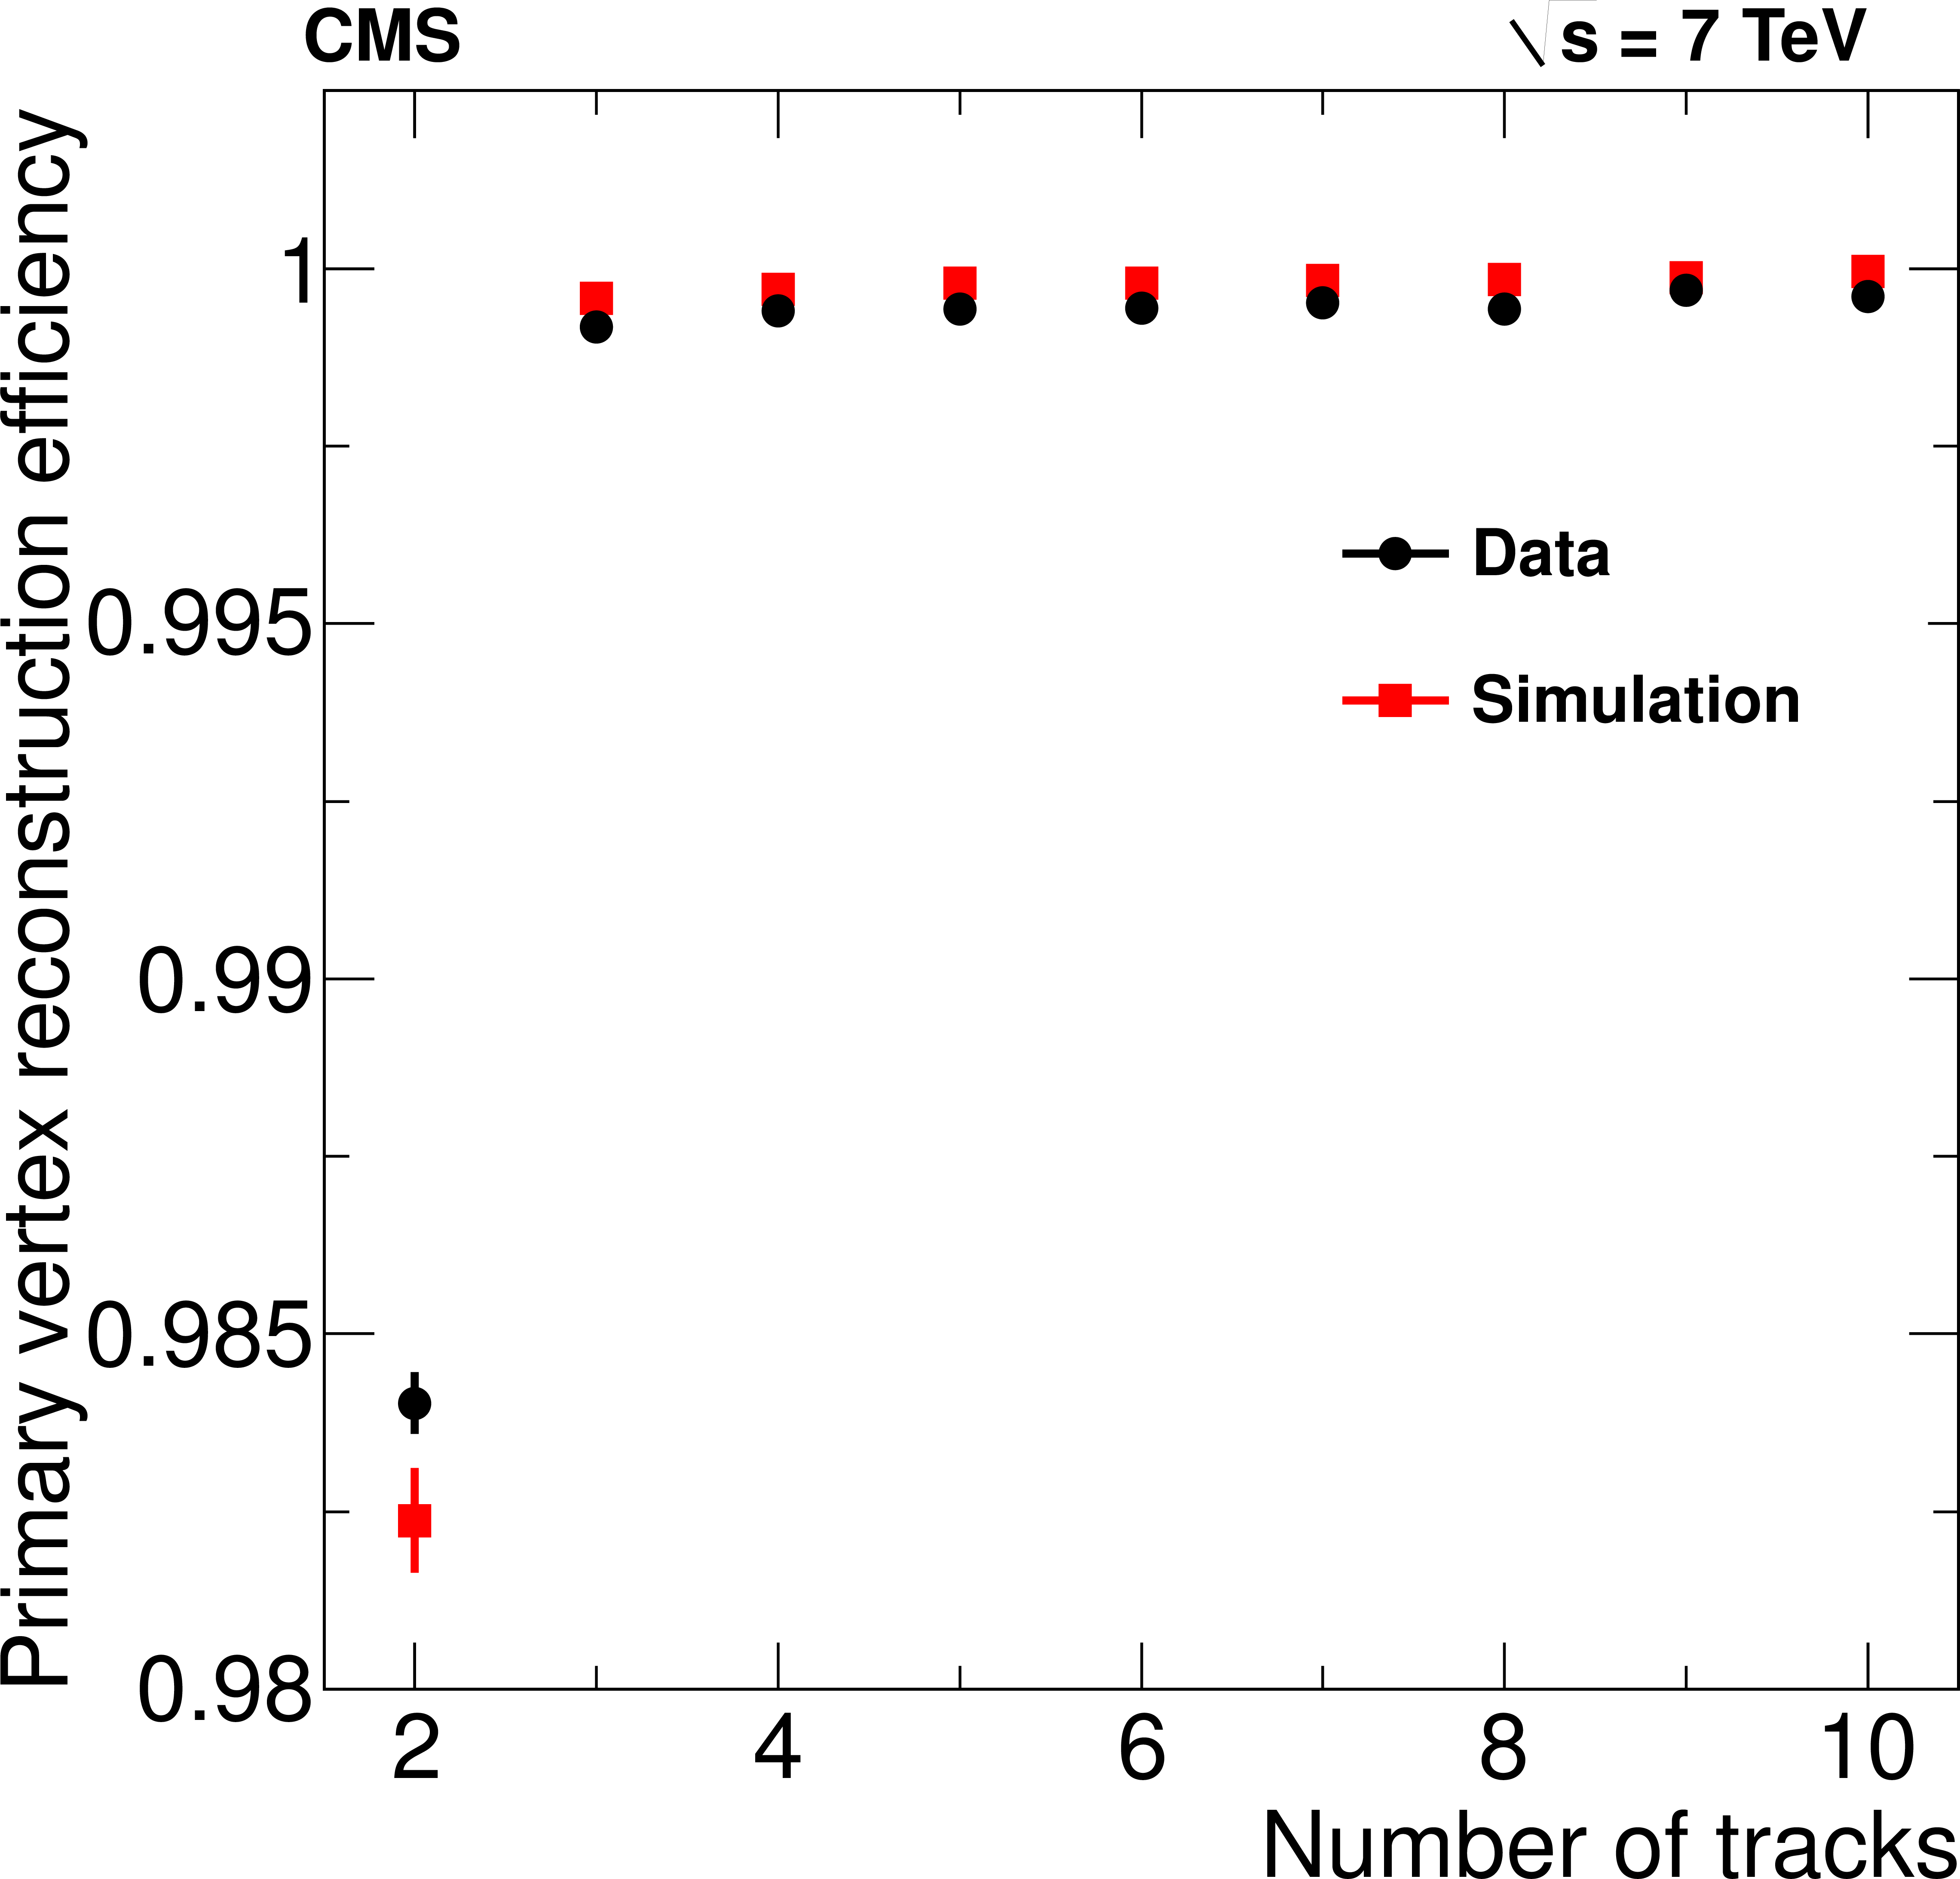
\includegraphics[width=0.3\textwidth]{figs/PrimaryVertexTagAndProbeEfficiency.png}
    \caption{Resolution [left, center] and efficiency [right] of reconstruction of primary vertices. Small differences are seen in the primary vertex reconstruction efficiency between data and Monte-Carlo simulation for events with only 2 tracks.}
    \label{fig:VertexRec}
  \end{center}
\end{figure}
%\begin{TOINCLUDE}Two plots: Primary vertex resolutions and Primary vertex efficiency\end{TOINCLUDE}

\subsubsection{Calorimeter clustering}

Identification of calorimeter cluster is an important step in the reconstruction of particles in CMS. They are defined as a group of deposits in an specific part of a calorimeter. Their reconstruction proceeds from the cell energy maxima, then adjacent deposits are associated to it up to an energy threshold determined to avoid adding noise. The clusters are used in the particle flow algorithm to reconstruct objects, as jets. The procedure is done both in the ECAL and HCAL. Calorimeter clusters are used to identify, for example, neutral hadrons and reconstruct the energy of charged hadrons not correctly reconstructed in the tracker.    

\subsubsection{Subdetectors link}

A single particle traversing CMS may interact with several subdetectors. For example, a charged pion would leave a track, a cluster in the ECAL and a cluster in the HCAL. Then, taking into account the information of different subdetectors and connecting them help to correctly identify each type of particle. Thanks to the excellent granularity of CMS, which allows to have a highly performing linking between different subdetectors, efficient reconstruction algorithms are available. 

The links are done from an extrapolation of tracks towards the calorimeters. A track and a cluster are linked if the extrapolation point is within the cluster boundaries. The extrapolation to the ECAL is performed up to a depth corresponding to the expected maximum of an electromagnetic shower. On the other hand, the extrapolation to the HCAL is performed up to a  depth of a nuclear interaction, characterizing an hadronic shower. Figure~\ref{fig:SubdetConec} shows the links from two tracks linking ECAL and HCAL clusters in $\eta-\phi$ plane, taken from~\cite{Brochet:1956723}. An additional link can also be created between ECAL and HCAL clusters if the position of the electromagnetic cluster is contained in the zone of the hadronic cluster.

\begin{figure}[!Hhtbp]
  \begin{center}
    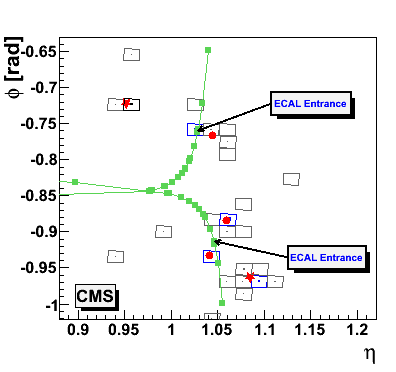
\includegraphics[width=0.4\textwidth]{figs/Conection_tracks_Ecalcluster.png}
    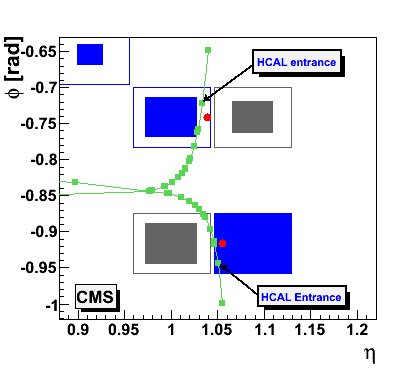
\includegraphics[width=0.4\textwidth]{figs/Conection_tracks_Hcalcluster.png}
    \caption{Connection between tracks reconstructed in the tracker (in green) and energy clusters in the ECAL [left] and HCAL clusters [right].}
    \label{fig:SubdetConec}
  \end{center}
\end{figure}
%\begin{TOINCLUDE}Two plots: Link of tracks to ECAL and to HCAL\end{TOINCLUDE}
%
%\subsubsection{Particle reconstruction}
%
%\subsection{Electron reconstruction}
%Description of variables used to reconstruct electrons.
%\begin{figure}[!Hhtbp]
%  \begin{center}
%    
\includegraphics[width=0.3\textwidth]{figs/CMSlogo.png}
%    \caption{Reconstruction efficiency of electrons.}
%    \label{fig:EleEff}
%  \end{center}
%\end{figure}
%\begin{table}[htbH]
%\label{tab:ElectronParam}
%\begin{center}
%\begin{tabular}{|c|c|c|}
%\hline 
%xxxxxxx & xxxxxxx & xxxxxxx
%\hline
%\end{tabular}
%\caption{Identification requirements for electrons}
%\end{center}
%\end{table}
%\begin{TOINCLUDE}Plot of electron efficiency. Table with electron ID requirements\end{TOINCLUDE}
%
%\subsection{Muon reconstruction}
%
%Muon reconstruction description and goodness of reconstruction from dimuon mass spectra showing resonances.
%
%\begin{figure}[!Hhtbp]
%  \begin{center}
%    
\includegraphics[width=0.3\textwidth]{figs/CMSlogo.png}
%    \caption{Reconstruction efficiency of muons.}
%    \label{fig:MuEff}
%  \end{center}
%\end{figure}
%
%\begin{figure}[!Hhtbp]
%  \begin{center}
%    
\includegraphics[width=0.3\textwidth]{figs/CMSlogo.png}
%    \caption{Dimuon mass spectra from reconstructed muons in CMS.}
%    \label{fig:DiMuonMass}
%  \end{center}
%\end{figure}
%\begin{TOINCLUDE}Plots: PF muon efficiency selection, dimuon mass spectra\end{TOINCLUDE}

\subsection{Jet reconstruction}
\label{sec:jets}

Quarks and gluons produced from a collision cannot be observed directly due to the confinement of strong interactions. After their production, they follow an hadronization process (see section~\ref{sec:hadron}), making principally hadrons that are detected in CMS. The set of hadrons produced in the process is called an hadronization cascade. All the particles produced from an initial quark or gluon define a jet. Ideally a jet should contain the energy of the initial parton that undergoes the hadronization processes. Requiring such, jets could be connected to the partons produced in the collision. The analysis presented in chapter~\ref{chap:search} relies in these objects.

\subsubsection{Jet clustering algorithms}

Particle flow algorithm reconstructs individually each particle produced from a collision event. In order to associate all the different particles identified with particle flow additional, additional algorithms are implemented: Clustering algorithms. As clustering algorithms are only interested in hadronic activity, all isolated leptons in an event are removed from the particle content delivered to the clustering process. Within particle physics experiments, different algorithms have been used. ATLAS and CMS mainly use the anti-kt but CMS also uses Cambridge-Aachen algorithm for many analysis. In the following, these algorithms are going to be described with their specific characteristics. Two types of algorithms exist: cone type clustering (SISCone) and sequential clustering (kT, Cambridge-Aachen, anti-kT). The first type uses a fixed radius circle to try to identify clusters of particles. The second type clusters particles relating them by a distance until a fixed maximal raidus. 

\begin{figure}[!Hhtbp]
  \begin{center}
    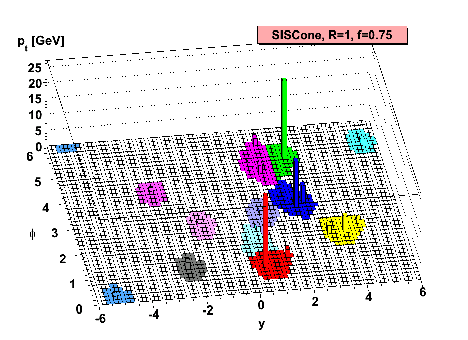
\includegraphics[width=0.43\textwidth]{figs/herwig-parton-level-ev-siscone-R1-0-f0-75-ghosted4root.png}
    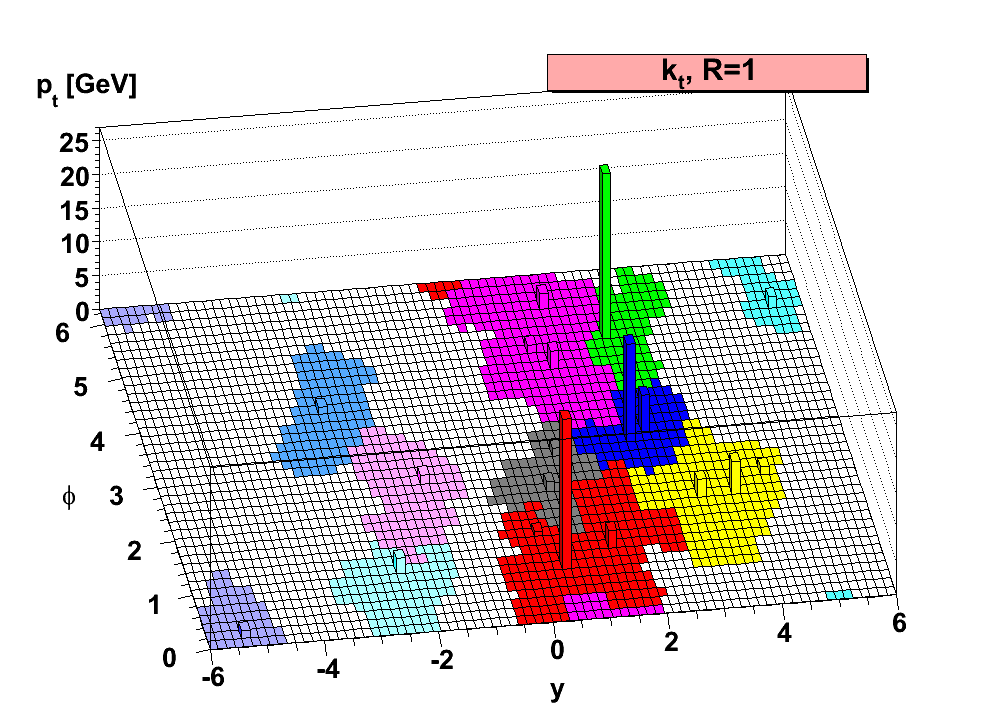
\includegraphics[width=0.43\textwidth]{figs/herwig-parton-level-ev-kt-R1-0-ghosted4root.png}
    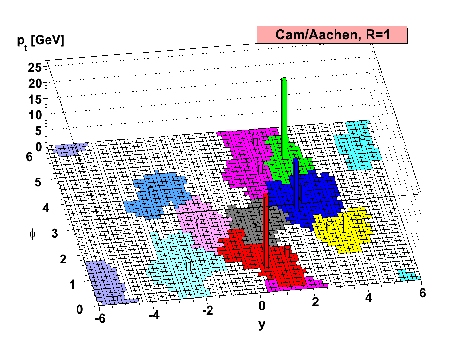
\includegraphics[width=0.43\textwidth]{figs/herwig-parton-level-ev-cam-R1-0-ghosted4root.png}
    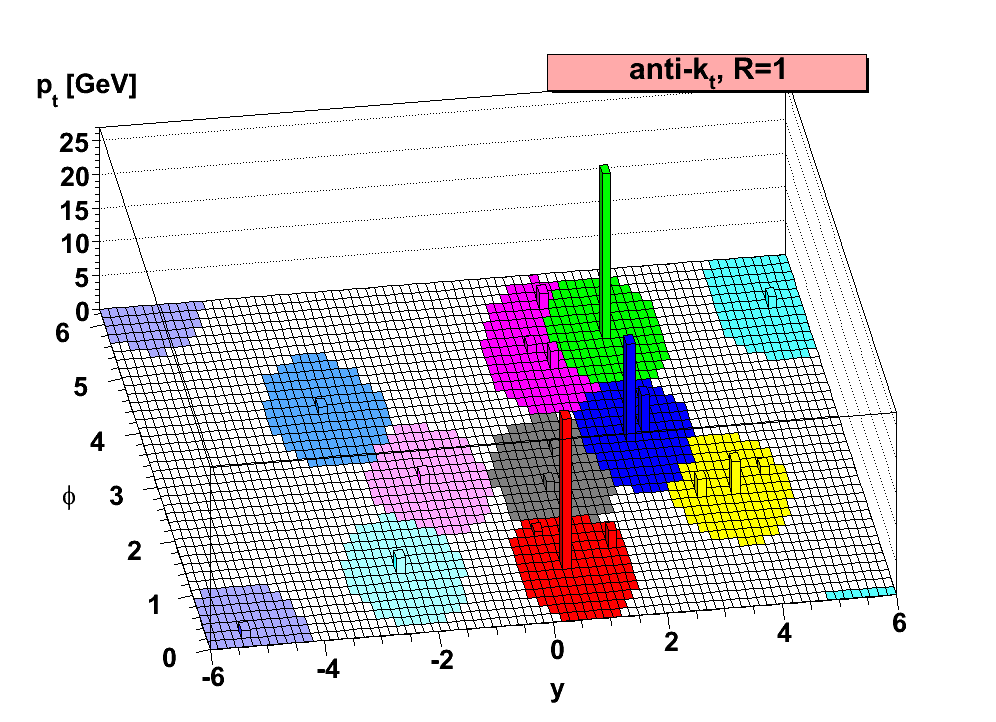
\includegraphics[width=0.43\textwidth]{figs/herwig-parton-level-ev-antikt-R1-0-ghosted4root.png}
    \caption{Jets in a Monte-Carlo event reconstructed with four different clustering algorithms: SISCone [left-up], kT [right-up], Cambridge-Aachen [left-down] and anti-kT [right-down]. All algorithms used same radius $R=1$. Jets displayed in the $y-\phi$ plane and reconstructed $p_{T}$ in the z-axis. From~\cite{Cacciari:2008gp}.}
    \label{fig:JetsAlgos}
  \end{center}
\end{figure}

\paragraph{SISCone}

SISCone algorithm~\cite{Salam:2007xv} uses a circle to explore randomly the $\eta-\phi$ plane until a particle comes into contact with it. Then the circular enclosure is pivoted until a second particle touches the edge. All the matches define the stable cones. Particles in the found stable cones are removed and the procedure is repeated until no more cones are found. From all found stable cones an algorithm is used to split or merge the cones in final jets based on an overlap parameter. In figure~\ref{fig:JetsAlgos} an example of the jets reconstructed by SISCone can be seen for a circular enclosure of radius 1. 

\paragraph{kT}

kT-algorithm~\cite{Ellis:1993tq} is one of the most used jet reconstruction algorithms. It begins with the calculation of the kT distance for all pair of particles ($i$,$j$), defined as

\begin{equation}
  \label{eq:kt}
  d_{ij}=min(p_{Ti}^{2},p_{Tj}^{2})\Delta R_{ij}^{2}/R^{2}
\end{equation} where $\Delta R_{ij}^{2}=(y_{i}-y_{j})^{2}+(\phi_{i}-\phi_{j})^{2}$ and $R$ is the radius parameter. The distance of a particle to the beam is $d_{iB}=p_{Ti}^{2}$. 

Then the minimal distance between all $d_{ij}$ and $d_{iB}$ is found, if it is a $d_{ij}$ the two particles are merged, if it is a $d_{iB}$ the particle is declared to be a final jet. The process is repeated until no particles are left. A result of this reconstruction can be found in figure~\ref{fig:JetsAlgos}. 

\paragraph{Cambridge-Aachen}

Cambridge-Aachen (CA) jet algorithm is similar to kT algorithm but changes the distance definition to $d_{ij}=\Delta R_{ij}^{2}/R^{2}$ and $d_{iB}=1$. In figure~\ref{fig:JetsAlgos} it can be seen the jets produced by this algorithm.

\paragraph{Anti-kT}

Anti-kT (AK) algorithm proceeds equivalently to kT and CA algorithms changing the definition of distance to

\begin{equation}
  \label{eq:antikt}
  d_{ij}=min\left(\frac{1}{p_{Ti}^{2}},\frac{1}{p_{Tj}^{2}}\right)\Delta R_{ij}^{2}/R^{2};\; d_{iB}=\frac{1}{p_{Ti}^{2}}
\end{equation} 

This algorithm produces ``perfectly'' circular conic jets. An example of the reconstruction performed by this algorithm can be seen in figure~\ref{fig:JetsAlgos}.

\paragraph{Infrared and collinear safety}

Two extremely important characteristics that should be achieved correctly by jet algorithms are to be collinear and infrared safe. In QCD processes, a parton can split in two collinear components or can emit soft radiation. Such processes will give rise to extra hadrons that could lead to ambiguities in the jet reconstruction, giving different jet compositions of an event. Collinear and infrared safety correspond to the ability of an algorithm to give the same results independently if an initial parton radiated or not. In other words, the jet reconstruction should include this radiation correctly to the same jet and do not give rise to an additional jet coming only from one of these radiations. The formerly described jet algorithms are both collinear and infrared safe, well reconstructing jets to solely initial partons. 

\paragraph{Jet area}

Jet area, discussed in~\cite{Cacciari:2008gn}, is a concept used to estimate the sensitivity of jet algorithms to radiation or pileup or underlying event. Naively, the area of the jet is expected to correspond to $\pi R^{2}$, where $R$ is the radius parameter used by the algorithm. Obviously, this parameter is also related to the final shape of jets given by the algorithm. From figure~\ref{fig:JetsAlgos} one can see in the $y-\phi$ plane the area given by SISCone, kT, CA and AK algorithms. Closer the area to the expected value less sensitive is the algorithm to radiation, making it more stable to real experimental conditions, where pileup and underlying event contributions could be high. A more precise way to estimate the stability of an algorithm, in terms of area, is to measure the jet area and compare it to the expected area scanning it as function of the jet $p_{T}$. In figure~\ref{fig:JetsAlgosArea} can be seen such study, from it one can see that AK algorithm is the most stable one. This behavior constitutes a powerful reason to prefer AK over other algorithms. 

\begin{figure}[!Hhtbp]
  \begin{center}
    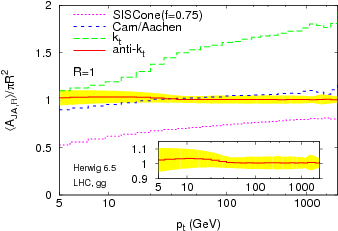
\includegraphics[width=0.45\textwidth]{figs/JetArea.png}
    \caption{Jet areas over expected geometrical jet area for different jet algorithms as function of the reconstructed $p_{T}$. From~\cite{Cacciari:2008gp}.}
    \label{fig:JetsAlgosArea}
  \end{center}
\end{figure}
%\begin{TOINCLUDE}Plots: Jet in y-phi-pT space for each algorithm\end{TOINCLUDE}

\paragraph{Reconstruction at CMS}

CMS experiment uses AK algorithm with a radius of 0.5 to reconstruct jets. Alternatively CA with radius of 0.8, 1.0 or 1.5 are also used to identify jets substructure, jets inside jets. AK reconstruction relies on particles reconstructed by the particle flow algorithm, being then called particle flow jets (PFJets). In figure~\ref{fig:PFJets} it can be seen the composition of PFJets.  

 \begin{figure}[!Hhtbp]
  \begin{center}
    \includegraphics[width=0.4\textwidth]{figs/Jet_composition_data_7TeV.png}
    \begin{minipage}[t]{.15\textwidth}
      \centering
      \includegraphics[width=1.0\textwidth]{figs/Legend_jet_composition.png}
    \end{minipage}
    \includegraphics[width=0.4\textwidth]{figs/Jet_composition_MC_7TeV.png}
    \caption{Jet composition fraction of particle flow jets as function of $\eta$ for data [left] and Monte-Carlo simulation [right]. From~\cite{Beaudette:2014cea}. Central jets $|\eta|<2.5$ are composed $\sim$ 60\% by charged hadrons and the rest by neutral particles (hadrons and photons) }
    \label{fig:PFJets}
  \end{center}
\end{figure}

\subsubsection{Jet energy corrections}

Whereas jet reconstruction algorithms have been tuned to give the best performance possible, in real experiments the reconstruction is not perfect. Some times all the information in the detector, tracks or calorimeter clusters, are not available or just partially. This impacts jet properties, as for example the $p_{T}$. Data-driven methods, as in~\cite{2011JInst...611002C}, have been implemented in CMS to correct such imperfections and to measure the resolution of the reconstructed jets in $p_{T}$. Several correction levels have been considered in order to take into account subdetectors response to pileup, particle content in different eta regions, among others. In general, such corrections are called Jet Energy Corrections (JEC). 

The most important information to determine from jet reconstruction are the energy scale and resolution, correspondingly called Jet Energy Scale (JES) and Jet Energy Resolution (JER). Uncertainties in these quantities depend on the reconstructed $p_{T}$ of the jets and on $\eta$, they can be seen in figure~\ref{fig:JEC}. JEC uncertainties are of the order of 1\% for central jets with $p_{T}>100$ GeV/c.

\begin{figure}[!Hhtbp]
  \begin{center}
    \includegraphics[width=0.4\textwidth]{figs/JEC_pt.png}
    \includegraphics[width=0.4\textwidth]{figs/JEC_eta.png}
    \caption{JEC uncertainties as function of $p_{T}$ [left] and $\eta$ [right]. From~\cite{Brochet:1956723}. JEC have an uncertainty smaller than 4\% for jets with $p_{T}>$ 20 GeV, what shows the reliability of jet reconstruction.}
    \label{fig:JEC}
  \end{center}
\end{figure}
%\begin{TOINCLUDE}Plot of JEC uncertainity as pT function and eta\end{TOINCLUDE}

\subsubsection{b-jets identification}
\label{sec:bid}

B-quarks produced in a collision hadronize forming B-hadrons. These hadrons differentiate from the rest due to their stability, taking more time to decay in average than unstable hadrons with only $u$ or $d$ quarks. This additional time of flight is seen in the detector as a displaced vertex. This characteristic is one of the principal handles to identify jets coming from an initial b-quark. Complex algorithms have been developed in CMS to study and combine jet information to attribute a probability of coming from a b-quark to each jet.  

\paragraph{Identification algorithms and working points}

CMS collaboration uses for b jet identification, called b-tagging, the Constrained Secondary Vertex (CSV) algorithm~\cite{Chatrchyan:2012jua, CMS:2013vea}. The main variable used by the algorithm is the existence of a displaced vertex. Specific parameters of the displaced vertex are used, as the time of flight, its mass, the number of tracks associated to it. The impact parameter is taken into account, because for jets coming from B-hadrons this variable has usually a higher value than for the rest of jets. CSV algorithm takes all this variables and use a MVA (Multivariate Variable Analysis) to build up a discriminant. On the value of the discriminant three cuts are defined. They define the working points that allow to select whether with a high efficiency (loose working point: CSVL) or highly pure sample on b-tags (tight working point: CSVT). The middle working point, CSVM, allows a high efficiency while preserving high purity. In figure~\ref{fig:CSVVar} can be seen the number of secondary vertices and final discriminator for CSV algorithm.

\begin{figure}[!Hhtbp]
  \begin{center}
    \includegraphics[width=0.4\textwidth]{figs/sv_multi_0_Log.png}
    \includegraphics[width=0.4\textwidth]{figs/pdf-sub.png}
    \caption{Number of secondary vertices [left] and CSV final discriminator [right] for each jet flavor, from QCD Monte-Carlo sample. From~\cite{CMS-PAS-BTV-13-001}.}
    \label{fig:CSVVar}
  \end{center}
\end{figure}

CSVM corresponds to a cut on the discriminator greater than 0.679. This working point has an average efficiency of correctly tagged b-jets of $\epsilon^{CSVM}_{b}\sim$70\%, also the efficiency to tag as b-jet a c-jet is around $\epsilon^{CSVM}_{c}$20\% and any light jet $\epsilon^{CSVM}_{l}\sim$1\%. Two additional working points are defined, a tight working point with the lowest fake rate of b-jets ($\epsilon^{CSVT}_{b}=50$\%, $\epsilon^{CSVT}_{c}=7$\%, $\epsilon^{CSVT}_{l}=0.2$\%) and a loose working points with a higgh b-jet b-tagging efficiency ($\epsilon^{CSVL}_{b}=85$\%, $\epsilon^{CSVL}_{c}=45$\%, $\epsilon^{CSVL}_{l}=10$\%). When the algorithm is applied to Monte-Carlo, a correction has to be performed in order to match the same behavior than in data. Scale factors are derived from the comparison of data and Monte-Carlo. For CSVM a correction of around 5\% to correctly tagged b-jets and to incorrectly b-tagged jets of 17\%. In figure~\ref{fig:CSVEff} can be seen b-tagging efficiencies for CSVM working point as function of jets $p_{T}$ and $\eta$.  

\begin{figure}[!Hhtbp]
  \begin{center}
    \includegraphics[width=0.42\textwidth]{figs/LTdilep_csvMeffeta.png}
    \includegraphics[width=0.42\textwidth]{figs/LTdilep_csvMeffpt.png}
    \caption{Efficiency of CSV b-tagging algorithm in the medium working point as function of jet $p_{T}$ and $\eta$. From~\cite{CMS-PAS-BTV-13-001}.}
    \label{fig:CSVEff}
  \end{center}
\end{figure}
%\begin{TOINCLUDE}Plots: CSV discriminator, Nb of secondary vertices, Efficiency of b-tagging for CSVM as function of PT and eta\end{TOINCLUDE}

%\subsection{Photon reconstruction}
%
%\begin{TOINCLUDE}Plot of photon identification efficiency\end{TOINCLUDE}
%
%\subsection{Missing energy reconstruction}
%
%
%Add RUNII perspectives? Add section on dataset structure used by CMS?
%
%  LocalWords:  emittance ApparatuS
